% !TeX program = xelatex
% !TeX encoding = UTF-8
% =====================================================================
%  รายงานโครงงานคอมพิวเตอร์ CP352101
%  การประยุกต์ใช้การเรียนรู้ของเครื่องเพื่อทำนายฤทธิ์ทางชีวภาพ
%  ของสารยับยั้ง SARS-CoV-2 Main Protease แบบ In Silico
%
%  คอมไพล์ด้วย:  xelatex report.tex   (รัน 2 ครั้งเพื่อให้สารบัญถูกต้อง)
%  หรือ:         latexmk -xelatex report.tex
%  หรือ:         build.bat
% =====================================================================
\documentclass[12pt, a4paper, oneside]{report}

% ---------- การตั้งค่าและแพ็กเกจ (Preamble & Commands) ----------
% ==========================================================
%  preamble/preamble.tex — การตั้งค่าเอกสารและแพ็กเกจหลัก
% ==========================================================

\usepackage{fontspec}
\usepackage{geometry}
\usepackage{graphicx}
\usepackage{booktabs}
\usepackage{longtable}
\usepackage{array}
\usepackage{multirow}
\usepackage{amsmath, amssymb}
\usepackage{caption}
\usepackage{float}
\usepackage{xcolor}
\usepackage{enumitem}
\usepackage{fancyhdr}
\usepackage{titlesec}
\usepackage{tabularx}
\usepackage{ragged2e}
\usepackage[hidelinks, bookmarks=true, bookmarksnumbered=true]{hyperref}

% ---------- ระยะขอบตามมาตรฐานวิทยานิพนธ์ ----------
\geometry{a4paper, top=3.0cm, bottom=2.5cm, left=3.5cm, right=2.5cm}

% ---------- เส้นทางค้นหารูปภาพ (Graphics Path) ----------
\graphicspath{{../figures/}{./figures/}}

% ---------- ฟอนต์ไทย: เลือกอัตโนมัติตามที่มีในเครื่อง ----------
% ลำดับความสำคัญ: TH Sarabun New (มาตรฐานราชการ) > Leelawadee UI > Angsana New > Tahoma
\newcommand{\THAIFONT}{}
\IfFontExistsTF{TH Sarabun New}{
  \renewcommand{\THAIFONT}{TH Sarabun New}
}{
  \IfFontExistsTF{Leelawadee UI}{
    \renewcommand{\THAIFONT}{Leelawadee UI}
  }{
    \IfFontExistsTF{Angsana New}{
      \renewcommand{\THAIFONT}{Angsana New}
    }{
      \renewcommand{\THAIFONT}{Tahoma}
    }
  }
}

% AutoFakeSlant/AutoFakeBold ช่วยให้ฟอนต์ไทยที่ไม่มีตัวเอียงยังแสดงผลได้
\setmainfont{\THAIFONT}[Ligatures=TeX, AutoFakeSlant=0.2, AutoFakeBold=1.5]
\setsansfont{\THAIFONT}[Ligatures=TeX, AutoFakeSlant=0.2, AutoFakeBold=1.5]
\newfontfamily\thaifont{\THAIFONT}[Ligatures=TeX]

% ฟอนต์ monospace สำหรับโค้ด (ใช้ฟอนต์ละตินเพื่อความคมชัด)
\IfFontExistsTF{Consolas}{
  \setmonofont{Consolas}[Scale=0.88]
}{
  \setmonofont{Courier New}[Scale=0.88]
}

% ---------- การตัดคำภาษาไทย ----------
% XeTeX ต้องใช้ locale "th" เพื่อตัดคำไทยได้ถูกต้อง
\XeTeXlinebreaklocale "th"
\XeTeXlinebreakskip = 0pt plus 0.1pt minus 0.05pt
\XeTeXlinebreakpenalty = 0
\sloppy
\emergencystretch=1em
\hbadness = 10000
\vbadness = 10000

% ---------- ระยะห่างบรรทัด ----------
\linespread{1.25}
\setlength{\parindent}{1.0cm}
\setlength{\parskip}{0.35em}

% ---------- รูปแบบหัวข้อ ----------
\titleformat{\chapter}[display]
  {\normalfont\huge\bfseries\centering}
  {\chaptertitlename\ \thechapter}{16pt}{\Huge}
\titlespacing*{\chapter}{0pt}{-20pt}{28pt}

\titleformat{\section}{\normalfont\Large\bfseries}{\thesection}{1em}{}
\titleformat{\subsection}{\normalfont\large\bfseries}{\thesubsection}{1em}{}
\titleformat{\subsubsection}{\normalfont\normalsize\bfseries}{\thesubsubsection}{1em}{}

% ---------- ชื่อภาษาไทยของส่วนต่าง ๆ ----------
\renewcommand{\contentsname}{สารบัญ}
\renewcommand{\listfigurename}{สารบัญภาพ}
\renewcommand{\listtablename}{สารบัญตาราง}
\renewcommand{\chaptername}{บทที่}
\renewcommand{\figurename}{ภาพที่}
\renewcommand{\tablename}{ตารางที่}
\renewcommand{\bibname}{บรรณานุกรม}
\renewcommand{\appendixname}{ภาคผนวก}

% ---------- รูปแบบคำบรรยายภาพและตาราง ----------
\captionsetup{font=normalsize, labelfont=bf, justification=centering,
              skip=6pt, labelsep=space}
\captionsetup[table]{position=top}
\captionsetup[figure]{position=bottom}

% ---------- หัวกระดาษและท้ายกระดาษ ----------
\pagestyle{fancy}
\fancyhf{}
\fancyfoot[C]{\thepage}
\renewcommand{\headrulewidth}{0pt}
\fancypagestyle{plain}{\fancyhf{}\fancyfoot[C]{\thepage}\renewcommand{\headrulewidth}{0pt}}

% ==========================================================
%  preamble/commands.tex — สี มาโคร และคำสั่งเฉพาะโครงงาน
% ==========================================================

% ---------- สีและกล่องเน้นข้อความ ----------
\definecolor{kkuMaroon}{HTML}{7B1F2B}
\definecolor{noteBg}{HTML}{F4F6F8}
\definecolor{noteRule}{HTML}{2A9D8F}
\definecolor{warnRule}{HTML}{E76F51}

\newenvironment{keynote}[1][ข้อสังเกต]
  {\par\medskip\noindent\textcolor{noteRule}{\rule{3pt}{0.95em}}\ \textbf{#1}%
   \par\nopagebreak\vspace{0.25em}%
   \begingroup\leftskip=1.2em\rightskip=0.4em\noindent\ignorespaces}
  {\par\endgroup\medskip}

\newenvironment{warnnote}[1][ข้อควรระวัง]
  {\par\medskip\noindent\textcolor{warnRule}{\rule{3pt}{0.95em}}\ \textbf{#1}%
   \par\nopagebreak\vspace{0.25em}%
   \begingroup\leftskip=1.2em\rightskip=0.4em\noindent\ignorespaces}
  {\par\endgroup\medskip}

% ---------- คำสั่งช่วยเหลือเชิงวิทยาศาสตร์ ----------
\newcommand{\Mpro}{M\textsuperscript{pro}}
\newcommand{\CLpro}{3CL\textsuperscript{pro}}
\newcommand{\pICfifty}{pIC\textsubscript{50}}
\newcommand{\ICfifty}{IC\textsubscript{50}}
\newcommand{\Rsq}{R\textsuperscript{2}}

% ---------- คอลัมน์ตารางแบบกำหนดความกว้างและการจัดแนว ----------
\newcolumntype{C}[1]{>{\centering\arraybackslash}p{#1}}
\newcolumntype{R}[1]{>{\raggedleft\arraybackslash}p{#1}}
\newcolumntype{L}[1]{>{\raggedright\arraybackslash}p{#1}}

% ---------- ระยะห่างในตาราง ----------
\renewcommand{\arraystretch}{1.25}
\setlength{\tabcolsep}{4pt}

% ---------- ชื่อย่อวิทยาศาสตร์สำหรับ PDF Bookmarks ----------
\pdfstringdefDisableCommands{%
  \def\Mpro{Mpro}%
  \def\CLpro{3CLpro}%
  \def\pICfifty{pIC50}%
  \def\ICfifty{IC50}%
  \def\Rsq{R2}%
}

% ---------- ข้อมูลเอกสารสำหรับ PDF Metadata ----------
\hypersetup{
  pdftitle={การประยุกต์ใช้การเรียนรู้ของเครื่องเพื่อทำนายฤทธิ์ทางชีวภาพของสารยับยั้ง SARS-CoV-2 Main Protease},
  pdfauthor={รุ่งธรรม ล้อมในเมือง และ วรรณวิษา เลาเลิศ},
  pdfsubject={QSAR, Machine Learning, SARS-CoV-2 Main Protease},
  pdfkeywords={QSAR, Machine Learning, pIC50, Morgan Fingerprints, SHAP}
}


\begin{document}

% ---------- ส่วนหน้า (Front Matter) ----------
% ---------------- หน้าปกใน ----------------
\begin{titlepage}
\centering
\linespread{1.15}\selectfont
\vspace*{1.0cm}

{\LARGE\bfseries รายงานโครงงานคอมพิวเตอร์\par}
\vspace{1.5cm}

{\Large\bfseries การประยุกต์ใช้การเรียนรู้ของเครื่องเพื่อทำนายฤทธิ์ทางชีวภาพ\par}
\vspace{0.4cm}
{\Large\bfseries และวิเคราะห์ความสัมพันธ์ระหว่างโครงสร้างกับฤทธิ์\par}
\vspace{0.4cm}
{\Large\bfseries ของสารยับยั้ง SARS-CoV-2 Main Protease แบบ In Silico\par}

\vspace{1.0cm}
{\large Machine Learning Application for In Silico Bioactivity Prediction\par}
\vspace{0.25cm}
{\large and Structure--Activity Relationship Analysis\par}
\vspace{0.25cm}
{\large of SARS-CoV-2 Main Protease Inhibitors\par}

\vspace{1.8cm}
{\large โดย\par}
\vspace{0.7cm}
{\large
\begin{tabular}{r@{\hspace{1.2cm}}l@{\hspace{0.6cm}}l}
6633800639-0 & นายรุ่งธรรม & ล้อมในเมือง\\[0.5em]
683380668-7 & นางสาววรรณวิษา & เลาเลิศ\\
\end{tabular}\par}

\vspace{1.6cm}
{\large อาจารย์ที่ปรึกษาโครงงาน : อาจารย์ธนพล ตั้งชูพงศ์\par}

\vspace{1.8cm}
{\large รายงานฉบับนี้เป็นส่วนหนึ่งของการศึกษา\par}
\vspace{0.25cm}
{\large วิชา CP352101 วิทยาการข้อมูลขั้นแนะนำ\par}
\vspace{0.25cm}
{\large ภาคเรียนที่ 1 ปีการศึกษา 2569 สาขาวิชาวิทยาการคอมพิวเตอร์\par}
\vspace{0.25cm}
{\large วิทยาลัยการคอมพิวเตอร์ มหาวิทยาลัยขอนแก่น\par}
\vfill
\end{titlepage}

% ---------------- หน้าที่ความรับผิดชอบของผู้จัดทำโครงงาน ----------------
\thispagestyle{empty}

\vspace*{6.0cm}

\begin{center}
{\large
\begin{tabular}{lll}
6633800639-0 & นายรุ่งธรรม ล้อมในเมือง & พัฒนาแบบจำลอง ทำการทดลอง วิเคราะห์ผล \\[0.8em]
683380668-7 & นางสาววรรณวิษา เลาเลิศ & จัดเตรียมข้อมูล จัดทำรูปเล่ม จัดทำโค้ด \\
\end{tabular}
}
\end{center}

\vfill
\clearpage


% เริ่มนับเลขหน้าส่วนหน้าด้วยอักษรภาษาไทย (ก ข ค ง ...)
\pagenumberingthai
\setcounter{page}{1}

% ---------------- บทคัดย่อภาษาไทย ----------------
\chapter*{บทคัดย่อ}
\addcontentsline{toc}{chapter}{บทคัดย่อ}

กระบวนการค้นหาและพัฒนายาใหม่เผชิญข้อจำกัดด้านระยะเวลาและต้นทุนมหาศาล การทดสอบฤทธิ์ทางชีวภาพของสารเคมีในห้องปฏิบัติการจริงกับโปรตีนเป้าหมาย เช่น เอนไซม์ Main Protease (\Mpro\ หรือ \CLpro) ของเชื้อไวรัส SARS-CoV-2 มีขั้นตอนซับซ้อนและมีค่าใช้จ่ายสูง โครงงานนี้จึงพัฒนาแบบจำลองการเรียนรู้ของเครื่องเพื่อทำนายค่าความสามารถในการยับยั้งเอนไซม์ในรูป \pICfifty\ แบบ In Silico

คณะผู้จัดทำรวบรวมข้อมูลจากฐานข้อมูล ChEMBL เป้าหมาย \texttt{CHEMBL4523582} จำนวน 4{,}867 รายการ กรองเฉพาะ assay ที่วัด \CLpro\ เหลือ 2{,}889 รายการ และผ่านกระบวนการทำความสะอาด 13 ขั้นตอน ได้ชุดข้อมูลมาตรฐาน 2{,}198 โมเลกุลที่ไม่ซ้ำกัน สกัดคุณลักษณะแบบผสม (Hybrid Features) จำนวน 1{,}028 มิติ ประกอบด้วย Morgan Fingerprints (ECFP4 รัศมี 2 ขนาด 1{,}024 บิต) และ Lipinski Descriptors 4 ตัว จากนั้นเปรียบเทียบแบบจำลอง 4 ชนิด ได้แก่ Dummy Regressor, Random Forest, XGBoost และ Support Vector Regressor ผ่าน Scikit-learn Pipeline ที่ป้องกันการรั่วไหลของข้อมูล พร้อมทำ 5-Fold Cross-Validation และปรับจูนไฮเปอร์พารามิเตอร์

ผลการทดลองพบว่า XGBoost ให้ประสิทธิภาพสูงสุดบนชุดทดสอบ โดยมีค่า \Rsq\ = 0.7034, RMSE = 0.5487, MAE = 0.3918 และ Spearman $\rho$ = 0.8415 ซึ่งเหนือกว่าแบบจำลองพื้นฐานอย่างชัดเจน (\Rsq\ $\approx 0.0000$) การทำนายร้อยละ 93.6 มีความคลาดเคลื่อนไม่เกิน 1 log unit เมื่อทดสอบด้วยการแบ่งข้อมูลตามโครงสร้างแกนกลาง (Scaffold Split) ค่า \Rsq\ ลดลงเหลือ 0.5127 ซึ่งสะท้อนความสามารถทำนายที่แท้จริงเมื่อพบสารแกนโครงสร้างใหม่

การวิเคราะห์ด้วยเทคนิค SHAP พบว่าน้ำหนักโมเลกุลเป็นคุณลักษณะสำคัญที่สุด (Mean$|$SHAP$|$ = 0.1165) และสามารถระบุโครงสร้างย่อย 2 มิติที่สัมพันธ์กับการเพิ่มและลดฤทธิ์ยับยั้งได้ 6 บิต โดยบิตที่ 301 พบในสารกลุ่ม active ร้อยละ 50.9 แต่พบในกลุ่ม inactive เพียงร้อยละ 13.1

ข้อค้นพบที่สำคัญคือ การทดสอบข้ามชุดข้อมูลกับสาร COVID-19 จากแหล่งอิสระ 90 ตัว ให้ค่า \Rsq\ = $-1.72$ ซึ่งแย่กว่าการทำนายด้วยค่าเฉลี่ย สาเหตุมาจากร้อยละ 84.4 ของสารกลุ่มดังกล่าวอยู่นอกขอบเขตการใช้งานของแบบจำลอง (Applicability Domain) ผลนี้ชี้ว่าแบบจำลอง QSAR ที่มีค่า \Rsq\ สูงบนชุดทดสอบภายในไม่ได้รับประกันความสามารถทำนายสารนอกปริภูมิเคมีเดิม

\vspace{0.8em}
\noindent\textbf{คำสำคัญ:} การเรียนรู้ของเครื่อง, QSAR, SARS-CoV-2 Main Protease, \pICfifty, Morgan Fingerprints, SHAP, Applicability Domain

% ---------------- Abstract ----------------
\clearpage
\phantomsection
\addcontentsline{toc}{chapter}{บทคัดย่อภาษาอังกฤษ}

\begin{flushleft}
\linespread{1.15}\selectfont
\noindent Rungtham Lomnaimuang and Wanwisa Laolert. 2026. Machine Learning Application for In Silico Bioactivity Prediction and Structure--Activity Relationship Analysis of SARS-CoV-2 Main Protease Inhibitors. Computer Project, Bachelor of Science in Computer Science, Department of Computer Science, College of Computing, Khon Kaen University.\par
\vspace{0.3cm}
\noindent Project Advisor: Thanapon Tangchoopong\par
\end{flushleft}

\vspace{0.6cm}
\begin{center}
{\large\bfseries Abstract\par}
\end{center}
\vspace{0.3cm}

Drug discovery is constrained by substantial time and cost requirements. Experimental determination of compound bioactivity against protein targets such as the SARS-CoV-2 Main Protease (\Mpro/\CLpro) is laborious and expensive. This project develops machine learning models to predict enzyme inhibition potency (\pICfifty) in silico.

Bioactivity data were retrieved from ChEMBL target \texttt{CHEMBL4523582}, yielding 4{,}867 \ICfifty\ records. Assay-level filtering for \CLpro\ retained 2{,}889 records, and a 13-step cleaning protocol produced a curated dataset of 2{,}198 unique molecules. Hybrid features comprising 1{,}024-bit Morgan fingerprints (ECFP4, radius 2) and four Lipinski descriptors (1{,}028 dimensions in total) were extracted. Four regressors --- Dummy, Random Forest, XGBoost and Support Vector Regressor --- were compared within a leakage-safe Scikit-learn Pipeline using 5-fold cross-validation and hyperparameter tuning.

XGBoost achieved the best held-out performance (\Rsq\ = 0.7034, RMSE = 0.5487, MAE = 0.3918, Spearman $\rho$ = 0.8415), substantially exceeding the baseline (\Rsq\ $\approx 0.0000$); 93.6\% of predictions fell within one log unit. Under a Bemis--Murcko scaffold split, \Rsq\ decreased to 0.5127, providing a more realistic estimate of prospective performance.

SHAP analysis identified molecular weight as the most influential feature (Mean$|$SHAP$|$ = 0.1165) and mapped six fingerprint bits to interpretable 2D substructures; bit 301 occurred in 50.9\% of active compounds versus 13.1\% of inactives.

Critically, external validation on 90 independent COVID-19 compounds yielded \Rsq\ = $-1.72$, worse than mean prediction, because 84.4\% of these compounds fell outside the model's applicability domain. This demonstrates that high internal test performance in QSAR does not guarantee generalisation beyond the training chemical space.

\vspace{0.8em}
\noindent\textbf{Keywords:} Machine Learning, QSAR, SARS-CoV-2 Main Protease, \pICfifty, Morgan Fingerprints, SHAP, Applicability Domain

% ---------------- กิตติกรรมประกาศ ----------------
\clearpage
\phantomsection
\addcontentsline{toc}{chapter}{กิตติกรรมประกาศ}

\begin{center}
{\large\bfseries กิตติกรรมประกาศ\par}
\end{center}
\vspace{0.6cm}

ในการดำเนินโครงงานครั้งนี้ ผู้จัดทำได้รับความอนุเคราะห์และความช่วยเหลือจากบุคคลหลายท่านด้วยกัน จึงขอขอบพระคุณไว้ ณ โอกาสนี้

ขอขอบพระคุณอาจารย์ธนพล ตั้งชูพงศ์ อาจารย์ที่ปรึกษาโครงงาน ที่ได้สละเวลาให้คำแนะนำ คำปรึกษา ตลอดจนแนวทางในการคิดวิเคราะห์และการพัฒนาแบบจำลองการเรียนรู้ของเครื่องจนสำเร็จลุล่วงด้วยดี

ขอขอบคุณสถาบัน European Bioinformatics Institute (EMBL-EBI) ที่เปิดให้เข้าถึงฐานข้อมูล ChEMBL โดยไม่มีค่าใช้จ่าย และขอขอบคุณชุมชนผู้พัฒนาซอฟต์แวร์โอเพนซอร์ส RDKit, Scikit-learn, XGBoost และ SHAP ซึ่งเป็นเครื่องมือสำคัญในการดำเนินงานวิจัยครั้งนี้

ขอขอบคุณครอบครัว คณาจารย์ทุกท่าน และเพื่อนร่วมชั้นเรียนที่ให้การสนับสนุนและเป็นกำลังใจในการศึกษาและจัดทำโครงงานเสมอมา

\vspace{1.5cm}
\begin{flushright}
ผู้จัดทำ\\[0.5em]
นายรุ่งธรรม ล้อมในเมือง\\
นางสาววรรณวิษา เลาเลิศ
\end{flushright}

\clearpage



\tableofcontents
\listoftables
\listoffigures
\clearpage

% ---------- เนื้อหาหลัก (Main Content / Chapters) ----------
\pagenumbering{arabic}
\setcounter{page}{1}

\chapter{บทนำ}

\section{ความเป็นมาและความสำคัญของปัญหา}

กระบวนการค้นหาและพัฒนายาใหม่ (Drug Discovery) ในปัจจุบันต้องเผชิญกับข้อจำกัดด้านระยะเวลาและต้นทุนมหาศาล การนำยาหนึ่งชนิดออกสู่ตลาดใช้เวลาเฉลี่ย 10--15 ปี และมีค่าใช้จ่ายหลายพันล้านบาท ขั้นตอนที่เป็นคอขวดสำคัญคือการคัดกรองสารเคมีจำนวนมหาศาลเพื่อหาสารที่มีศักยภาพ ซึ่งการทดสอบฤทธิ์ทางชีวภาพในห้องปฏิบัติการจริง (Wet Lab Experiment) กับโปรตีนเป้าหมายมีขั้นตอนที่ซับซ้อนและมีค่าใช้จ่ายสูง

เชื้อไวรัส SARS-CoV-2 ซึ่งเป็นสาเหตุของโรค COVID-19 มีเอนไซม์ Main Protease (\Mpro\ หรือเรียกอีกชื่อว่า \CLpro) เป็นเอนไซม์ชนิดซิสเตอีนโปรตีเอส (Cysteine Protease) ที่มีบทบาทสำคัญยิ่งในวงจรชีวิตของไวรัส เอนไซม์นี้ทำหน้าที่ตัดสายพอลิโปรตีนที่ไวรัสสร้างขึ้นให้กลายเป็นโปรตีนย่อยที่ทำงานได้ (Non-structural Proteins) ซึ่งจำเป็นต่อการเพิ่มจำนวนของไวรัส การยับยั้งการทำงานของ \Mpro\ จึงสามารถหยุดยั้งกระบวนการแบ่งตัวของไวรัสได้โดยตรง และเนื่องจากมนุษย์ไม่มีเอนไซม์ที่มีความคล้ายคลึงกับ \Mpro\ ทำให้เอนไซม์นี้เป็นเป้าหมายยาที่น่าสนใจอย่างยิ่ง เพราะมีโอกาสเกิดผลข้างเคียงต่อเซลล์มนุษย์ต่ำ

การพัฒนาวิธีการคำนวณทางคอมพิวเตอร์แบบจำลองในคอมพิวเตอร์ (In Silico) จึงเข้ามามีบทบาทสำคัญในการคัดกรองและประเมินประสิทธิภาพสารเคมีเบื้องต้นก่อนนำไปทดสอบจริง แนวทางหนึ่งที่ได้รับการยอมรับคือการศึกษาความสัมพันธ์เชิงปริมาณระหว่างโครงสร้างทางเคมีกับการออกฤทธิ์ทางชีวภาพ (Quantitative Structure-Activity Relationship: QSAR) ซึ่งในทางวิทยาการข้อมูลถือเป็นโจทย์ปัญหาประเภทการถดถอย (Regression Problem) โดยมีเป้าหมายเพื่อทำนายค่าความสามารถในการยับยั้งเอนไซม์ ซึ่งวัดจากค่าความเข้มข้นที่ยับยั้งการทำงานได้ครึ่งหนึ่ง (Half Maximal Inhibitory Concentration: \ICfifty) ในหน่วยนาโนโมลาร์ (nM) และแปลงให้อยู่ในรูปตัวแปรต่อเนื่องที่มีการกระจายตัวแบบสมมาตร (\pICfifty)

การทำนายฤทธิ์สารเคมีอย่างมีประสิทธิภาพจำเป็นต้องอาศัยการสกัดคุณลักษณะ (Feature Extraction) จากโครงสร้างโมเลกุลในรูปแบบ SMILES ประกอบด้วยคุณลักษณะเชิงโครงสร้างย่อย 2 มิติ (Morgan Fingerprints หรือ ECFP4) และคุณสมบัติทางกายภาพเคมีตามกฎของลิพินสกี (Lipinski's Descriptors) ได้แก่ น้ำหนักโมเลกุล (MW) ค่าสัมประสิทธิ์การละลาย (LogP) จำนวนอะตอมผู้ให้ไฮโดรเจน (HBD) และจำนวนอะตอมผู้รับไฮโดรเจน (HBA) มาประกอบเป็นชุดคุณลักษณะแบบผสม (Hybrid Features)

นอกจากนี้ ปัญหาสำคัญที่พบบ่อยในงาน QSAR คือการรั่วไหลของข้อมูล (Data Leakage) ระหว่างการปรับสเกลข้อมูลกับกระบวนการตรวจสอบความถูกต้องข้ามกลุ่ม (Cross-Validation) ซึ่งทำให้ผลลัพธ์ที่รายงานสูงเกินจริง โครงงานนี้จึงประยุกต์ใช้ Scikit-learn Pipeline ในการผนวกขั้นตอนการปรับมาตรฐานข้อมูลเข้ากับแบบจำลอง และใช้เทคนิคปัญญาประดิษฐ์ที่อธิบายได้ (Explainable AI: SHAP) เพื่อวิเคราะห์ความสำคัญของคุณลักษณะโครงสร้าง พร้อมทำการจับคู่ย้อนกลับ (Bit Mapping) เป็นภาพโครงสร้างย่อย 2 มิติ เพื่ออธิบายความสัมพันธ์ระหว่างโครงสร้างโมเลกุลกับฤทธิ์การยับยั้งเอนไซม์ได้อย่างโปร่งใสและตรวจสอบได้

\section{วัตถุประสงค์ของโครงงาน}

\begin{enumerate}[leftmargin=2em, itemsep=0.5em]
  \item เพื่อพัฒนาและเปรียบเทียบประสิทธิภาพของแบบจำลองการเรียนรู้ของเครื่อง (Machine Learning) ในการทำนายค่าฤทธิ์การยับยั้งเอนไซม์ SARS-CoV-2 Main Protease (\pICfifty) แบบ In Silico
  \item เพื่อสร้างกระบวนการเตรียมและสกัดคุณลักษณะโมเลกุลแบบผสม (Hybrid Features) จาก Morgan Fingerprints และ Lipinski Descriptors ผ่าน Scikit-learn Pipeline ที่ป้องกันการรั่วไหลของข้อมูล (Data Leakage)
  \item เพื่อวิเคราะห์และอธิบายความสัมพันธ์ระหว่างคุณลักษณะทางโครงสร้างกับฤทธิ์ทางชีวภาพ (SAR Analysis) โดยใช้เทคนิค Explainable AI (SHAP) ร่วมกับการสกัดภาพโครงสร้างโมเลกุลย่อย 2 มิติ
\end{enumerate}

\section{ขอบเขตของโครงงาน}

\begin{enumerate}[leftmargin=2em, itemsep=0.4em]
  \item มุ่งเน้นศึกษาเฉพาะสารยับยั้งเอนไซม์ Main Protease (\Mpro) ของเชื้อไวรัส SARS-CoV-2 โดยใช้ข้อมูลจากฐานข้อมูล ChEMBL
  \item ใช้ค่า \ICfifty\ ที่มีหน่วยการวัดเป็นนาโนโมลาร์ (nM) เท่านั้น และแปลงเป็น \pICfifty\ สำหรับการสร้างแบบจำลองประเภทการถดถอย
  \item สกัดคุณลักษณะโมเลกุลแบบ 2 มิติ ได้แก่ Morgan Fingerprints ขนาด 1{,}024 บิต และ Lipinski Descriptors 4 ค่า รวมเป็น 1{,}028 คุณลักษณะ
  \item เปรียบเทียบแบบจำลองการเรียนรู้ของเครื่อง 4 ชนิด ได้แก่ Dummy Regressor (Baseline), Random Forest, XGBoost และ Support Vector Regressor (SVR)
  \item ประเมินประสิทธิภาพด้วยตัวชี้วัด \Rsq, RMSE และ MAE ร่วมกับการทำ 5-Fold Cross Validation
\end{enumerate}

\section{ข้อจำกัดของโครงงาน}

\begin{enumerate}[leftmargin=2em, itemsep=0.4em]
  \item การศึกษานี้เป็นการจำลองและวิเคราะห์ทางคอมพิวเตอร์ (In Silico) เท่านั้น ไม่ได้มีการทดสอบยืนยันในห้องปฏิบัติการจริง (In Vitro Validation)
  \item การวิเคราะห์ SAR ผ่าน SHAP เป็นการระบุ \textbf{ความสัมพันธ์เชิงสถิติ (Statistical Association)} ระหว่างชิ้นส่วนโมเลกุลกับการทำนายของแบบจำลอง ไม่สามารถอ้างเป็นกลไกการจับทางชีวภาพเชิงสาเหตุระดับอะตอม 3 มิติ (Causal Mechanism) ได้
  \item ไม่ครอบคลุมการคำนวณพลศาสตร์โมเลกุล 3 มิติ (Molecular Dynamics) หรือการจำลองการจับตัวของลิแกนด์กับโปรตีน (Molecular Docking)
\end{enumerate}

\section{ประโยชน์ที่คาดว่าจะได้รับ}

\begin{enumerate}[leftmargin=2em, itemsep=0.4em]
  \item ได้แบบจำลองการเรียนรู้ของเครื่องที่มีความแม่นยำและปราศจากปัญหา Data Leakage สำหรับทำนายค่าฤทธิ์การยับยั้งเอนไซม์ SARS-CoV-2 Main Protease (\pICfifty) เบื้องต้นได้อย่างรวดเร็ว
  \item ทราบถึงคุณลักษณะทางโครงสร้างย่อย 2 มิติ (Substructures) และคุณสมบัติทางเคมีกายภาพที่มีความสัมพันธ์ต่อระดับการออกฤทธิ์ยับยั้งเอนไซม์ ซึ่งสามารถใช้เป็นแนวทางชี้นำสำหรับนักเคมียาในการออกแบบโมเลกุลตัวยาใหม่
  \item ได้ชุดข้อมูลโครงสร้างโมเลกุลมาตรฐานที่ผ่านการทำความสะอาดและสกัดคุณลักษณะแล้ว (\texttt{clean\_bioactivity\_master.csv}) เพื่อนำไปต่อยอดในงานวิจัยด้านเคมีสารสนเทศ (Cheminformatics) และการพัฒนาเว็บแอปพลิเคชันคัดกรองตัวยาในอนาคต
\end{enumerate}

\clearpage
\section{นิยามศัพท์เฉพาะ}

\begin{longtable}{L{4.2cm} L{9.6cm}}
\caption{นิยามศัพท์เฉพาะที่ใช้ในรายงาน}\label{tab:glossary}\\
\toprule
\textbf{ศัพท์} & \textbf{ความหมาย}\\
\midrule
\endfirsthead
\multicolumn{2}{l}{\small\textit{(ตารางที่ \thetable\ ต่อจากหน้าที่แล้ว)}}\\
\toprule
\textbf{ศัพท์} & \textbf{ความหมาย}\\
\midrule
\endhead
\bottomrule
\endfoot

\Mpro\ / \CLpro & Main Protease หรือ 3C-like Protease เอนไซม์ซิสเตอีนโปรตีเอสของ SARS-CoV-2 ที่ทำหน้าที่ตัดสายพอลิโปรตีนของไวรัส\\
\ICfifty & ความเข้มข้นของสารที่ยับยั้งการทำงานของเอนไซม์ได้ร้อยละ 50 ค่ายิ่งต่ำแสดงว่าสารยิ่งมีฤทธิ์แรง\\
\pICfifty & ค่าลอการิทึมติดลบของ \ICfifty\ ในหน่วยโมลาร์ คำนวณจาก $9-\log_{10}(\ICfifty[\mathrm{nM}])$ ค่ายิ่งสูงแสดงว่าสารยิ่งมีฤทธิ์แรง\\
SMILES & Simplified Molecular Input Line Entry System ระบบแทนโครงสร้างทางเคมีด้วยสายอักขระ\\
Morgan Fingerprints (ECFP4) & เวกเตอร์บิตที่เข้ารหัสโครงสร้างย่อย 2 มิติของโมเลกุล โดยพิจารณาสภาพแวดล้อมรอบอะตอมภายในรัศมีที่กำหนด\\
Lipinski Descriptors & คุณสมบัติทางเคมีกายภาพ 4 ค่า (MW, LogP, HBD, HBA) ที่บ่งบอกความเป็นไปได้ในการพัฒนาเป็นยารับประทาน\\
QSAR & Quantitative Structure-Activity Relationship การศึกษาความสัมพันธ์เชิงปริมาณระหว่างโครงสร้างเคมีกับการออกฤทธิ์\\
Data Leakage & การรั่วไหลของสารสนเทศจากชุดข้อมูลทดสอบเข้าสู่กระบวนการฝึกแบบจำลอง ทำให้ผลประเมินสูงเกินจริง\\
SHAP & SHapley Additive exPlanations วิธีอธิบายการตัดสินใจของแบบจำลองตามทฤษฎีเกม\\
Scaffold Split & การแบ่งข้อมูลโดยจัดโมเลกุลที่มีโครงสร้างแกนกลางเดียวกันไว้ฝั่งเดียวกัน เพื่อทดสอบความสามารถทำนายสารแกนโครงสร้างใหม่\\
Applicability Domain & ขอบเขตปริภูมิเคมีที่แบบจำลองมีความน่าเชื่อถือในการทำนาย\\
Activity Cliff & ปรากฏการณ์ที่โมเลกุลมีโครงสร้างคล้ายกันมากแต่มีฤทธิ์ทางชีวภาพแตกต่างกันอย่างมาก\\
\end{longtable}

\chapter{ทฤษฎีและงานวิจัยที่เกี่ยวข้อง}

\section{เอนไซม์เป้าหมายและค่าฤทธิ์ทางชีวภาพ}

\subsection{SARS-CoV-2 Main Protease}

เอนไซม์ SARS-CoV-2 Main Protease (\Mpro) เป็นเอนไซม์ชนิดซิสเตอีนโปรตีเอสที่เข้ารหัสอยู่ในบริเวณ nsp5 ของ Replicase Polyprotein 1ab เอนไซม์นี้ทำงานในรูปไดเมอร์ (Dimer) และมีตำแหน่งเร่งปฏิกิริยา (Catalytic Dyad) ประกอบด้วยกรดอะมิโนฮิสทิดีนที่ตำแหน่ง 41 และซิสเตอีนที่ตำแหน่ง 145

หน้าที่หลักของ \Mpro\ คือการตัดสายพอลิโปรตีน pp1a และ pp1ab ที่ไวรัสสร้างขึ้นให้กลายเป็นโปรตีนย่อยที่ทำงานได้ โดย \Mpro\ รับผิดชอบการตัดอย่างน้อย 11 ตำแหน่ง การยับยั้งเอนไซม์นี้จึงหยุดกระบวนการเพิ่มจำนวนของไวรัสได้โดยตรง Jin และคณะ (2020) ได้รายงานโครงสร้างผลึกของ \Mpro\ พร้อมการค้นพบสารยับยั้ง ซึ่งเป็นงานพื้นฐานสำคัญที่กระตุ้นการวิจัยสารยับยั้ง \Mpro\ อย่างกว้างขวาง

ความสำคัญเชิงเภสัชวิทยาของ \Mpro\ อยู่ที่การที่มนุษย์ไม่มีเอนไซม์ที่มีความคล้ายคลึงเชิงโครงสร้างและหน้าที่ ทำให้สารยับยั้งที่ออกแบบมาจำเพาะต่อ \Mpro\ มีโอกาสเกิดพิษต่อเซลล์เจ้าบ้านต่ำ ตัวอย่างยาที่พัฒนาสำเร็จบนหลักการนี้คือ Nirmatrelvir ซึ่งเป็นองค์ประกอบหลักของยา Paxlovid

\subsection{ค่า \ICfifty\ และการแปลงเป็น \pICfifty}

ค่า \ICfifty\ (Half Maximal Inhibitory Concentration) เป็นตัวชี้วัดความเข้มข้นของสารที่ใช้ยับยั้งการทำงานของเอนไซม์ได้ร้อยละ 50 ข้อมูลในฐานข้อมูล ChEMBL ถูกจัดเก็บในหน่วยนาโนโมลาร์ (nM) และมีการกระจายตัวแบบเบ้ขวาอย่างรุนแรง (Right-skewed) เนื่องจากค่าครอบคลุมหลายลำดับขนาด

การแปลงเป็นค่า \pICfifty\ ช่วยลดความเบ้ของข้อมูลและทำให้ตัวแปรตามมีการกระจายตัวใกล้เคียงปกติ ซึ่งเหมาะสมกับการสร้างแบบจำลองการถดถอย โดยมีความสัมพันธ์ทางคณิตศาสตร์ดังสมการที่ \ref{eq:pic50}

\begin{equation}
\pICfifty = -\log_{10}\left(\ICfifty[\mathrm{M}]\right) = 9 - \log_{10}\left(\ICfifty[\mathrm{nM}]\right)
\label{eq:pic50}
\end{equation}

ตัวอย่างเช่น สารที่มี \ICfifty\ = 100 nM จะมี \pICfifty\ $= 9 - \log_{10}(100) = 9 - 2 = 7.0$ ค่า \pICfifty\ ที่สูงกว่าหมายถึงสารมีฤทธิ์แรงกว่า

\begin{warnnote}[ข้อควรระวังเรื่องหน่วย]
ในบางแหล่งข้อมูลค่า \pICfifty\ ถูกคำนวณบนฐานหน่วยไมโครโมลาร์ ($\mu$M) ซึ่งจะมีความสัมพันธ์ $\pICfifty(\mu\mathrm{M\ basis}) = \pICfifty(\text{มาตรฐาน}) - 6$ การนำข้อมูลจากต่างแหล่งมารวมกันจึงต้องตรวจสอบหน่วยฐานให้ตรงกันก่อนเสมอ
\end{warnnote}

\section{การแทนรหัสโครงสร้างเคมีและคุณลักษณะโมเลกุล}

\subsection{SMILES}

SMILES (Simplified Molecular Input Line Entry System) เป็นระบบแทนโครงสร้างทางเคมีด้วยสายอักขระ ทำให้สามารถจัดเก็บและประมวลผลโครงสร้างโมเลกุลด้วยคอมพิวเตอร์ได้อย่างมีประสิทธิภาพ โมเลกุลเดียวกันอาจเขียนเป็น SMILES ได้หลายรูปแบบ จึงจำเป็นต้องแปลงให้อยู่ในรูปมาตรฐาน (Canonical SMILES) ก่อนการเปรียบเทียบหรือยุบข้อมูลซ้ำ

\subsection{Morgan Fingerprints (ECFP4)}

Morgan Fingerprints เป็นอัลกอริทึมเข้ารหัสโครงสร้าง 2 มิติที่พัฒนาโดย Rogers และ Hahn (2010) หลักการทำงานคือการพิจารณาสภาพแวดล้อมรอบอะตอมแต่ละตัวภายในรัศมีที่กำหนด แล้วแปลงเป็นเวกเตอร์บิตความยาวคงที่

เมื่อกำหนดรัศมี $r = 2$ อัลกอริทึมจะพิจารณาอะตอมข้างเคียงที่อยู่ห่างออกไปไม่เกิน 2 พันธะ ซึ่งเทียบเท่ากับเส้นผ่านศูนย์กลาง 4 พันธะ จึงเรียกว่า ECFP4 (Extended-Connectivity Fingerprint, diameter 4) ผลลัพธ์คือเวกเตอร์บิตขนาด 1{,}024 บิต โดยแต่ละบิตมีค่าเป็น 0 หรือ 1 บ่งบอกการมีอยู่หรือไม่มีของโครงสร้างย่อยแบบใดแบบหนึ่ง

ข้อได้เปรียบสำคัญของ Morgan Fingerprints คือความสามารถในการจับคู่ย้อนกลับ (Bit Mapping) กล่าวคือ เมื่อทราบว่าบิตใดมีความสำคัญ สามารถย้อนกลับไปวาดภาพโครงสร้างย่อยที่บิตนั้นเป็นตัวแทนได้ ทำให้ผลการวิเคราะห์สามารถตีความเชิงเคมีได้

\begin{warnnote}[ข้อจำกัด]
Morgan Fingerprints ในการตั้งค่าปกติไม่บันทึกข้อมูลสเตอริโอเคมี (Stereochemistry) ทำให้สเตอริโอไอโซเมอร์ที่มีโครงสร้างเชิงเส้นเหมือนกันแต่มีการจัดเรียงในสามมิติต่างกันได้เวกเตอร์บิตที่เหมือนกันทุกประการ ข้อจำกัดนี้จะปรากฏผลจริงในบทที่ 5
\end{warnnote}

\subsection{กฎของลิพินสกีและ Lipinski Descriptors}

Lipinski และคณะ (2001) เสนอกฎห้าประการ (Rule of Five) สำหรับประเมินความเป็นไปได้ที่สารจะพัฒนาเป็นยารับประทาน โดยสารที่มีคุณสมบัติเป็นยาที่ดีมักมีลักษณะดังตารางที่ \ref{tab:lipinski}

\begin{table}[H]
\centering
\caption{กฎห้าประการของลิพินสกีและความหมายของแต่ละ Descriptor}
\label{tab:lipinski}
\begin{tabular}{L{4.2cm} C{2.6cm} L{6.4cm}}
\toprule
\textbf{Descriptor} & \textbf{เกณฑ์} & \textbf{ความหมาย}\\
\midrule
MW (Molecular Weight) & $\leq 500$ Da & น้ำหนักโมเลกุล\\
LogP & $\leq 5$ & ค่าสัมประสิทธิ์การแบ่งน้ำ--ออกทานอล บ่งบอกความชอบไขมัน\\
HBD (H-Bond Donors) & $\leq 5$ & จำนวนอะตอมผู้ให้พันธะไฮโดรเจน\\
HBA (H-Bond Acceptors) & $\leq 10$ & จำนวนอะตอมผู้รับพันธะไฮโดรเจน\\
\bottomrule
\end{tabular}
\end{table}

คุณลักษณะเหล่านี้เป็นค่าตัวเลขต่อเนื่องที่มีสเกลแตกต่างกันมาก เช่น MW อยู่ในหลักร้อย ขณะที่ HBD อยู่ในหลักหน่วย จึงจำเป็นต้องปรับมาตรฐานก่อนใช้กับแบบจำลองที่ไวต่อสเกล เช่น SVR

\subsection{คุณลักษณะแบบผสม (Hybrid Features)}

การรวม Morgan Fingerprints ซึ่งเป็นข้อมูลไบนารีเชิงโครงสร้าง เข้ากับ Lipinski Descriptors ซึ่งเป็นข้อมูลตัวเลขต่อเนื่องเชิงคุณสมบัติ ทำให้ได้ชุดคุณลักษณะที่ครอบคลุมทั้งมิติโครงสร้างเฉพาะและมิติคุณสมบัติภาพรวมของโมเลกุล รวมเป็น $1{,}024 + 4 = 1{,}028$ คุณลักษณะ

ความท้าทายของการรวมข้อมูลสองประเภทนี้คือ ข้อมูลไบนารีไม่ควรถูกปรับมาตรฐานเพราะมีค่า 0/1 อยู่แล้ว ขณะที่ข้อมูลตัวเลขต่อเนื่องจำเป็นต้องปรับ จึงต้องใช้กลไก \texttt{ColumnTransformer} เพื่อจัดการคอลัมน์แต่ละกลุ่มแยกจากกัน

\section{อัลกอริทึมการเรียนรู้ของเครื่อง}

\subsection{Dummy Regressor}

แบบจำลองพื้นฐานที่ทำนายผลลัพธ์เป็นค่าเฉลี่ยของชุดข้อมูลฝึกเสมอ โดยไม่พิจารณาคุณลักษณะใด ๆ ใช้เป็นเกณฑ์มาตรฐานเปรียบเทียบขั้นต่ำ (Baseline Benchmark) หากแบบจำลองที่ซับซ้อนกว่าไม่สามารถทำได้ดีกว่า Dummy Regressor แสดงว่าคุณลักษณะที่ใช้ไม่มีสารสนเทศเพียงพอ หรือกระบวนการสร้างแบบจำลองมีข้อผิดพลาด ในทางทฤษฎี Dummy Regressor จะให้ค่า \Rsq\ ประมาณ 0 บนชุดทดสอบ และอาจติดลบเล็กน้อยหากค่าเฉลี่ยของชุดฝึกต่างจากชุดทดสอบ

\subsection{Random Forest Regressor}

Random Forest เป็นแบบจำลองรวมกลุ่ม (Ensemble Learning) ชนิด Bagging ที่พัฒนาโดย Breiman (2001) หลักการคือการสร้างต้นไม้ตัดสินใจจำนวนมากจากตัวอย่างที่สุ่มเลือกแบบมีการแทนที่ (Bootstrap Sampling) และในแต่ละโหนดจะพิจารณาเพียงคุณลักษณะย่อยที่สุ่มเลือกมา แล้วนำผลทำนายของทุกต้นมาเฉลี่ยกัน

การรวมผลจากต้นไม้หลายต้นช่วยลดความแปรปรวน (Variance) และลดปัญหาการเรียนรู้เกิน (Overfitting) ได้อย่างมีประสิทธิภาพ นอกจากนี้ค่าเบี่ยงเบนมาตรฐานของการทำนายจากต้นไม้แต่ละต้นยังสามารถใช้เป็นตัวแทนความไม่แน่นอนของการทำนายได้

\subsection{XGBoost Regressor}

XGBoost (Extreme Gradient Boosting) พัฒนาโดย Chen และ Guestrin (2016) เป็นอัลกอริทึม Boosting ที่สร้างต้นไม้แบบต่อเนื่อง โดยต้นไม้แต่ละต้นจะเรียนรู้เพื่อแก้ไขความคลาดเคลื่อนตกค้าง (Residuals) ของต้นไม้ก่อนหน้า ผ่านการปรับลดด้วยวิธี Gradient Descent

XGBoost มีกลไกการปรับให้เป็นปกติ (Regularization) ทั้งแบบ L1 และ L2 ในฟังก์ชันวัตถุประสงค์ ทำให้ควบคุมความซับซ้อนของแบบจำลองได้ดี และมีการปรับแต่งเชิงวิศวกรรมที่ทำให้ประมวลผลได้รวดเร็ว จึงเป็นที่นิยมอย่างสูงในงานข้อมูลตาราง

\subsection{Support Vector Regressor (SVR)}

SVR เป็นอัลกอริทึมที่หาไฮเปอร์เพลนที่เหมาะสมที่สุดภายในขอบเขตความคลาดเคลื่อน $\varepsilon$ (Epsilon-insensitive tube) โดยจุดข้อมูลที่อยู่ภายในขอบเขตนี้จะไม่ถูกนับเป็นความคลาดเคลื่อน การใช้ฟังก์ชันเคอร์เนลแบบ RBF (Radial Basis Function) ทำให้ SVR สามารถจับความสัมพันธ์ที่ไม่เป็นเชิงเส้นได้

SVR มีความไวต่อสเกลของข้อมูลอย่างมาก เนื่องจากการคำนวณระยะทางในฟังก์ชันเคอร์เนล จึงจำเป็นต้องปรับมาตรฐานคุณลักษณะเชิงตัวเลขก่อนใช้งาน

\section{การป้องกันการรั่วไหลของข้อมูล}

\subsection{นิยามและประเภทของ Data Leakage}

Data Leakage คือการที่สารสนเทศจากชุดข้อมูลทดสอบรั่วไหลเข้าสู่กระบวนการฝึกแบบจำลอง ทำให้ผลการประเมินสูงเกินความเป็นจริง ในบริบทของงาน QSAR มี Data Leakage ที่พบบ่อยสองรูปแบบ

\textbf{รูปแบบที่ 1: Preprocessing Leakage} เกิดจากการคำนวณค่าสถิติสำหรับการปรับมาตรฐาน เช่น ค่าเฉลี่ยและส่วนเบี่ยงเบนมาตรฐาน จากข้อมูลทั้งชุดก่อนแบ่ง Train/Test ทำให้ค่าสถิติของชุดทดสอบมีอิทธิพลต่อการแปลงข้อมูลฝึก

\textbf{รูปแบบที่ 2: Feature Selection Leakage} เกิดจากการคัดเลือกคุณลักษณะโดยพิจารณาความสัมพันธ์กับตัวแปรตามบนข้อมูลทั้งชุดก่อนแบ่งข้อมูล ทำให้คุณลักษณะที่ถูกเลือกมีความรู้เกี่ยวกับชุดทดสอบติดมาด้วย รูปแบบนี้มักส่งผลรุนแรงกว่ารูปแบบแรก โดยเฉพาะเมื่อจำนวนคุณลักษณะตั้งต้นมีมาก

\subsection{การแก้ปัญหาด้วย Pipeline และ ColumnTransformer}

Scikit-learn Pipeline เป็นกลไกที่ผนวกขั้นตอนการแปลงข้อมูลเข้ากับแบบจำลองให้เป็นวัตถุเดียว เมื่อเรียกใช้กับกระบวนการ Cross-Validation ระบบจะเรียก \texttt{fit()} ของทุกขั้นตอนใหม่ในแต่ละ Fold โดยใช้เฉพาะข้อมูลชุดฝึกของ Fold นั้น จึงรับประกันได้ว่าค่าสถิติที่ใช้แปลงข้อมูลไม่ได้มาจากชุดตรวจสอบ

\texttt{ColumnTransformer} ทำหน้าที่กำหนดว่าคอลัมน์กลุ่มใดจะผ่านการแปลงแบบใด ในโครงงานนี้กำหนดให้คอลัมน์ Fingerprint จำนวน 1{,}024 คอลัมน์ผ่านแบบ \texttt{passthrough} คือไม่แปลง และคอลัมน์ Lipinski จำนวน 4 คอลัมน์ผ่าน \texttt{StandardScaler}

\section{การประเมินประสิทธิภาพแบบจำลอง}

\subsection{ตัวชี้วัด}

\begin{table}[H]
\centering
\caption{ตัวชี้วัดประสิทธิภาพที่ใช้ในโครงงาน}
\label{tab:metrics}
\begin{tabular}{L{2.4cm} C{4.0cm} L{7.0cm}}
\toprule
\textbf{ตัวชี้วัด} & \textbf{สูตร} & \textbf{การตีความ}\\
\midrule
\Rsq & $1 - \dfrac{SS_{res}}{SS_{tot}}$ & สัดส่วนความแปรปรวนที่แบบจำลองอธิบายได้ ค่าสูงสุด 1.0 ค่าติดลบหมายถึงแย่กว่าการทำนายด้วยค่าเฉลี่ย\\
RMSE & $\sqrt{\frac{1}{n}\sum(y_i - \hat{y}_i)^2}$ & รากที่สองของค่าเฉลี่ยความคลาดเคลื่อนกำลังสอง ให้น้ำหนักกับความคลาดเคลื่อนขนาดใหญ่\\
MAE & $\frac{1}{n}\sum|y_i - \hat{y}_i|$ & ค่าเฉลี่ยความคลาดเคลื่อนสัมบูรณ์ ทนต่อค่าผิดปกติมากกว่า RMSE\\
Spearman $\rho$ & สหสัมพันธ์อันดับ & ความสามารถในการจัดอันดับสาร ซึ่งสำคัญกว่าค่าสัมบูรณ์ในงานคัดกรองยา\\
\bottomrule
\end{tabular}
\end{table}

ในบริบท QSAR ค่า RMSE และ MAE มีหน่วยเป็น log unit ค่า RMSE = 0.5 หมายความว่าโดยเฉลี่ยแบบจำลองทำนายคลาดเคลื่อนประมาณ 3 เท่าของค่า \ICfifty\ จริง

\subsection{K-Fold Cross-Validation}

การแบ่งชุดข้อมูลฝึกออกเป็น $K$ ส่วนเท่า ๆ กัน แล้วฝึกแบบจำลอง $K$ ครั้ง โดยแต่ละครั้งใช้ $K-1$ ส่วนเป็นข้อมูลฝึกและ 1 ส่วนเป็นข้อมูลตรวจสอบ ผลลัพธ์ที่ได้จึงมีความน่าเชื่อถือมากกว่าการแบ่งครั้งเดียว และค่าส่วนเบี่ยงเบนมาตรฐานข้าม Fold ยังบ่งบอกความเสถียรของแบบจำลอง

ส่วนต่างระหว่าง \Rsq\ ของชุดฝึกกับชุดตรวจสอบ (Train$-$CV Gap) เป็นดัชนีบ่งชี้การเรียนรู้เกิน ค่ายิ่งสูงแสดงว่าแบบจำลองจดจำข้อมูลฝึกมากเกินไป

\subsection{Scaffold Split}

Bemis และ Murcko (1996) เสนอแนวคิดการสกัดโครงสร้างแกนกลางของโมเลกุล (Molecular Framework) โดยตัดหมู่แทนที่ด้านข้างออก เหลือเฉพาะระบบวงแหวนและสายเชื่อม

Sheridan (2013) ชี้ว่าการแบ่งข้อมูลแบบสุ่มในงาน QSAR ทำให้สารในอนุกรมเคมีเดียวกัน (Analog Series) กระจายอยู่ทั้งชุดฝึกและชุดทดสอบ ส่งผลให้ค่า \Rsq\ สูงเกินจริง เพราะแบบจำลองเพียงต้องจดจำอนุกรมนั้นแทนที่จะเรียนรู้ความสัมพันธ์เชิงโครงสร้างที่แท้จริง การแบ่งข้อมูลโดยจัดโมเลกุลที่มี Scaffold เดียวกันไว้ฝั่งเดียวกันจึงสะท้อนสถานการณ์การทำนายสารใหม่ได้ตรงกว่า

\subsection{Applicability Domain}

Applicability Domain คือขอบเขตของปริภูมิเคมีที่แบบจำลองมีความน่าเชื่อถือ วิธีประเมินที่นิยมคือการคำนวณความคล้ายคลึงแบบ Tanimoto ระหว่างสารที่ต้องการทำนายกับสารที่ใกล้ที่สุดในชุดข้อมูลฝึก ดังสมการที่ \ref{eq:tanimoto}

\begin{equation}
T(A,B) = \frac{|A \cap B|}{|A \cup B|}
\label{eq:tanimoto}
\end{equation}

โดยทั่วไปหากค่าความคล้ายคลึงสูงสุดต่ำกว่า 0.4 ถือว่าสารนั้นอยู่นอกขอบเขตการใช้งาน และผลทำนายไม่ควรนำไปใช้เป็นค่าสัมบูรณ์

\section{การอธิบายแบบจำลองด้วย SHAP}

SHAP (SHapley Additive exPlanations) พัฒนาโดย Lundberg และ Lee (2017) เป็นวิธีอธิบายการตัดสินใจของแบบจำลองบนพื้นฐานทฤษฎีเกมสหกรณ์ โดยคำนวณค่า Shapley ซึ่งเป็นการกระจายผลตอบแทนให้ผู้เล่นแต่ละคนอย่างยุติธรรมตามการมีส่วนร่วม

ในบริบทของการเรียนรู้ของเครื่อง ผู้เล่นคือคุณลักษณะแต่ละตัว และผลตอบแทนคือค่าที่แบบจำลองทำนาย ค่า SHAP ของคุณลักษณะ $j$ ในตัวอย่าง $i$ เขียนแทนด้วย $\phi_j^{(i)}$ ซึ่งบอกว่าคุณลักษณะนั้นผลักดันการทำนายให้สูงขึ้นหรือต่ำลงเท่าใดเมื่อเทียบกับค่าฐาน ความสำคัญโดยรวมของคุณลักษณะคำนวณจากค่าเฉลี่ยสัมบูรณ์ดังสมการที่ \ref{eq:shap}

\begin{equation}
\mathrm{Importance}_j = \frac{1}{N}\sum_{i=1}^{N}\left|\phi_j^{(i)}\right|
\label{eq:shap}
\end{equation}

สำหรับแบบจำลองประเภทต้นไม้ สามารถใช้ \texttt{TreeExplainer} ซึ่งคำนวณค่า SHAP ได้อย่างแม่นยำในเวลาพหุนาม แทนที่จะต้องประมาณค่า

Rodríguez-Pérez และ Bajorath (2020) ได้ประยุกต์ใช้ค่า Shapley ในการตีความการทำนายฤทธิ์ของสารประกอบ และแสดงให้เห็นว่าวิธีนี้สามารถเชื่อมโยงผลการทำนายกลับไปยังโครงสร้างย่อยที่ตีความเชิงเคมีได้

\section{งานวิจัยที่เกี่ยวข้อง}

Nantasenamat และคณะ (2010) ได้สรุปภาพรวมเชิงปฏิบัติของงาน QSAR โดยเน้นความสำคัญของการเตรียมข้อมูล การเลือกคุณลักษณะ และการตรวจสอบความถูกต้องของแบบจำลอง งานนี้เป็นกรอบแนวคิดพื้นฐานที่โครงงานปัจจุบันยึดถือ

Gaulton และคณะ (2017) ได้อธิบายโครงสร้างและการใช้งานฐานข้อมูล ChEMBL ซึ่งเป็นฐานข้อมูลสารออกฤทธิ์ทางชีวภาพที่ผ่านการดูแลด้วยมือ (Manually Curated) ครอบคลุมข้อมูลจากวรรณกรรมเคมียาและสิทธิบัตร ประเด็นสำคัญที่งานนี้ชี้ไว้คือ ข้อมูลใน ChEMBL มาจากหลายห้องปฏิบัติการที่ใช้โปรโตคอลต่างกัน จึงมีความแปรปรวนภายในสูง จำเป็นต้องกรองและยุบข้อมูลซ้ำอย่างระมัดระวัง

Maggiora (2006) ได้อธิบายปรากฏการณ์ Activity Cliff ซึ่งเป็นกรณีที่โมเลกุลมีโครงสร้างคล้ายกันมากแต่มีฤทธิ์แตกต่างกันอย่างมาก ปรากฏการณ์นี้เป็นข้อจำกัดเชิงหลักการของแบบจำลอง QSAR ที่ตั้งอยู่บนสมมติฐานว่าโครงสร้างที่คล้ายกันควรมีฤทธิ์ใกล้เคียงกัน

\begin{keynote}[ช่องว่างที่โครงงานนี้เติมเต็ม]
งานวิจัย QSAR จำนวนมากรายงานเฉพาะผลการแบ่งข้อมูลแบบสุ่มและไม่ได้ประเมินขอบเขตการใช้งานของแบบจำลอง โครงงานนี้จึงรายงานผลทั้งการแบ่งแบบสุ่มและแบบ Scaffold ควบคู่กัน พร้อมทดสอบข้ามชุดข้อมูลกับสารจากแหล่งอิสระ และวิเคราะห์ Applicability Domain เชิงปริมาณ เพื่อให้ได้ภาพความสามารถทำนายที่ตรงกับความเป็นจริงในทางปฏิบัติ
\end{keynote}

\chapter{วิธีดำเนินการวิจัย}

\section{กรอบการดำเนินงาน}

การดำเนินงานแบ่งเป็น 9 ระยะ (Phase 0--8) ตามลำดับดังนี้

\begin{table}[H]
\centering
\caption{ระยะการดำเนินงานทั้ง 9 ระยะ}
\label{tab:phases}
\begin{tabular}{C{1.6cm} L{5.6cm} L{6.4cm}}
\toprule
\textbf{ระยะ} & \textbf{ชื่อระยะ} & \textbf{ผลผลิตหลัก}\\
\midrule
Phase 0 & เตรียมสภาพแวดล้อมและตรวจสอบชุดข้อมูล & \texttt{requirements.txt}, รายงานตรวจสอบข้อมูล\\
Phase 1 & รวบรวมข้อมูลจาก ChEMBL และกรอง assay & \texttt{chembl\_*\_ic50\_raw.csv}\\
Phase 2 & ทำความสะอาดข้อมูล 13 ขั้นตอน & \texttt{clean\_bioactivity\_master.csv}\\
Phase 3 & สกัดคุณลักษณะ 1{,}028 มิติ & \texttt{features\_hybrid.parquet}, \texttt{bitinfo.pkl}\\
Phase 4 & สำรวจข้อมูลเชิงพรรณนา (EDA) & ภาพที่ 4.1--4.4\\
Phase 5 & สร้าง Pipeline และ 5-Fold CV (E1--E5b) & \texttt{tbl02\_cv\_results.csv}\\
Phase 6 & ปรับจูนและประเมินบนชุดทดสอบ & \texttt{tbl03\_test\_results.csv}, แบบจำลอง\\
Phase 7 & วิเคราะห์ SHAP และ SAR & ภาพที่ 4.8--4.11, ตารางวิเคราะห์ SAR\\
Phase 8 & ทดสอบข้ามชุดข้อมูลและจัดทำรายงาน & ภาพที่ 4.12--4.13, รายงานฉบับสมบูรณ์\\
\bottomrule
\end{tabular}
\end{table}

\section{เครื่องมือที่ใช้}

\subsection{ฮาร์ดแวร์}

เครื่องคอมพิวเตอร์หน่วยประมวลผลกลาง 4 คอร์ หน่วยความจำหลัก 16 GB ระบบปฏิบัติการ Windows 11

\subsection{ซอฟต์แวร์}

จัดทำสภาพแวดล้อมเสมือน (Virtual Environment) เฉพาะโครงงานที่ \texttt{.venv/} และตรึงเวอร์ชันไว้ใน \texttt{requirements.txt} เพื่อความสามารถทำซ้ำได้

\begin{table}[H]
\centering
\caption{ซอฟต์แวร์และไลบรารีที่ใช้}
\label{tab:software}
\begin{tabular}{L{3.4cm} C{2.4cm} L{7.6cm}}
\toprule
\textbf{ไลบรารี} & \textbf{เวอร์ชัน} & \textbf{หน้าที่}\\
\midrule
Python & 3.13.5 & ภาษาโปรแกรมหลัก\\
RDKit & 2026.3.6 & จัดการโครงสร้างเคมี สกัด Fingerprints วาดภาพโมเลกุล\\
Scikit-learn & 1.7.2 & Pipeline, ColumnTransformer, Cross-Validation, RF, SVR\\
XGBoost & 3.4.1 & แบบจำลอง Gradient Boosting\\
SHAP & 0.52.0 & คำนวณค่า Feature Attribution\\
pandas & 2.3.2 & จัดการข้อมูลตาราง\\
NumPy & 2.2.6 & คำนวณเชิงตัวเลข\\
SciPy & 1.16.3 & สถิติ Mann-Whitney U และ Spearman $\rho$\\
Matplotlib & 3.11.1 & สร้างกราฟ\\
Seaborn & 0.13.2 & ธีมและกราฟเชิงสถิติ\\
PyArrow & 25.0.1 & อ่านและเขียนไฟล์ Parquet\\
joblib & 1.5.2 & บันทึกและโหลดแบบจำลอง\\
\bottomrule
\end{tabular}
\end{table}

การควบคุมความสามารถทำซ้ำได้กำหนดค่า \texttt{RANDOM\_STATE = 42} ที่ไฟล์ \texttt{src/config.py} และส่งต่อไปยังทุกจุดที่มีการสุ่ม ได้แก่ \texttt{train\_test\_split}, \texttt{KFold}, \texttt{RandomForestRegressor}, \texttt{XGBRegressor} และ \texttt{RandomizedSearchCV}

\section{การตรวจสอบชุดข้อมูลที่ได้รับมอบ}

ก่อนเริ่มดำเนินงาน คณะผู้จัดทำได้ตรวจสอบชุดข้อมูลที่มีอยู่ในโฟลเดอร์ \texttt{Data\_set/} จำนวน 5 ไฟล์ เพื่อประเมินความเหมาะสมกับวัตถุประสงค์ ผลการตรวจสอบสรุปดังตารางที่ \ref{tab:audit}

\begin{table}[H]
\centering
\caption{ผลการตรวจสอบชุดข้อมูลที่ได้รับมอบ}
\label{tab:audit}
\small
\begin{tabular}{L{3.4cm} C{1.8cm} L{5.6cm} L{2.6cm}}
\toprule
\textbf{ไฟล์} & \textbf{ขนาด} & \textbf{ปัญหาที่พบ} & \textbf{การตัดสินใจ}\\
\midrule
\texttt{mergedreal.csv} & $469\times4{,}264$ & มี SMILES ไม่ซ้ำเพียง \textbf{10 ตัว} (แถวซ้ำ 459 แถว) เป็นกรดอะมิโนและสารธรรมชาติ ไม่ใช่สารยับยั้ง \Mpro & ตัดออก\\
\texttt{xfinal.csv} & $469\times302$ & เป็น subset ของไฟล์ข้างต้นที่ผ่าน Feature Selection บนข้อมูลทั้งชุด จึงมี Leakage ฝังมา & ตัดออก\\
\texttt{DDH Data.csv} & $104\times3$ & หน่วยเป็น $\mu$M ไม่ใช่ nM และมี 10 แถวเป็นข้อความ \texttt{BLINDED} & ใช้เป็น External Validation\\
\texttt{DDH Data with Properties.csv} & $104\times40$ & Descriptors จาก PubChem มีค่าหาย 3 แถว และ 1 แถวมี MW = 0 & คำนวณใหม่ด้วย RDKit\\
\path{molecule_classification_dataset.csv} & $1{,}333\times10$ & เป้าหมายเป็น DRD2/HDAC1/BACE1 ไม่ใช่ COVID และไม่มีค่าฤทธิ์เชิงปริมาณ & ใช้เป็นชุดอ้างอิงปริภูมิเคมี\\
\bottomrule
\end{tabular}
\end{table}

จากผลการตรวจสอบพบว่า \textbf{ไม่มีไฟล์ใดตรงตามข้อกำหนดของวัตถุประสงค์} ซึ่งระบุว่าต้องใช้ข้อมูล SARS-CoV-2 \Mpro\ จาก ChEMBL ที่มี \ICfifty\ หน่วย nM คณะผู้จัดทำจึงตัดสินใจรวบรวมข้อมูลหลักใหม่จาก ChEMBL โดยตรง และปรับใช้ชุดข้อมูลเดิมในบทบาทสนับสนุน โดยจัดเป็นสถาปัตยกรรมข้อมูลสามชั้น

\begin{enumerate}[leftmargin=2em, itemsep=0.4em]
  \item \textbf{ชั้นที่ 1 (ชุดหลัก)} ข้อมูลจาก ChEMBL เป้าหมาย \texttt{CHEMBL4523582} ใช้สำหรับฝึกและทดสอบแบบจำลอง
  \item \textbf{ชั้นที่ 2 (ชุดทดสอบข้ามแหล่ง)} ข้อมูล DDH 94 สาร ใช้ทดสอบความสามารถทำนายข้ามชุดข้อมูล โดยไม่แตะจนกว่าจะสรุปแบบจำลองสุดท้ายแล้ว
  \item \textbf{ชั้นที่ 3 (ชุดอ้างอิงบริบท)} ข้อมูล MultiTarget 1{,}333 สาร ใช้เปรียบเทียบปริภูมิเคมีและทดสอบ Applicability Domain
\end{enumerate}

\section{การรวบรวมข้อมูล}

\subsection{การเลือกเป้าหมาย}

ตรวจสอบเป้าหมายผ่าน ChEMBL Web Services พบว่า \texttt{CHEMBL4523582} คือ \textit{Replicase polyprotein 1ab} ของ SARS-CoV-2 (UniProt P0DTD1) ประเภท SINGLE PROTEIN ซึ่งมีข้อมูล \ICfifty\ ทั้งสิ้น 6{,}220 รายการ เมื่อกรองเฉพาะหน่วย nM เหลือ 6{,}050 รายการ และเมื่อกรองเฉพาะความสัมพันธ์เท่ากับ (\texttt{=}) เหลือ 4{,}867 รายการ

\subsection{การกรอง assay เฉพาะ \CLpro}

เนื่องจาก \texttt{CHEMBL4523582} ครอบคลุมพอลิโปรตีนทั้งเส้นซึ่งมีหลายโดเมนเอนไซม์ (nsp3/PLpro, nsp5/\Mpro, nsp12/RdRp และอื่น ๆ) จึงจำเป็นต้องกรองเฉพาะ assay ที่วัดฤทธิ์ต่อ \Mpro\ โดยใช้นิพจน์ปกติ (Regular Expression) บนฟิลด์ \texttt{assay\_description} ดังนี้

\begin{verbatim}
3CL | 3C-like | 3C like | Mpro | M\s*pro | main\s+protease
\end{verbatim}

\subsection{การเตรียมชุด DDH}

อ่านไฟล์ \texttt{DDH Data.csv} แยกแถวที่มีค่า \texttt{BLINDED} จำนวน 10 แถวออกเป็นชุดสาธิตการทำนาย และแปลงหน่วยของ 94 แถวที่เหลือด้วยความสัมพันธ์ $\pICfifty(\text{มาตรฐาน}) = \pICfifty(\mu\mathrm{M\ basis}) + 6$

\section{การทำความสะอาดข้อมูล}

ดำเนินการตามลำดับ 13 ขั้นตอนอย่างเคร่งครัด ดังตารางที่ \ref{tab:cleansteps}

\begin{table}[H]
\centering
\caption{ขั้นตอนการทำความสะอาดข้อมูล 13 ขั้น}
\label{tab:cleansteps}
\small
\begin{tabular}{C{1.0cm} L{7.4cm} L{5.4cm}}
\toprule
\textbf{ขั้น} & \textbf{การดำเนินการ} & \textbf{เหตุผล}\\
\midrule
1 & ตัดแถวที่ SMILES หรือค่า \ICfifty\ เป็นค่าว่าง & ข้อมูลไม่สมบูรณ์\\
2 & ตัดแถวที่มี \texttt{data\_validity\_comment} & ChEMBL ระบุเองว่าข้อมูลน่าสงสัย\\
3 & ตัดแถวที่ค่า \ICfifty\ $\leq 0$ & ค่าเป็นไปไม่ได้ทางกายภาพ\\
4 & แปลง SMILES เป็นวัตถุโมเลกุลด้วย RDKit & ตรวจความถูกต้องเชิงเคมี\\
5 & Salt Stripping ด้วย \texttt{LargestFragmentChooser} & เลือกเฉพาะส่วนที่ออกฤทธิ์ ตัดไอออนคู่ออก\\
6 & Normalize และ Uncharge & ทำให้รูปแบบการเขียนหมู่ฟังก์ชันเป็นมาตรฐาน\\
7 & แปลงเป็น Canonical SMILES & โมเลกุลเดียวกันต้องได้สายอักขระเดียวกัน\\
8 & คำนวณ InChIKey & ใช้เป็นกุญแจยุบข้อมูลซ้ำ แม่นกว่า SMILES\\
9 & คำนวณ $\pICfifty = 9-\log_{10}(\ICfifty[\mathrm{nM}])$ & แปลงเป็นตัวแปรตาม\\
10 & ยุบข้อมูลซ้ำตาม InChIKey ด้วยค่ามัธยฐาน และตัดกลุ่มที่ SD $>$ 1.0 log unit & ข้อมูลจากหลายห้องปฏิบัติการอาจขัดแย้งกัน\\
11 & กรองช่วง $3.0 \leq \pICfifty \leq 11.0$ & ตัดค่าที่อยู่นอกช่วงสมเหตุสมผล\\
12 & ตัดโมเลกุลที่มีอะตอมหนัก $<5$ หรือ $>70$ & ตัดชิ้นส่วนเล็กเกินและโมเลกุลใหญ่ผิดปกติ\\
13 & เพิ่มคอลัมน์กลุ่มฤทธิ์ & ใช้สำหรับ EDA และ Stratified Split\\
\bottomrule
\end{tabular}
\end{table}

การเลือกใช้ \textbf{ค่ามัธยฐาน} แทนค่าเฉลี่ยในขั้นที่ 10 เนื่องจากค่ามัธยฐานทนต่อค่าผิดปกติได้ดีกว่า และการตัดกลุ่มที่มีส่วนเบี่ยงเบนมาตรฐานเกิน 1.0 log unit ออก เป็นการกำจัดข้อมูลที่แหล่งต้นทางขัดแย้งกันเองจนไม่น่าเชื่อถือ

เกณฑ์การแบ่งกลุ่มฤทธิ์กำหนดเป็น active เมื่อ $\pICfifty \geq 6.0$, intermediate เมื่อ $5.0 \leq \pICfifty < 6.0$ และ inactive เมื่อ $\pICfifty < 5.0$

\begin{table}[H]
\centering
\caption{โครงสร้างคอลัมน์ของชุดข้อมูลมาตรฐาน \texttt{clean\_bioactivity\_master.csv}}
\label{tab:masterschema}
\begin{tabular}{L{4.4cm} C{2.4cm} L{6.6cm}}
\toprule
\textbf{คอลัมน์} & \textbf{ชนิด} & \textbf{คำอธิบาย}\\
\midrule
\texttt{molecule\_chembl\_id} & ข้อความ & รหัสอ้างอิงใน ChEMBL\\
\texttt{canonical\_smiles} & ข้อความ & SMILES มาตรฐานหลังทำความสะอาด\\
\texttt{inchikey} & ข้อความ & กุญแจยุบข้อมูลซ้ำ\\
\texttt{ic50\_nM} & ทศนิยม & ค่ามัธยฐานหลังยุบซ้ำ\\
\texttt{pIC50} & ทศนิยม & ตัวแปรตาม\\
\texttt{n\_records} & จำนวนเต็ม & จำนวน record ต้นทางที่ยุบมา\\
\texttt{pIC50\_std} & ทศนิยม & ส่วนเบี่ยงเบนมาตรฐานภายในกลุ่ม\\
\texttt{n\_heavy} & จำนวนเต็ม & จำนวนอะตอมหนัก\\
\texttt{bioactivity\_class} & ข้อความ & active / intermediate / inactive\\
\texttt{source} & ข้อความ & แหล่งข้อมูล\\
\bottomrule
\end{tabular}
\end{table}

\section{การสกัดคุณลักษณะ}

สกัด Morgan Fingerprints ด้วยฟังก์ชันของ RDKit โดยกำหนดรัศมีเท่ากับ 2 และขนาดเวกเตอร์เท่ากับ 1{,}024 บิต พร้อมเก็บข้อมูลการจับคู่บิตกับอะตอมของทุกโมเลกุลไว้ในไฟล์ \texttt{bitinfo.pkl} เพื่อใช้วาดภาพโครงสร้างย่อยในระยะที่ 7

คำนวณ Lipinski Descriptors 4 ตัว ได้แก่ MW, LogP, HBD และ HBA ด้วยฟังก์ชันของ RDKit รวมได้เมทริกซ์คุณลักษณะขนาด 1{,}028 มิติ

\begin{warnnote}[ข้อควรระวังสำคัญ]
ไม่ดำเนินการตัดบิตที่มีความแปรปรวนต่ำนอก Pipeline บนข้อมูลทั้งชุด เนื่องจากจะก่อให้เกิด Feature Selection Leakage แบบเดียวกับที่ตรวจพบในไฟล์ \texttt{xfinal.csv} นอกจากนี้ไม่นำค่า \texttt{lipinski\_violations} มาใช้เป็นคุณลักษณะ เพราะเป็นฟังก์ชันของ 4 ตัวแรกจึงซ้ำซ้อน
\end{warnnote}

\section{การสำรวจข้อมูล}

ดำเนินการสำรวจข้อมูลเชิงพรรณนา ประกอบด้วยการวิเคราะห์การแจกแจงของ \pICfifty\ การเปรียบเทียบปริภูมิเคมีบนแกน MW--LogP การทดสอบความแตกต่างของ Lipinski Descriptors ระหว่างกลุ่มฤทธิ์ด้วยสถิติ Mann-Whitney U การสกัดโครงสร้างแกนกลาง Murcko และการเปรียบเทียบปริภูมิเคมีของชุดข้อมูลทั้งสามชั้น

เลือกใช้สถิติ Mann-Whitney U ซึ่งเป็นสถิติแบบไม่อิงพารามิเตอร์ เนื่องจากไม่ทราบแน่ชัดว่าการแจกแจงของ descriptors เป็นแบบปกติหรือไม่

\section{การแบ่งข้อมูล}

\subsection{Random Split}

แบ่งข้อมูลเป็นชุดฝึกร้อยละ 75 และชุดทดสอบร้อยละ 25 ด้วย \texttt{train\_test\_split} โดยกำหนด \texttt{stratify} ตามคอลัมน์กลุ่มฤทธิ์ เพื่อให้สัดส่วน active/intermediate/inactive เท่ากันทั้งสองฝั่ง

\subsection{Scaffold Split}

สกัดโครงสร้างแกนกลาง Bemis--Murcko ของทุกโมเลกุล จัดกลุ่มตาม Scaffold แล้วเรียงลำดับกลุ่มจากใหญ่ไปเล็ก จากนั้นทยอยจัดกลุ่มใหญ่เข้าชุดฝึกก่อนจนเต็มโควตา ส่วนที่เหลือเข้าชุดทดสอบ วิธีนี้ทำให้ชุดทดสอบประกอบด้วยโครงสร้างแกนกลางที่พบไม่บ่อยและไม่ปรากฏในชุดฝึกเลย

\section{การสร้าง Pipeline ป้องกันการรั่วไหล}

โครงสร้าง Pipeline ประกอบด้วยสองขั้นตอนหลัก ดังโค้ดต่อไปนี้

\begin{verbatim}
preprocessor = ColumnTransformer([
    ('fp',   'passthrough',    FP_COLS),     # 1,024 bits: no scaling
    ('desc', StandardScaler(), DESC_COLS),   # scale 4 descriptors
], remainder='drop')

pipe = Pipeline([
    ('prep',  preprocessor),
    ('model', estimator),
])
\end{verbatim}

เมื่อส่ง Pipeline นี้เข้าสู่ \texttt{cross\_validate} ระบบจะเรียก \texttt{pipe.fit()} ใหม่ในทุก Fold โดยใช้เฉพาะข้อมูลชุดฝึกของ Fold นั้น ทำให้ค่าเฉลี่ยและส่วนเบี่ยงเบนมาตรฐานที่ \texttt{StandardScaler} ใช้ไม่ได้รับอิทธิพลจากชุดตรวจสอบ

\section{การออกแบบการทดลอง}

\begin{table}[H]
\centering
\caption{การออกแบบการทดลอง E1--E6}
\label{tab:experiments}
\small
\begin{tabular}{C{1.0cm} L{2.7cm} L{3.0cm} L{2.7cm} L{3.8cm}}
\toprule
\textbf{รหัส} & \textbf{การแบ่งข้อมูล} & \textbf{คุณลักษณะ} & \textbf{แบบจำลอง} & \textbf{จุดประสงค์}\\
\midrule
E1 & Random 75/25 & 1{,}028 (Hybrid) & 4 แบบจำลอง & ผลหลักตอบวัตถุประสงค์ที่ 1\\
E2 & Scaffold 75/25 & 1{,}028 (Hybrid) & 4 แบบจำลอง & ทดสอบเข้มงวด\\
E3 & Random 75/25 & 1{,}024 (FP เท่านั้น) & Random Forest & Ablation: Lipinski มีค่าเพิ่มหรือไม่\\
E4 & Random 75/25 & 4 (Lipinski เท่านั้น) & Random Forest & Ablation: FP มีค่าเพิ่มเท่าใด\\
E5 & Random 75/25 & 1{,}028 & SVR & พิสูจน์ Preprocessing Leakage\\
E5b & Random 75/25 & 300 (SelectKBest) & Random Forest & พิสูจน์ Feature Selection Leakage\\
E6 & --- & 1{,}028 & แบบจำลองที่ดีที่สุด & ทดสอบข้ามชุดข้อมูล\\
\bottomrule
\end{tabular}
\end{table}

การทดลอง E5b ออกแบบให้จำลองสถานการณ์เดียวกับไฟล์ \texttt{xfinal.csv} ที่ตรวจพบในระยะที่ 0 กล่าวคือคัดเลือกคุณลักษณะ 300 ตัวจากทั้งหมดโดยพิจารณาความสัมพันธ์กับตัวแปรตามบนข้อมูลทั้งชุดก่อนแบ่งข้อมูล แล้วเปรียบเทียบกับกรณีที่ทำการคัดเลือกภายใน Pipeline

\section{การปรับจูนไฮเปอร์พารามิเตอร์}

ใช้ \texttt{RandomizedSearchCV} บนชุดฝึกเท่านั้น โดยประเมินด้วย 5-Fold Cross-Validation และใช้ \Rsq\ เป็นเกณฑ์คัดเลือก เหตุผลที่เลือก \texttt{RandomizedSearchCV} แทน \texttt{GridSearchCV} เนื่องจากข้อจำกัดด้านฮาร์ดแวร์ 4 คอร์ ซึ่งการค้นหาแบบครบทุกชุดค่าของ Random Forest จะใช้เวลาเกินความเหมาะสม

\begin{table}[H]
\centering
\caption{ค่าไฮเปอร์พารามิเตอร์ที่ใช้ค้นหา}
\label{tab:hpgrid}
\begin{tabular}{L{3.2cm} L{4.2cm} L{4.6cm} C{1.8cm}}
\toprule
\textbf{แบบจำลอง} & \textbf{พารามิเตอร์} & \textbf{ค่าที่ทดลอง} & \textbf{รอบสุ่ม}\\
\midrule
\multirow{5}{*}{Random Forest}
 & \texttt{n\_estimators} & 300, 500, 800 & \multirow{5}{*}{30}\\
 & \texttt{max\_depth} & None, 15, 25 & \\
 & \texttt{min\_samples\_split} & 2, 5, 10 & \\
 & \texttt{min\_samples\_leaf} & 1, 2, 4 & \\
 & \texttt{max\_features} & 'sqrt', 0.3 & \\
\midrule
\multirow{5}{*}{XGBoost}
 & \texttt{n\_estimators} & 300, 600 & \multirow{5}{*}{30}\\
 & \texttt{learning\_rate} & 0.03, 0.05, 0.1 & \\
 & \texttt{max\_depth} & 4, 6, 8 & \\
 & \texttt{subsample} & 0.8, 1.0 & \\
 & \texttt{colsample\_bytree} & 0.6, 0.8 & \\
\midrule
\multirow{3}{*}{SVR (RBF)}
 & \texttt{C} & 1, 10, 100 & \multirow{3}{*}{27}\\
 & \texttt{gamma} & 'scale', 0.001, 0.01 & \\
 & \texttt{epsilon} & 0.05, 0.1, 0.2 & \\
\bottomrule
\end{tabular}
\end{table}

\section{การประเมินบนชุดทดสอบ}

ชุดทดสอบถูกใช้เพียงครั้งเดียวหลังการปรับจูนเสร็จสิ้น ประเมินด้วย \Rsq, RMSE, MAE และเพิ่ม Spearman $\rho$ ซึ่งวัดความสามารถในการจัดอันดับสาร กำหนดเกณฑ์ตีความล่วงหน้าดังตารางที่ \ref{tab:r2criteria}

\begin{table}[H]
\centering
\caption{เกณฑ์ตีความค่า \Rsq\ ที่กำหนดไว้ล่วงหน้า}
\label{tab:r2criteria}
\begin{tabular}{C{3.6cm} L{9.0cm}}
\toprule
\textbf{ช่วง Test \Rsq} & \textbf{การตีความ}\\
\midrule
$< 0.40$ & อ่อน ต้องอภิปรายสาเหตุ\\
$0.40 - 0.60$ & ยอมรับได้สำหรับ QSAR ข้ามชุดข้อมูล ChEMBL\\
$0.60 - 0.75$ & ดี ระดับที่คาดหวังจากโครงงานนี้\\
$> 0.75$ & ดีมาก ต้องตรวจสอบ Leakage ซ้ำ\\
\bottomrule
\end{tabular}
\end{table}

\section{การวิเคราะห์ SHAP และ SAR}

ใช้ \texttt{shap.TreeExplainer} กับแบบจำลองประเภทต้นไม้ที่ให้ผลดีที่สุด คำนวณค่า SHAP บนชุดทดสอบจำนวน 400 โมเลกุล (สุ่มจาก 550 โมเลกุล) เพื่อควบคุมเวลาประมวลผล ขั้นตอนการจับคู่ย้อนกลับเป็นภาพโครงสร้างย่อยมีดังนี้

\begin{enumerate}[leftmargin=2em, itemsep=0.3em]
  \item คัดเลือกบิตที่ติดอันดับ Mean$|$SHAP$|$ สูงสุด
  \item คำนวณค่า SHAP เฉลี่ยเมื่อบิตนั้นมีค่าเป็น 1 เพื่อระบุทิศทาง (เพิ่มหรือลดฤทธิ์)
  \item เลือกบิตที่ผลักดันฤทธิ์ขึ้น 3 บิต และผลักดันฤทธิ์ลง 3 บิต
  \item ค้นหาโมเลกุลที่มีบิตนั้นและมีค่า $|$SHAP$|$ สูงสุด
  \item วาดภาพด้วย \texttt{Draw.DrawMorganBit}
  \item คำนวณร้อยละการปรากฏของบิตในกลุ่ม active และ inactive เพื่อยืนยันเชิงสถิติ
\end{enumerate}

\section{การทดสอบข้ามชุดข้อมูลและ Applicability Domain}

นำแบบจำลองที่บันทึกไว้มาทำนายชุด DDH โดยตัดสารที่มี InChIKey ซ้ำกับชุดฝึกออกก่อน จากนั้นวิเคราะห์ Applicability Domain ด้วยการคำนวณค่าความคล้ายคลึง Tanimoto สูงสุดของแต่ละสารเทียบกับสารทั้งหมดในชุดฝึก และเปรียบเทียบระหว่างชุดข้อมูลสามชุด

\chapter{ผลการดำเนินงาน}

\section{ผลการรวบรวมและกรองข้อมูล}

การเรียกใช้ ChEMBL Web Services ได้ข้อมูล \ICfifty\ หน่วย nM ที่มีความสัมพันธ์เท่ากับ จำนวน 4{,}867 รายการ เมื่อกรอง assay เฉพาะที่วัดฤทธิ์ต่อ \CLpro\ ได้ผลดังตารางที่ \ref{tab:assayfilter}

\begin{table}[H]
\centering
\caption{ผลการกรอง assay}
\label{tab:assayfilter}
\begin{tabular}{L{8.4cm} R{2.6cm} R{2.2cm}}
\toprule
\textbf{รายการ} & \textbf{จำนวน} & \textbf{ร้อยละ}\\
\midrule
\ICfifty\ ทั้งหมด (nM, relation \texttt{=}) & 4{,}867 & 100.0\\
คงไว้ (assay ระบุ \CLpro\ / \Mpro) & 2{,}889 & 59.4\\
\textbf{คัดออก} & \textbf{1{,}978} & \textbf{40.6}\\
\bottomrule
\end{tabular}
\end{table}

ตัวอย่าง assay ที่ถูกคัดออกเรียงตามความถี่ ได้แก่ การทดสอบที่ระบุเป้าหมายเป็น nsp3 (1{,}043 รายการ), SARS-CoV-2 PL protease (57 รายการ), PLpro ที่แสดงออกใน \textit{Escherichia coli} (56 รายการ), SARS-CoV-2 PLpro ที่ใช้สับสเตรต Z-RLRGG-AMC (54 รายการ) และ papain-like protease (38 รายการ)

\begin{keynote}
ผลนี้ยืนยันว่าการกรองระดับ assay เป็นขั้นตอนที่จำเป็นอย่างยิ่ง เนื่องจากเป้าหมาย \texttt{CHEMBL4523582} ครอบคลุมพอลิโปรตีนทั้งเส้น หากไม่กรอง แบบจำลองจะเรียนรู้จากข้อมูลที่ปะปนเป้าหมายเอนไซม์คนละชนิดถึงร้อยละ 40.6
\end{keynote}

\section{ผลการทำความสะอาดข้อมูล}

\begin{table}[H]
\centering
\caption{ผลการทำความสะอาดข้อมูลทีละขั้น}
\label{tab:cleanresult}
\begin{tabular}{L{8.4cm} R{3.0cm} R{2.0cm}}
\toprule
\textbf{ขั้นตอน} & \textbf{จำนวนแถวคงเหลือ} & \textbf{ลดลง}\\
\midrule
ข้อมูลนำเข้า & 2{,}889 & ---\\
1. ตัดค่าว่าง & 2{,}879 & 10\\
2. ตัด \texttt{data\_validity\_comment} & 2{,}843 & 36\\
3. ตัดค่า $\leq 0$ & 2{,}843 & 0\\
4--8. แปลงและมาตรฐาน RDKit & 2{,}843 & 0\\
9. คำนวณ \pICfifty & 2{,}843 & 0\\
10a. ยุบซ้ำตาม InChIKey & 2{,}248 & 595\\
10b. ตัดกลุ่มที่ขัดแย้ง (SD $>$ 1.0) & 2{,}235 & 13\\
11. กรองช่วง \pICfifty & 2{,}235 & 0\\
12. กรองจำนวนอะตอมหนัก & 2{,}198 & 37\\
\midrule
\textbf{ผลลัพธ์สุดท้าย} & \textbf{2{,}198} & ---\\
\bottomrule
\end{tabular}
\end{table}

ประเด็นที่น่าสนใจคือ ขั้นตอนการยุบข้อมูลซ้ำลดจำนวนแถวลง 595 แถว แสดงว่ามีโมเลกุลจำนวนมากที่ถูกทดสอบซ้ำหลายครั้ง โดยมีกลุ่มที่มีมากกว่า 1 record จำนวน 225 กลุ่ม ค่ามัธยฐานของส่วนเบี่ยงเบนมาตรฐานภายในกลุ่มอยู่ที่ 0.011 log unit ซึ่งต่ำมาก แสดงว่าข้อมูลส่วนใหญ่มีความสอดคล้องกันดี มีเพียง 13 กลุ่มที่ขัดแย้งกันเกินเกณฑ์ 1.0 log unit จนต้องตัดทิ้ง โมเลกุลที่ถูกทดสอบมากที่สุดมีถึง 34 record

สำหรับชุด DDH ทั้ง 94 สารผ่านทุกขั้นตอนโดยไม่มีการสูญเสีย และเมื่อตรวจสอบการซ้อนทับด้วย InChIKey พบว่ามีสาร \textbf{4 ตัวที่ซ้ำกับชุด ChEMBL} จึงตัดออก เหลือ 90 สารสำหรับการทดสอบข้ามชุดข้อมูล ผลนี้ยืนยันว่าการตรวจสอบการซ้อนทับก่อนรายงานผล External Validation เป็นขั้นตอนที่จำเป็น

\section{ผลการสำรวจข้อมูล}

\begin{table}[H]
\centering
\caption{สรุปคุณลักษณะชุดข้อมูล}
\label{tab:datasummary}
\begin{tabular}{L{6.0cm} R{3.4cm} R{3.4cm}}
\toprule
\textbf{รายการ} & \textbf{ChEMBL \Mpro} & \textbf{DDH COVID}\\
 & \textbf{(ชุดหลัก)} & \textbf{(ชุดทดสอบข้าม)}\\
\midrule
จำนวนโมเลกุล & 2{,}198 & 90\\
\pICfifty\ เฉลี่ย & 6.393 & 4.872\\
ส่วนเบี่ยงเบนมาตรฐาน & 1.030 & 0.824\\
ค่าต่ำสุด & 4.014 & 3.301\\
ค่าสูงสุด & 9.770 & 7.222\\
กลุ่ม active & 1{,}453 & 10\\
กลุ่ม intermediate & 547 & 19\\
กลุ่ม inactive & 198 & 61\\
Scaffold ไม่ซ้ำ & 976 (44.4\%) & ---\\
บิตที่ถูกเซ็ตเฉลี่ย & 55.2 & 45.3\\
บิตที่มีความแปรปรวนเป็นศูนย์ & 0 & ---\\
\bottomrule
\end{tabular}
\end{table}

ข้อสังเกตสำคัญสองประการ

\textbf{ประการแรก} ชุดข้อมูลหลักมี Scaffold ไม่ซ้ำถึง 976 แบบจาก 2{,}198 โมเลกุล คิดเป็นร้อยละ 44.4 แสดงว่าข้อมูลมีความหลากหลายเชิงโครงสร้างสูง ไม่ได้กระจุกตัวอยู่ในอนุกรมเคมีเดียว และไม่มีบิตใดใน 1{,}024 บิตที่มีความแปรปรวนเป็นศูนย์ จึงใช้คุณลักษณะได้ครบทุกมิติ

\textbf{ประการที่สอง} ชุด ChEMBL มีความไม่สมดุลของกลุ่มฤทธิ์อย่างชัดเจน โดยมี active ถึง 1{,}453 ตัว แต่มี inactive เพียง 198 ตัว ขณะที่ชุด DDH มีลักษณะตรงกันข้าม คือมี inactive ถึง 61 จาก 90 ตัว ความแตกต่างนี้เป็นสัญญาณเตือนล่วงหน้าถึงปัญหาที่จะพบในการทดสอบข้ามชุดข้อมูล

\begin{figure}[H]
\centering
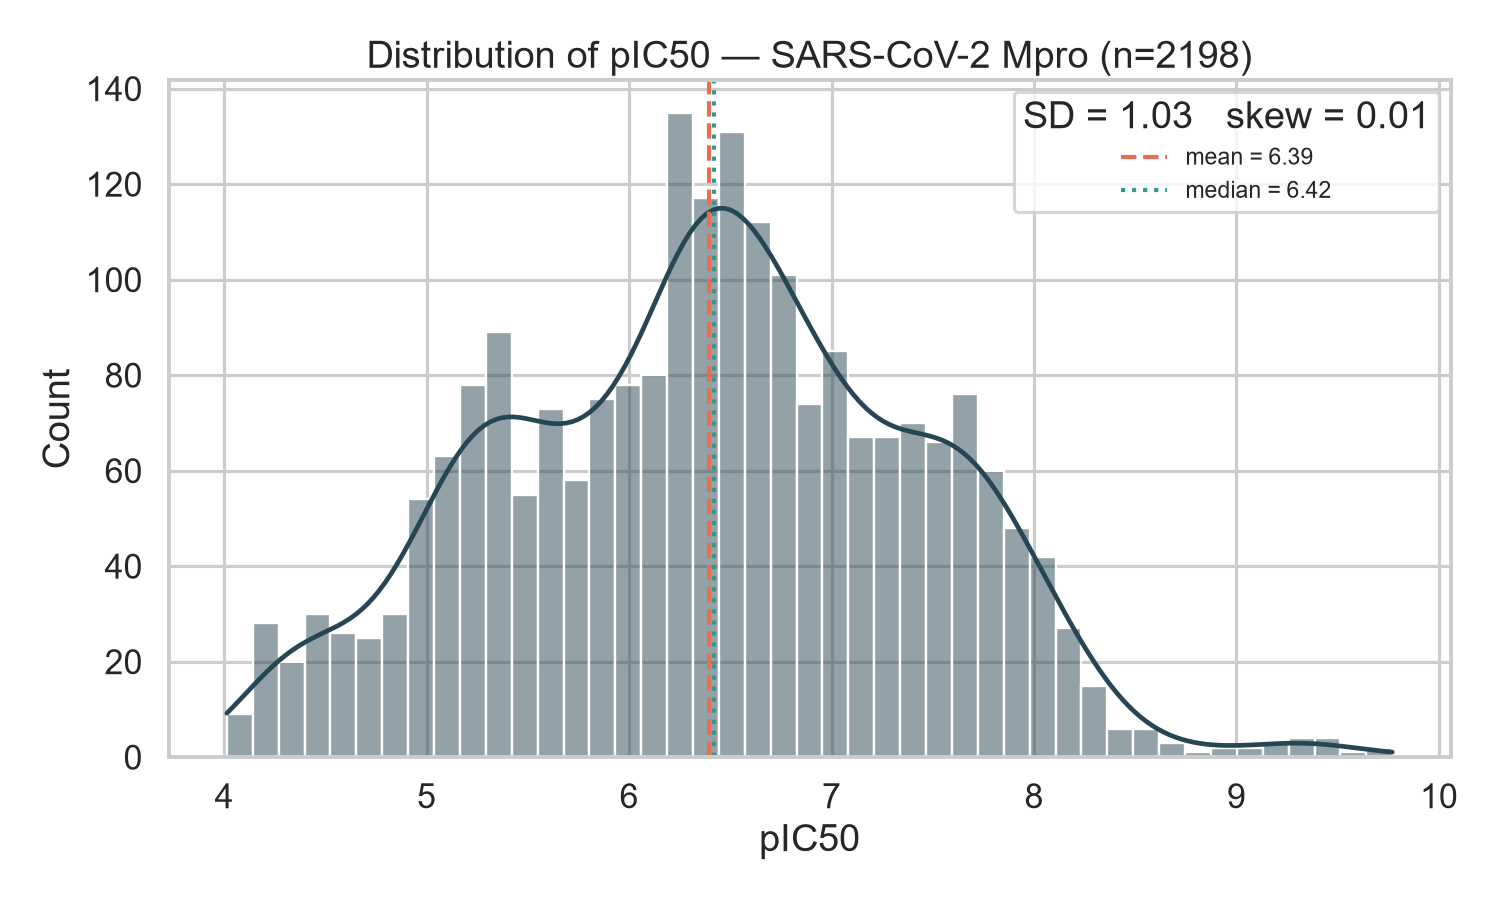
\includegraphics[width=0.86\textwidth]{../figures/fig01_pic50_distribution.png}
\caption{การแจกแจงความถี่ของค่า \pICfifty\ ในชุดข้อมูลหลัก}
\label{fig:pic50dist}
\end{figure}

\begin{figure}[H]
\centering
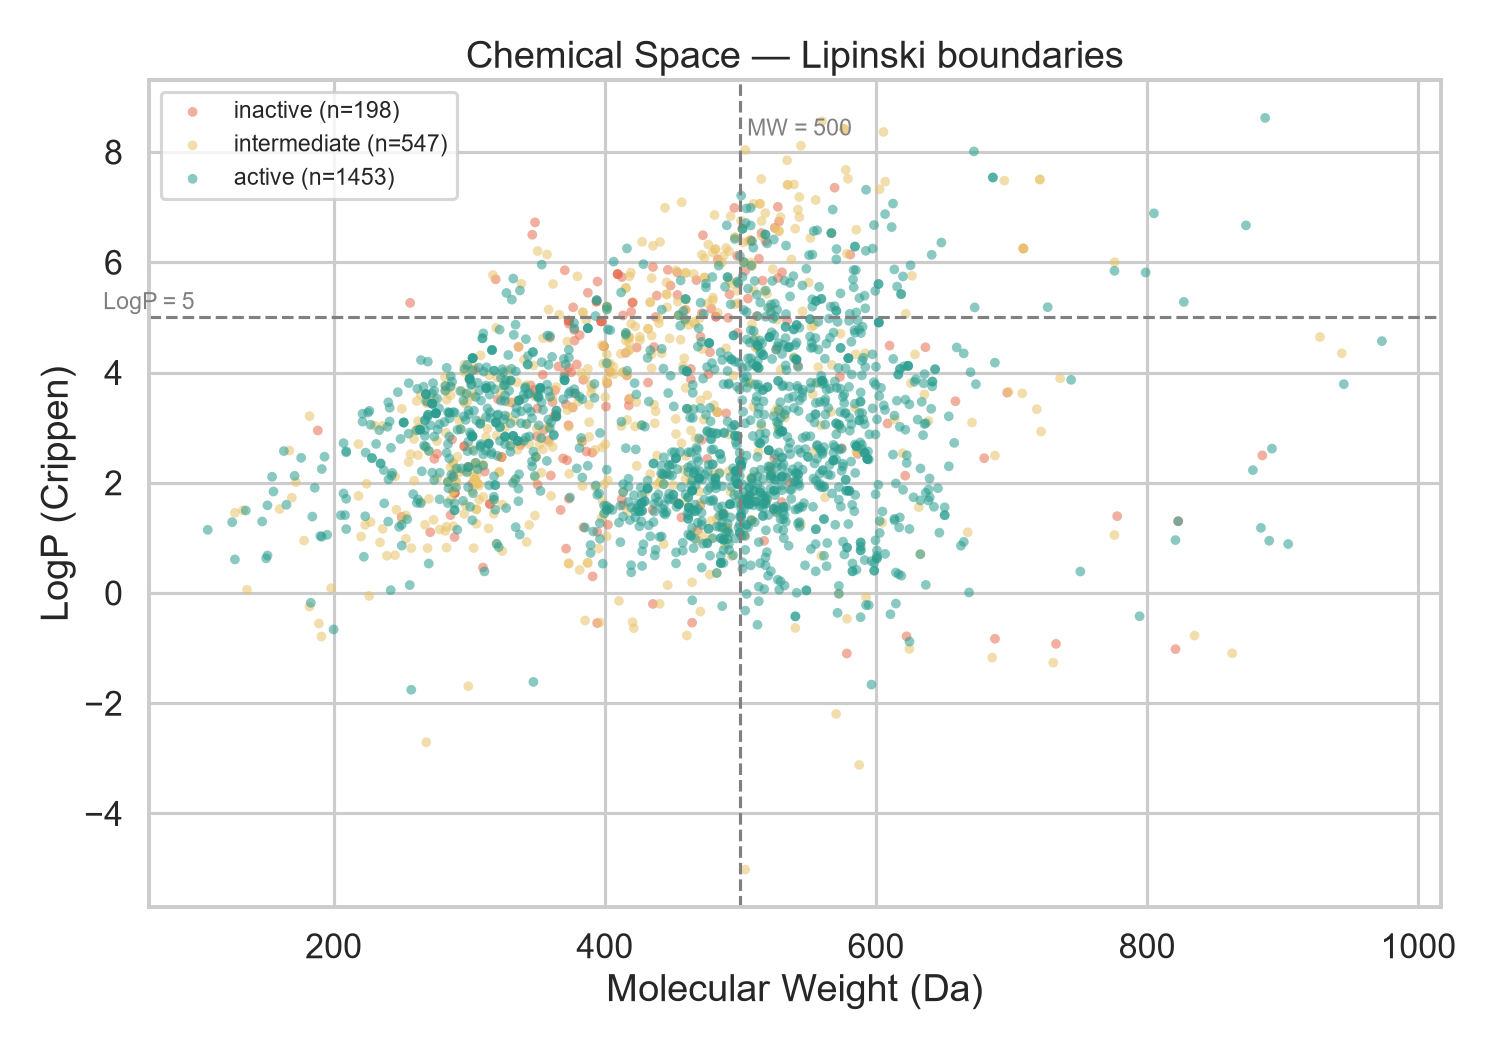
\includegraphics[width=0.82\textwidth]{../figures/fig02_chemical_space_mw_logp.png}
\caption{ปริภูมิเคมีระหว่างน้ำหนักโมเลกุลกับค่า LogP แยกตามกลุ่มฤทธิ์}
\label{fig:chemspace}
\end{figure}

\begin{figure}[H]
\centering
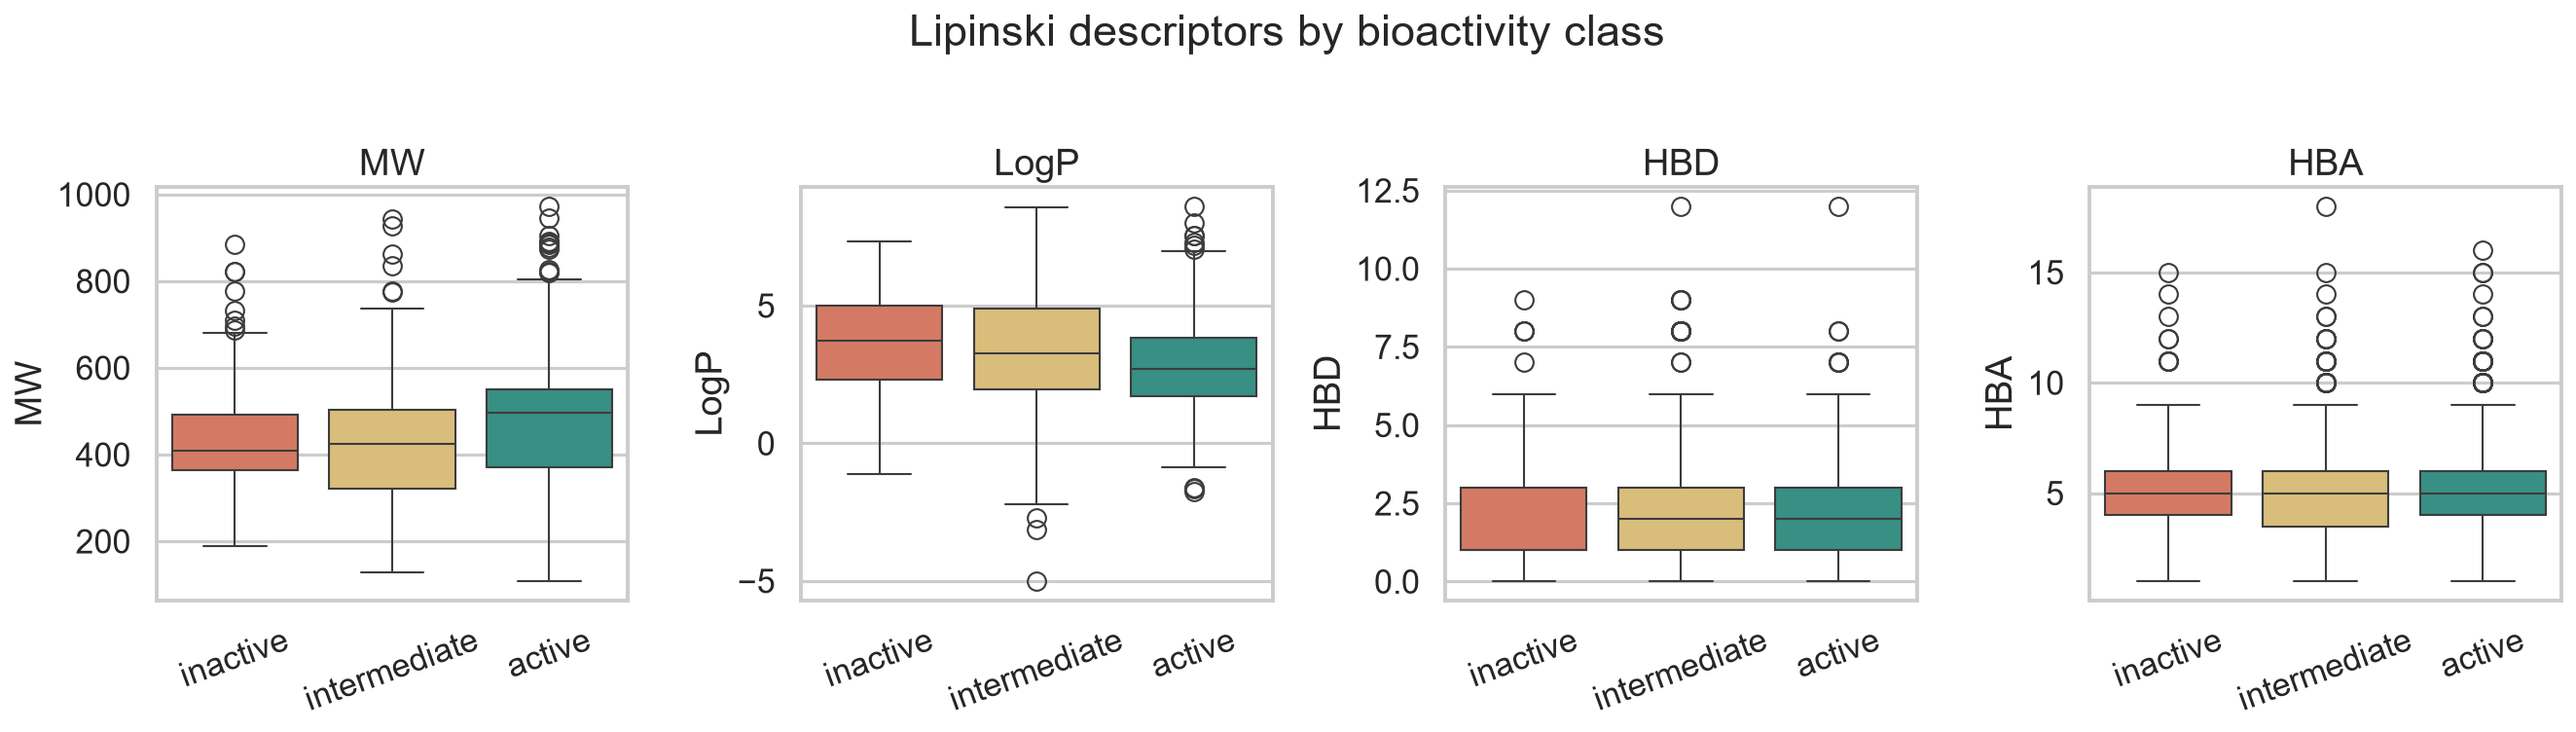
\includegraphics[width=\textwidth]{../figures/fig02b_lipinski_by_class.png}
\caption{การเปรียบเทียบ Lipinski Descriptors ตามกลุ่มฤทธิ์}
\label{fig:lipinskibox}
\end{figure}

\begin{figure}[H]
\centering
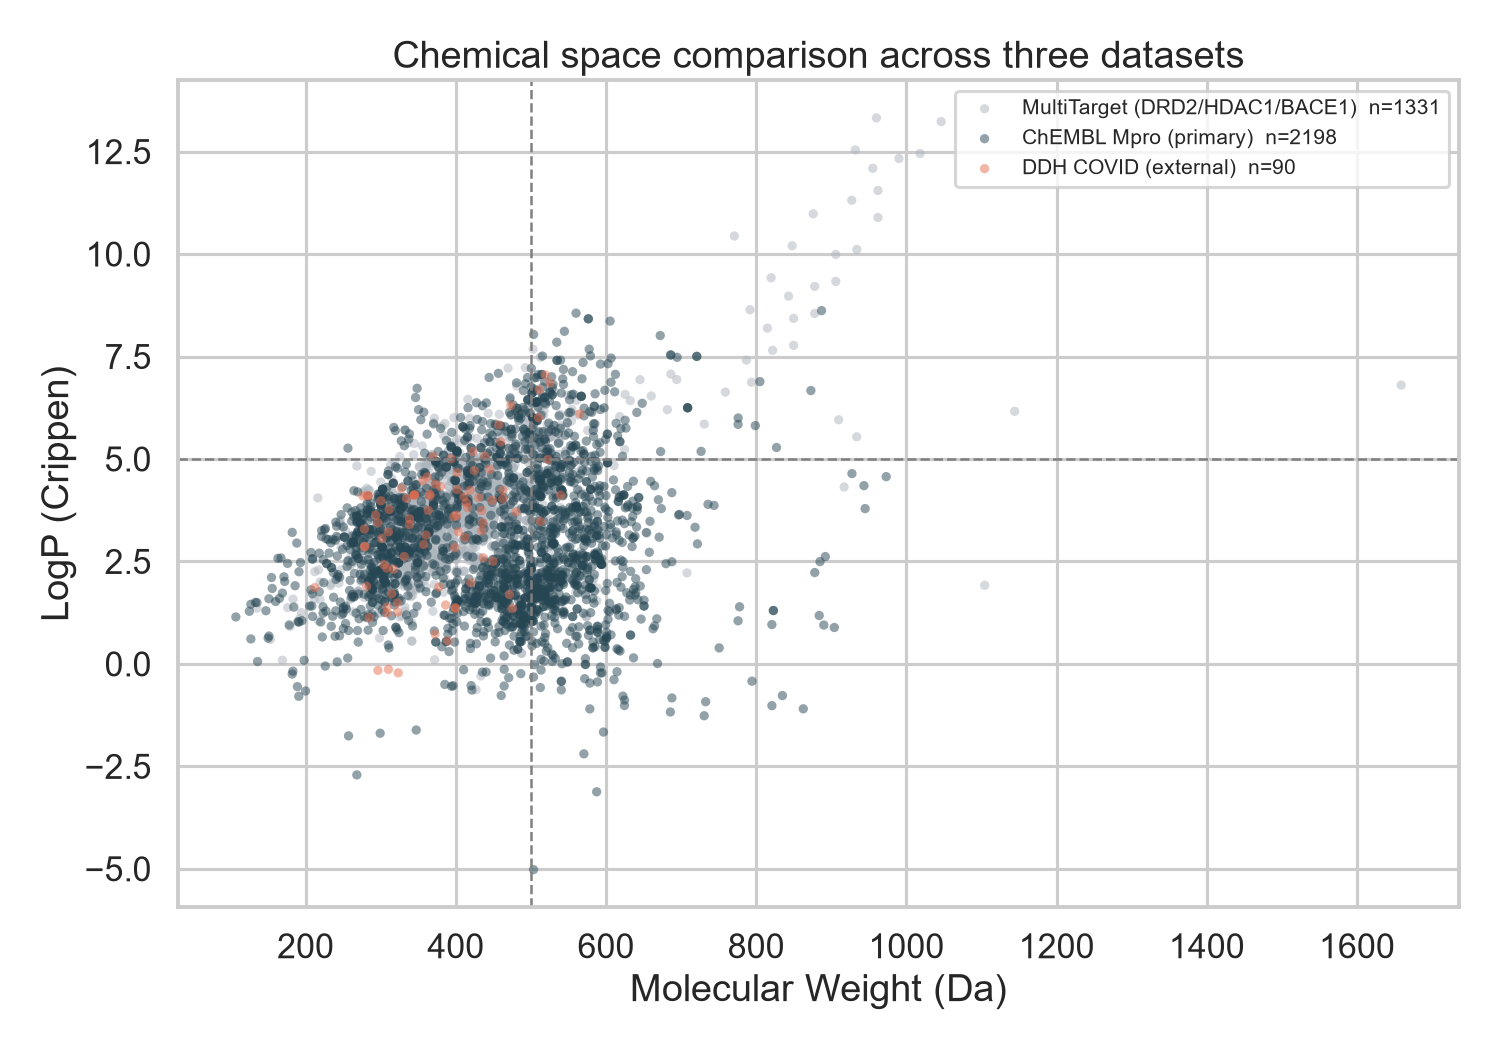
\includegraphics[width=0.82\textwidth]{../figures/fig02c_chemspace_3sets.png}
\caption{การเปรียบเทียบปริภูมิเคมีของชุดข้อมูลสามชุด}
\label{fig:chemspace3}
\end{figure}

\begin{table}[H]
\centering
\caption{โครงสร้างแกนกลาง Murcko 10 อันดับแรก}
\label{tab:scaffolds}
\small
\begin{tabular}{C{1.2cm} L{9.2cm} R{1.8cm} R{1.6cm}}
\toprule
\textbf{อันดับ} & \textbf{Murcko Scaffold} & \textbf{จำนวน} & \textbf{ร้อยละ}\\
\midrule
1 & \texttt{O=C(Oc1cccnc1)c1ccccc1} & 46 & 2.09\\
2 & \texttt{c1ccccc1} & 35 & 1.59\\
3 & \texttt{O=C(c1ccccc1)n1cnc2ccccc21} & 30 & 1.36\\
4 & \texttt{O=c1c2ccccc2[se]n1-c1ccccc1} & 29 & 1.32\\
5 & \texttt{O=c1[nH]c(-c2ccccc2)nc2ccccc12} & 27 & 1.23\\
6 & \texttt{O=C(Cn1sc2ccccc2c1=O)Nc1ccccc1} & 27 & 1.23\\
7 & \texttt{O=C(NCc1ccccc1)C(Nc1ccc(-c2ccccc2)cc1)c1cccnc1} & 27 & 1.23\\
8 & \texttt{O=C1NCCC1CCNC(=O)C1C2CC2CN1C(=O)c1cc2ccccc2[nH]1} & 25 & 1.14\\
9 & \texttt{O=C(NC(Cc1ccccc1)C(=O)NNCc1ccccc1)OCc1ccccc1} & 23 & 1.05\\
10 & \texttt{c1ccc(-c2cccc3c2CCc2c(-c4ccccn4)cccc2-3)cc1} & 22 & 1.00\\
\bottomrule
\end{tabular}
\end{table}

ไม่มี Scaffold ใดที่ครองสัดส่วนเกินร้อยละ 2.1 ซึ่งยืนยันความหลากหลายของชุดข้อมูลอีกครั้ง Scaffold อันดับ 8 มีลักษณะเป็นโครงสร้างเปปไทด์คล้าย ซึ่งสอดคล้องกับสารยับยั้ง \Mpro\ กลุ่มหลักที่พัฒนากันอยู่

\begin{table}[H]
\centering
\caption{การเปรียบเทียบ Lipinski Descriptors ด้วย Mann-Whitney U (active เทียบ inactive)}
\label{tab:mannwhitney}
\begin{tabular}{L{2.8cm} R{3.0cm} R{3.0cm} R{2.3cm} R{2.3cm}}
\toprule
\textbf{Descriptor} & \textbf{มัธยฐาน active} & \textbf{มัธยฐาน inactive} & \textbf{สถิติ U} & \textbf{ค่า p}\\
\midrule
MW & 496.39 & 409.49 & 177{,}509.5 & $8.85\times10^{-8}$\\
LogP & 2.710 & 3.725 & 106{,}106.5 & $2.01\times10^{-9}$\\
HBD & 2.00 & 1.00 & 165{,}977.5 & $3.38\times10^{-4}$\\
HBA & 5.00 & 5.00 & 160{,}018.5 & $8.86\times10^{-3}$\\
\bottomrule
\end{tabular}
\end{table}

ทุก descriptor แตกต่างกันอย่างมีนัยสำคัญทางสถิติที่ระดับ 0.01 โดยพบรูปแบบที่ชัดเจนคือ สารกลุ่ม active มี \textbf{น้ำหนักโมเลกุลสูงกว่า} (มัธยฐาน 496 เทียบกับ 409 Da) และ \textbf{ค่า LogP ต่ำกว่า} (2.71 เทียบกับ 3.73) สารกลุ่ม inactive อย่างมีนัยสำคัญ

รูปแบบนี้สอดคล้องกับความรู้ทางเคมียาที่ว่า สารยับยั้ง \Mpro\ ที่มีประสิทธิภาพมักเป็นโมเลกุลขนาดใหญ่ที่มีลักษณะคล้ายเปปไทด์ มีขั้วค่อนข้างสูง และมีหมู่ที่สร้างพันธะไฮโดรเจนกับกรดอะมิโนในช่องจับของเอนไซม์ได้ดี สังเกตได้จากค่า HBD ที่สูงกว่า อย่างไรก็ตาม น้ำหนักโมเลกุลมัธยฐานของสาร active ที่ 496 Da นั้นเกือบชนขีดจำกัดของกฎลิพินสกีที่ 500 Da ซึ่งสะท้อนความท้าทายในการพัฒนาสารกลุ่มนี้ให้เป็นยารับประทาน

\section{ผลการทำ Cross-Validation}

การแบ่งข้อมูลได้ผลดังนี้ Random Split ให้ชุดฝึก 1{,}648 โมเลกุลและชุดทดสอบ 550 โมเลกุล ส่วน Scaffold Split ให้ชุดฝึก 1{,}649 โมเลกุลและชุดทดสอบ 549 โมเลกุล

\begin{table}[H]
\centering
\caption{ผล 5-Fold Cross-Validation บนชุดฝึก Random Split (E1)}
\label{tab:cve1}
\small
\begin{tabular}{L{3.2cm} C{2.8cm} R{1.7cm} R{1.7cm} R{1.7cm} R{1.7cm}}
\toprule
\textbf{แบบจำลอง} & \textbf{CV \Rsq\ (เฉลี่ย $\pm$ SD)} & \textbf{RMSE} & \textbf{MAE} & \textbf{Train \Rsq} & \textbf{Gap}\\
\midrule
Dummy Regressor & $-0.0021 \pm 0.0013$ & 1.0371 & 0.8395 & 0.0000 & 0.0021\\
\textbf{Random Forest} & $\mathbf{0.5997 \pm 0.0394}$ & \textbf{0.6544} & 0.4481 & 0.9368 & 0.3371\\
XGBoost & $0.5803 \pm 0.0342$ & 0.6707 & 0.4531 & 0.9573 & 0.3770\\
SVR (RBF) & $0.5994 \pm 0.0461$ & 0.6549 & \textbf{0.4433} & 0.9703 & 0.3709\\
\bottomrule
\end{tabular}
\end{table}

\begin{table}[H]
\centering
\caption{ผล 5-Fold Cross-Validation บนชุดฝึก Scaffold Split (E2)}
\label{tab:cve2}
\small
\begin{tabular}{L{3.2cm} C{2.8cm} R{1.7cm} R{1.7cm} R{1.7cm} R{1.7cm}}
\toprule
\textbf{แบบจำลอง} & \textbf{CV \Rsq\ (เฉลี่ย $\pm$ SD)} & \textbf{RMSE} & \textbf{MAE} & \textbf{Train \Rsq} & \textbf{Gap}\\
\midrule
Dummy Regressor & $-0.0037 \pm 0.0019$ & 1.0204 & 0.8173 & 0.0000 & 0.0037\\
Random Forest & $0.6670 \pm 0.0181$ & 0.5876 & 0.3993 & 0.9407 & 0.2736\\
XGBoost & $0.6527 \pm 0.0127$ & 0.6002 & 0.4035 & 0.9515 & 0.2988\\
\textbf{SVR (RBF)} & $\mathbf{0.6735 \pm 0.0132}$ & \textbf{0.5820} & \textbf{0.3911} & 0.9609 & 0.2875\\
\bottomrule
\end{tabular}
\end{table}

ในระยะ Cross-Validation แบบจำลองทั้งสามที่ไม่ใช่ Dummy ให้ผลใกล้เคียงกันมาก โดย Random Forest นำเล็กน้อยในกรณี Random Split ค่า Dummy Regressor ที่ได้ \Rsq\ ติดลบเล็กน้อยเป็นไปตามที่คาดในทางทฤษฎี

ส่วนต่างระหว่าง Train \Rsq\ กับ CV \Rsq\ อยู่ในช่วง 0.27--0.38 ในทุกแบบจำลอง แสดงว่ามีการเรียนรู้เกินอยู่พอสมควร โดยเฉพาะ SVR ที่มี Train \Rsq\ สูงถึง 0.9703 ซึ่งเป็นลักษณะปกติของแบบจำลองที่ทำงานบนคุณลักษณะมิติสูง

\begin{table}[H]
\centering
\caption{ผลการศึกษา Ablation}
\label{tab:ablation}
\begin{tabular}{C{1.6cm} L{5.0cm} R{2.3cm} R{2.1cm} R{2.1cm}}
\toprule
\textbf{การทดลอง} & \textbf{คุณลักษณะ} & \textbf{จำนวนมิติ} & \textbf{CV \Rsq} & \textbf{CV RMSE}\\
\midrule
E4 & Lipinski เท่านั้น & 4 & 0.2668 & 0.8875\\
E3 & Morgan FP เท่านั้น & 1{,}024 & 0.5885 & 0.6636\\
\textbf{E1} & \textbf{Hybrid (FP + Lipinski)} & \textbf{1{,}028} & \textbf{0.5997} & \textbf{0.6544}\\
\bottomrule
\end{tabular}
\end{table}

ผลการศึกษา Ablation แสดงว่าคุณลักษณะแบบผสมให้ผลดีที่สุด โดยดีกว่าการใช้ Morgan FP อย่างเดียว $+0.0112$ \Rsq\ และดีกว่าการใช้ Lipinski อย่างเดียว $+0.3329$ \Rsq

\begin{keynote}
พลังการทำนายส่วนใหญ่มาจาก Morgan Fingerprints ขณะที่ Lipinski Descriptors เพิ่มค่าเพียงเล็กน้อย อย่างไรก็ตาม การเพิ่มขึ้น 0.0112 \Rsq\ จากการเพิ่มคุณลักษณะเพียง 4 มิติ คิดเป็นร้อยละ 0.39 ของจำนวนมิติทั้งหมด ถือว่าคุ้มค่าในเชิงอัตราส่วนต้นทุนต่อผลตอบแทน
\end{keynote}

\begin{table}[H]
\centering
\caption{ผลการพิสูจน์ Data Leakage}
\label{tab:leakage}
\begin{tabular}{C{1.6cm} L{7.2cm} R{2.3cm} R{2.3cm}}
\toprule
\textbf{การทดลอง} & \textbf{กรณี} & \textbf{CV \Rsq} & \textbf{ส่วนต่าง}\\
\midrule
E5 & A ถูกต้อง --- ปรับสเกลภายใน Pipeline & 0.5994 & ---\\
E5 & B ผิด --- ปรับสเกลก่อนแบ่งข้อมูล & 0.5995 & $\mathbf{+0.0001}$\\
\midrule
E5b & A ถูกต้อง --- SelectKBest ภายใน Pipeline & 0.5892 & ---\\
E5b & B ผิด --- SelectKBest บนข้อมูลทั้งชุด & 0.6008 & $\mathbf{+0.0116}$\\
\bottomrule
\end{tabular}
\end{table}

ผลการทดลองนี้เป็นข้อค้นพบที่ต้องรายงานอย่างตรงไปตรงมา เนื่องจากไม่เป็นไปตามที่คาดการณ์ไว้ล่วงหน้า

\textbf{การทดลอง E5 แสดงว่า Preprocessing Leakage แทบไม่มีผลเลย} ส่วนต่างเพียง $+0.0001$ \Rsq\ อธิบายได้จากสองเหตุผล ประการแรก มีเพียง 4 คุณลักษณะจากทั้งหมด 1{,}028 คุณลักษณะที่ผ่านการปรับสเกล คิดเป็นร้อยละ 0.39 เท่านั้น ประการที่สอง ขนาดชุดฝึก 1{,}648 ตัวอย่างมีขนาดใหญ่เพียงพอที่ค่าเฉลี่ยและส่วนเบี่ยงเบนมาตรฐานที่คำนวณจากชุดฝึกของแต่ละ Fold แทบไม่ต่างจากที่คำนวณจากข้อมูลทั้งชุด

\textbf{การทดลอง E5b แสดงว่า Feature Selection Leakage ให้อคติบวกที่วัดได้จริง} ส่วนต่าง $+0.0116$ \Rsq\ ซึ่งมากกว่า E5 ถึง 116 เท่า การรั่วไหลรูปแบบนี้ตรงกับสิ่งที่ตรวจพบในไฟล์ \texttt{xfinal.csv} ที่ได้รับมอบมา ซึ่งคัดเลือกคุณลักษณะ 300 ตัวจาก 4{,}262 คอลัมน์บนข้อมูลทั้งชุด ผลการทดลองนี้จึงเป็นหลักฐานเชิงประจักษ์ที่สนับสนุนการตัดสินใจไม่ใช้ไฟล์ดังกล่าว

\section{ผลการปรับจูนและประเมินบนชุดทดสอบ}

\begin{table}[H]
\centering
\caption{ไฮเปอร์พารามิเตอร์ที่ดีที่สุด (Random Split)}
\label{tab:bestparams}
\small
\begin{tabular}{L{3.0cm} L{10.6cm}}
\toprule
\textbf{แบบจำลอง} & \textbf{ค่าที่เลือกได้}\\
\midrule
Random Forest & \texttt{n\_estimators}=500, \texttt{max\_depth}=None, \texttt{min\_samples\_split}=5, \texttt{min\_samples\_leaf}=1, \texttt{max\_features}=0.3\\
XGBoost & \texttt{n\_estimators}=600, \texttt{learning\_rate}=0.03, \texttt{max\_depth}=8, \texttt{subsample}=0.8, \texttt{colsample\_bytree}=0.6\\
SVR (RBF) & \texttt{C}=1, \texttt{gamma}='scale', \texttt{epsilon}=0.05\\
\bottomrule
\end{tabular}
\end{table}

\begin{table}[H]
\centering
\caption{ผลการประเมินบนชุดทดสอบ Random Split ($n = 550$)}
\label{tab:testrandom}
\begin{tabular}{L{3.4cm} R{2.2cm} R{2.2cm} R{2.2cm} R{2.4cm}}
\toprule
\textbf{แบบจำลอง} & \textbf{\Rsq} & \textbf{RMSE} & \textbf{MAE} & \textbf{Spearman $\rho$}\\
\midrule
Dummy Regressor & $-0.0000$ & 1.0074 & 0.8054 & ---\\
Random Forest & 0.6822 & 0.5679 & 0.4107 & 0.8351\\
\textbf{XGBoost} & $\mathbf{0.7034}$ & $\mathbf{0.5487}$ & $\mathbf{0.3918}$ & $\mathbf{0.8415}$\\
SVR (RBF) & 0.6716 & 0.5774 & 0.4199 & 0.8257\\
\bottomrule
\end{tabular}
\end{table}

\begin{table}[H]
\centering
\caption{ผลการประเมินบนชุดทดสอบ Scaffold Split ($n = 549$)}
\label{tab:testscaffold}
\begin{tabular}{L{3.4cm} R{2.2cm} R{2.2cm} R{2.2cm} R{2.4cm}}
\toprule
\textbf{แบบจำลอง} & \textbf{\Rsq} & \textbf{RMSE} & \textbf{MAE} & \textbf{Spearman $\rho$}\\
\midrule
Dummy Regressor & $-0.0162$ & 1.0611 & 0.8715 & ---\\
Random Forest & 0.4949 & 0.7481 & 0.5626 & 0.7414\\
\textbf{XGBoost} & $\mathbf{0.5127}$ & $\mathbf{0.7348}$ & $\mathbf{0.5440}$ & $\mathbf{0.7452}$\\
SVR (RBF) & 0.4637 & 0.7708 & 0.5866 & 0.7057\\
\bottomrule
\end{tabular}
\end{table}

\textbf{XGBoost ให้ผลดีที่สุดบนชุดทดสอบทั้งสองวิธีการแบ่ง} ซึ่งน่าสนใจเพราะในระยะ Cross-Validation ก่อนปรับจูน XGBoost ทำได้ต่ำที่สุดในสามแบบจำลอง ผลนี้แสดงว่า XGBoost ได้ประโยชน์จากการปรับจูนไฮเปอร์พารามิเตอร์มากกว่าแบบจำลองอื่น โดยค่าที่เลือกได้คือ \texttt{learning\_rate} ต่ำที่ 0.03 ร่วมกับจำนวนต้นไม้มากที่ 600 ต้น ซึ่งเป็นการแลกความเร็วกับความแม่นยำ

\begin{keynote}[ประเด็นสำคัญที่สุดของบทนี้]
ค่า \Rsq\ ของ XGBoost ลดลงจาก 0.7034 บน Random Split เหลือ 0.5127 บน Scaffold Split คิดเป็นการลดลงร้อยละ 27.1 ส่วนต่างนี้ยืนยันคำเตือนของ Sheridan (2013) ว่าการแบ่งข้อมูลแบบสุ่มให้ค่าที่มองโลกในแง่ดีเกินไป เพราะโมเลกุลในอนุกรมเคมีเดียวกันกระจายอยู่ทั้งสองฝั่ง ในทางปฏิบัติ ตัวเลขที่ควรอ้างอิงเมื่อพูดถึงการทำนายสารที่มีโครงสร้างแกนกลางใหม่คือ $\Rsq = 0.5127$ ไม่ใช่ 0.7034
\end{keynote}

\begin{figure}[H]
\centering
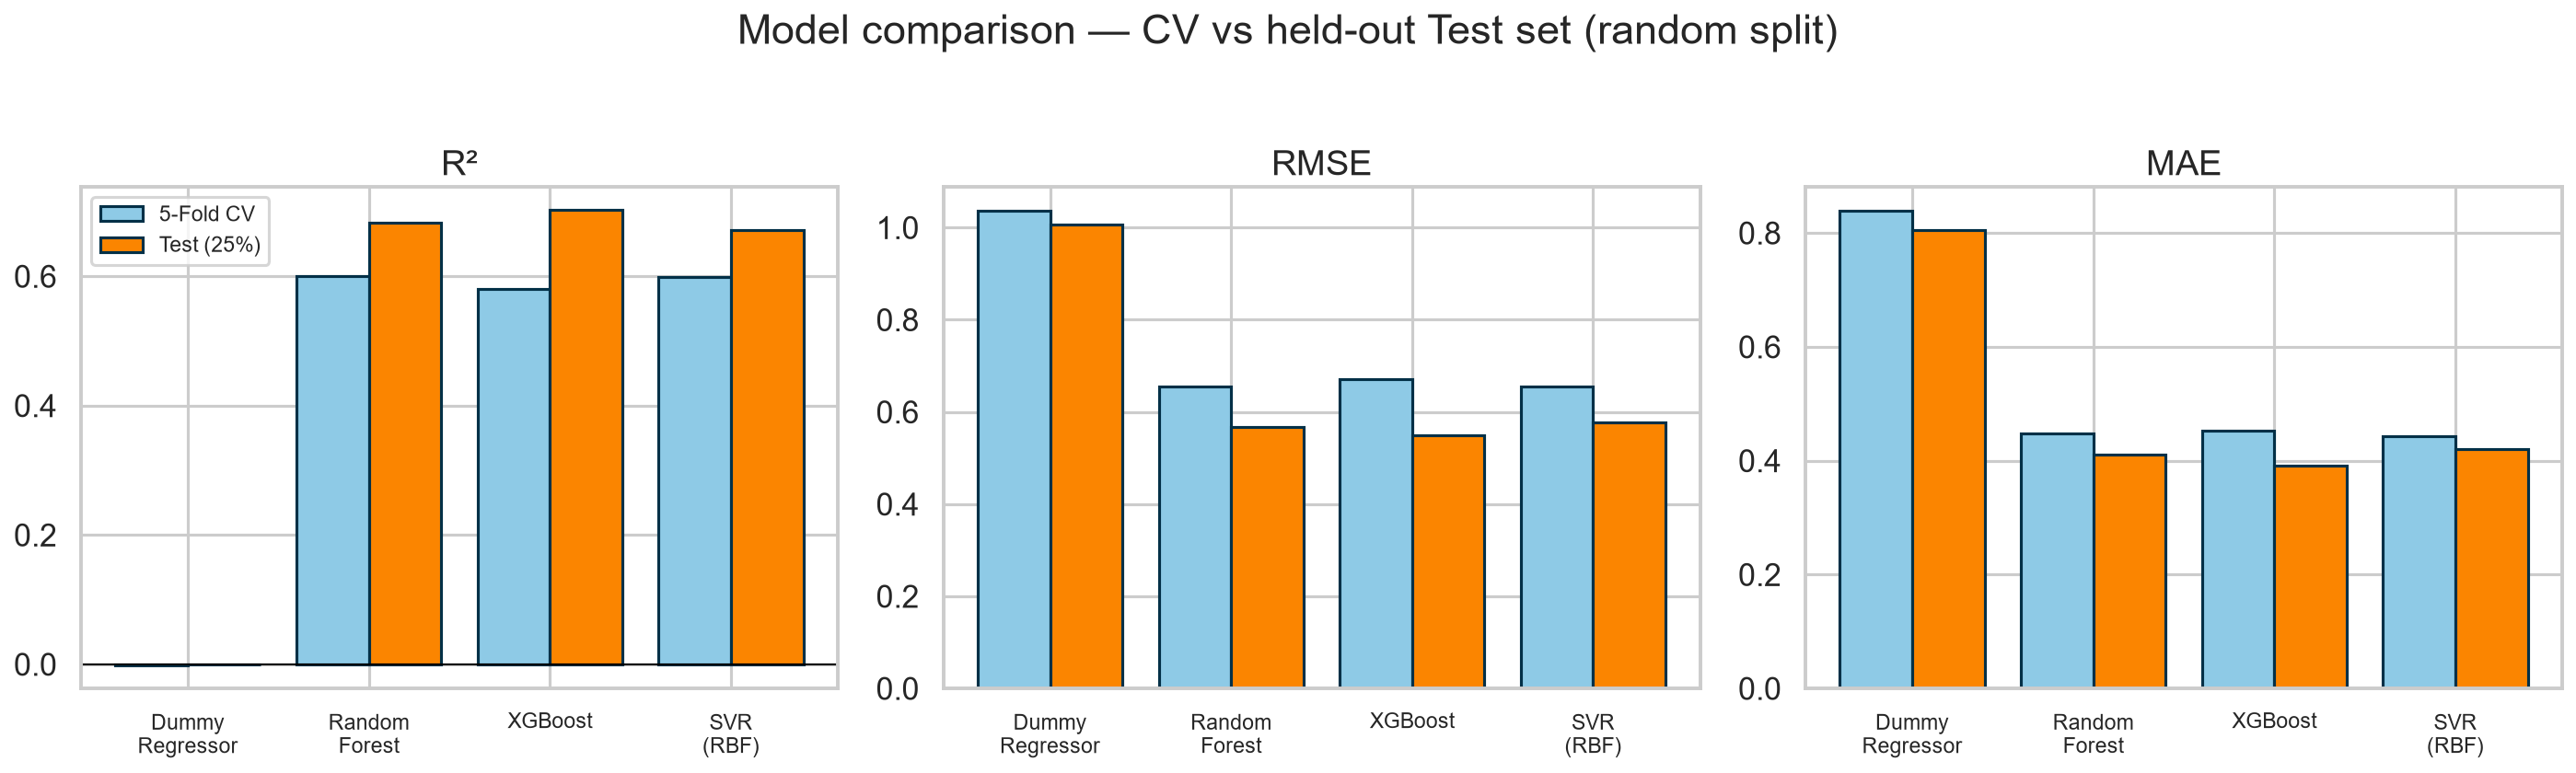
\includegraphics[width=\textwidth]{../figures/fig03_model_comparison.png}
\caption{การเปรียบเทียบประสิทธิภาพแบบจำลองระหว่าง Cross-Validation กับชุดทดสอบ}
\label{fig:modelcomp}
\end{figure}

\section{การวิเคราะห์ค่าคลาดเคลื่อน}

ค่าคลาดเคลื่อนโดยรวมของแบบจำลอง XGBoost บนชุดทดสอบ Random Split มีค่าเฉลี่ย $-0.0368$ และส่วนเบี่ยงเบนมาตรฐาน 0.5479 log unit การทำนายร้อยละ 93.6 มีความคลาดเคลื่อนไม่เกิน 1 log unit และร้อยละ 72.5 ไม่เกิน 0.5 log unit

\begin{figure}[H]
\centering
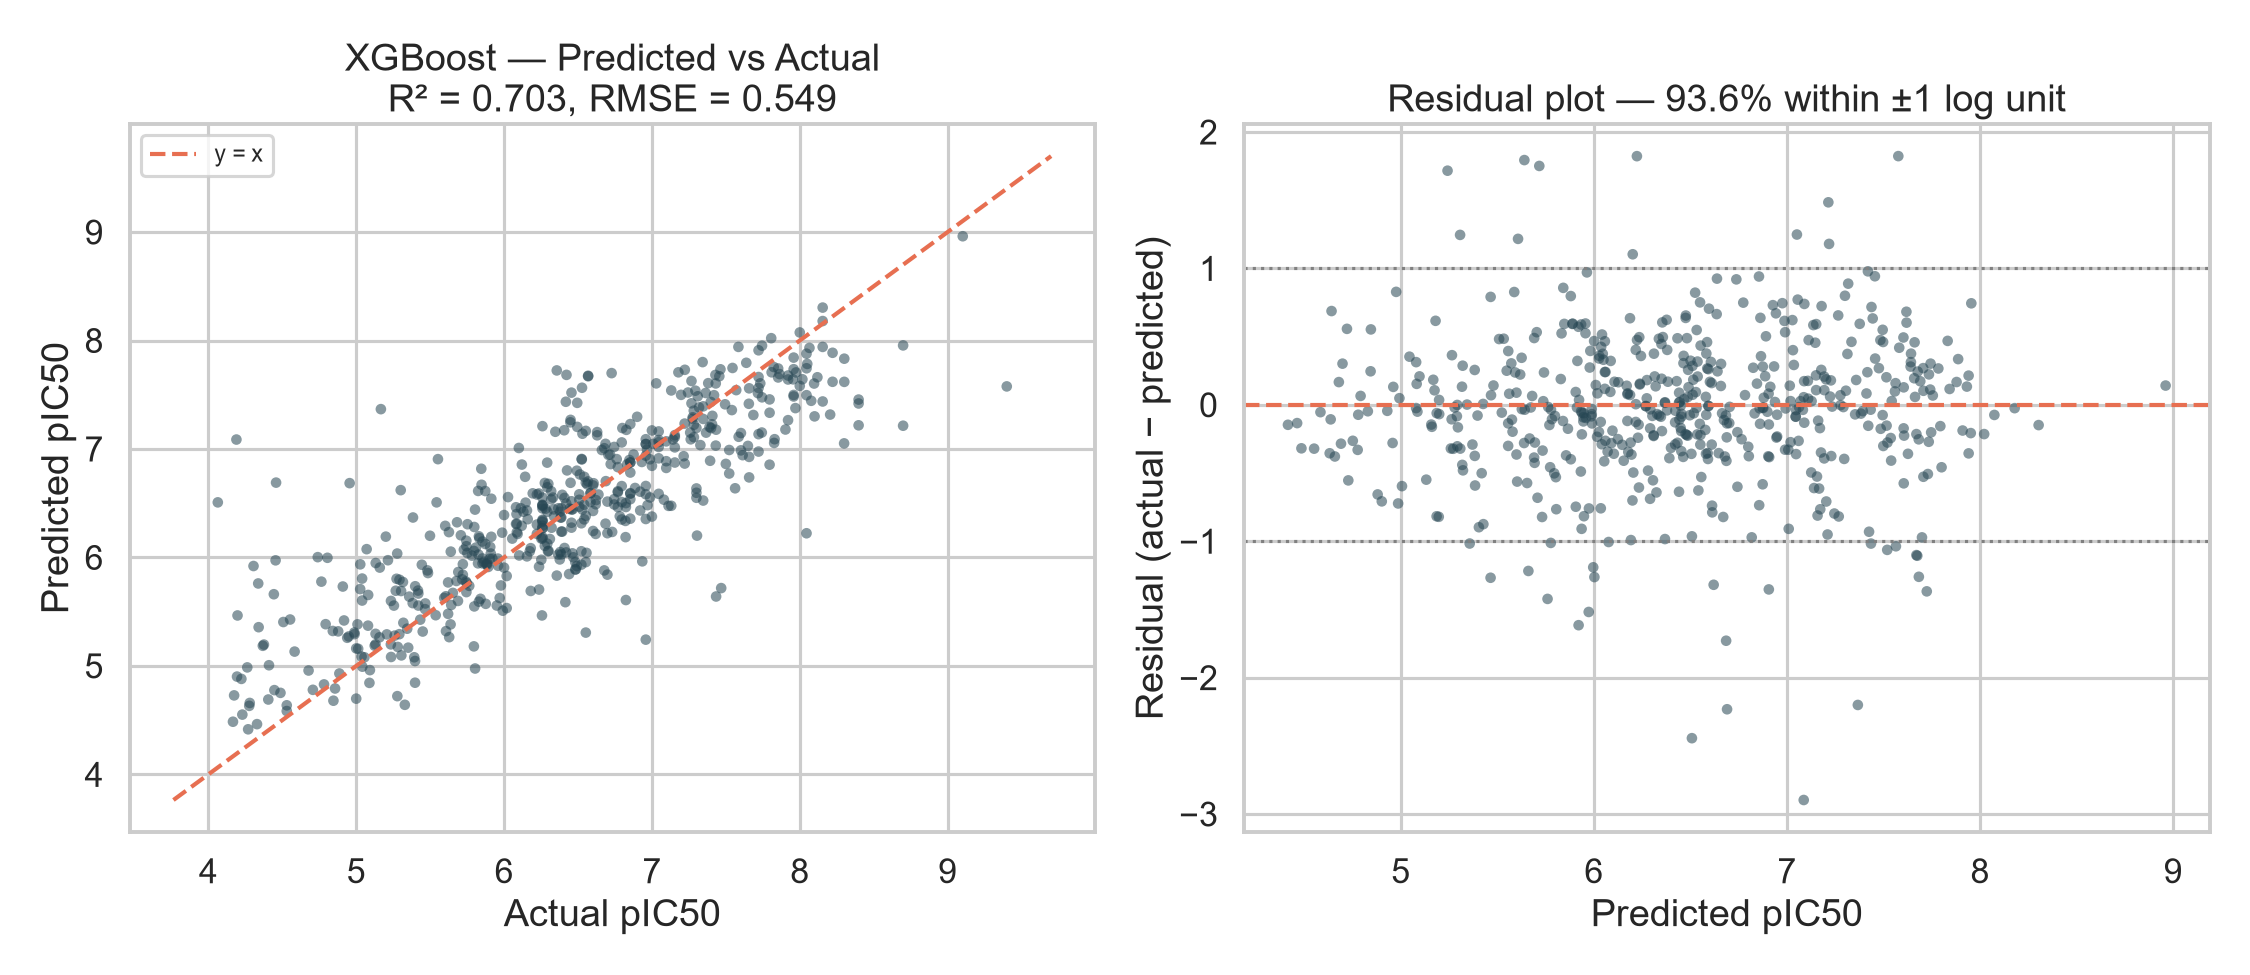
\includegraphics[width=\textwidth]{../figures/fig04_residual_plot.png}
\caption{กราฟค่าทำนายเทียบค่าจริง (ซ้าย) และกราฟค่าคลาดเคลื่อน (ขวา)}
\label{fig:residual}
\end{figure}

\begin{figure}[H]
\centering
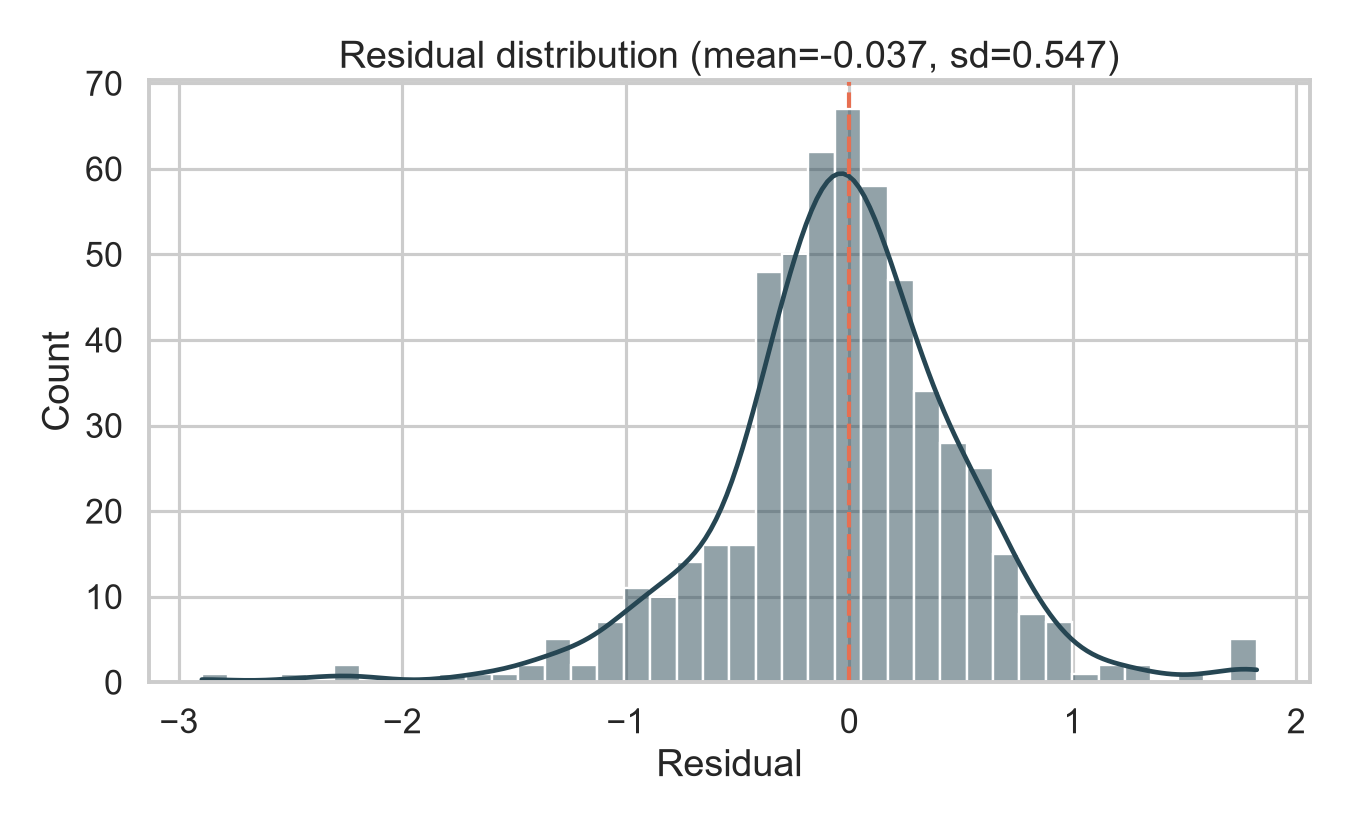
\includegraphics[width=0.76\textwidth]{../figures/fig04b_residual_hist.png}
\caption{การแจกแจงค่าคลาดเคลื่อน}
\label{fig:residualhist}
\end{figure}

\begin{table}[H]
\centering
\caption{การวิเคราะห์ค่าคลาดเคลื่อนแยกตามกลุ่มฤทธิ์}
\label{tab:residualclass}
\begin{tabular}{L{3.4cm} R{2.0cm} R{3.4cm} R{2.2cm} R{2.2cm}}
\toprule
\textbf{กลุ่มฤทธิ์} & \textbf{จำนวน} & \textbf{ค่าคลาดเคลื่อนเฉลี่ย} & \textbf{MAE} & \textbf{RMSE}\\
\midrule
active & 364 & $+0.1203$ & 0.3635 & 0.4926\\
intermediate & 137 & $-0.2116$ & 0.3481 & 0.4790\\
\textbf{inactive} & \textbf{49} & $\mathbf{-0.7151}$ & \textbf{0.7246} & \textbf{0.9667}\\
\bottomrule
\end{tabular}
\end{table}

ผลการวิเคราะห์นี้เปิดเผยจุดอ่อนสำคัญของแบบจำลอง กล่าวคือ \textbf{แบบจำลองทำนายสารกลุ่ม inactive สูงเกินจริงอย่างเป็นระบบเฉลี่ย 0.72 log unit} และมีค่า RMSE สูงถึง 0.9667 เกือบสองเท่าของอีกสองกลุ่ม

สาเหตุมาจากความไม่สมดุลของชุดข้อมูลฝึก ซึ่งมีสาร active ถึง 1{,}453 ตัว แต่มี inactive เพียง 198 ตัว คิดเป็นอัตราส่วน 7.3 ต่อ 1 แบบจำลองจึงมีแนวโน้มเอนเอียงไปทางการทำนายค่าสูง

ค่าคลาดเคลื่อนที่มากที่สุดสามอันดับแรกล้วนเป็นสารกลุ่ม inactive ที่ถูกทำนายเป็น active ได้แก่ ค่าจริง 4.190 ทำนาย 7.087 (คลาดเคลื่อน $-2.897$), ค่าจริง 4.064 ทำนาย 6.508 (คลาดเคลื่อน $-2.444$) และค่าจริง 4.458 ทำนาย 6.690 (คลาดเคลื่อน $-2.232$)

ข้อค้นพบนี้มีนัยสำคัญเชิงปฏิบัติ เพราะในงานคัดกรองยา การทำนายสารที่ไม่มีฤทธิ์ว่ามีฤทธิ์ (False Positive) จะทำให้เสียทรัพยากรไปกับการทดสอบสารที่ไม่มีประโยชน์

\section{ผลการวิเคราะห์ SHAP และ SAR}

แบบจำลองที่ใช้วิเคราะห์คือ XGBoost ซึ่งเป็นแบบจำลองประเภทต้นไม้ที่ให้ผลดีที่สุด คำนวณค่า SHAP บนชุดทดสอบ 400 โมเลกุล

\begin{table}[H]
\centering
\caption{ค่าความสำคัญของคุณลักษณะ 20 อันดับแรก}
\label{tab:shapimp}
\small
\begin{tabular}{C{1.4cm} L{2.6cm} R{2.6cm} L{4.6cm}}
\toprule
\textbf{อันดับ} & \textbf{คุณลักษณะ} & \textbf{Mean$|$SHAP$|$} & \textbf{ประเภท}\\
\midrule
1 & \textbf{MW} & \textbf{0.1165} & \textbf{Lipinski descriptor}\\
2 & FP\_10 & 0.0561 & Morgan fingerprint bit\\
3 & FP\_904 & 0.0557 & Morgan fingerprint bit\\
4 & FP\_301 & 0.0484 & Morgan fingerprint bit\\
5 & \textbf{HBA} & \textbf{0.0392} & \textbf{Lipinski descriptor}\\
6 & FP\_847 & 0.0365 & Morgan fingerprint bit\\
7 & FP\_578 & 0.0364 & Morgan fingerprint bit\\
8 & FP\_684 & 0.0361 & Morgan fingerprint bit\\
9 & FP\_807 & 0.0304 & Morgan fingerprint bit\\
10 & FP\_794 & 0.0303 & Morgan fingerprint bit\\
11 & \textbf{LogP} & \textbf{0.0288} & \textbf{Lipinski descriptor}\\
12 & FP\_583 & 0.0277 & Morgan fingerprint bit\\
13 & FP\_675 & 0.0242 & Morgan fingerprint bit\\
14 & FP\_759 & 0.0207 & Morgan fingerprint bit\\
15 & FP\_482 & 0.0196 & Morgan fingerprint bit\\
16 & \textbf{HBD} & \textbf{0.0196} & \textbf{Lipinski descriptor}\\
17 & FP\_206 & 0.0193 & Morgan fingerprint bit\\
18 & FP\_117 & 0.0184 & Morgan fingerprint bit\\
19 & FP\_330 & 0.0180 & Morgan fingerprint bit\\
20 & FP\_305 & 0.0172 & Morgan fingerprint bit\\
\bottomrule
\end{tabular}
\end{table}

\begin{keynote}[ข้อค้นพบที่สำคัญที่สุด]
น้ำหนักโมเลกุลเป็นคุณลักษณะที่มีอิทธิพลสูงสุด โดยมีค่า Mean$|$SHAP$|$ = 0.1165 ซึ่งสูงกว่าบิต Fingerprint ที่ดีที่สุดถึง 2.08 เท่า และ \textbf{Lipinski Descriptors ติดอันดับ 20 แรกครบทั้ง 4 ตัว}
\end{keynote}

ผลนี้ดูขัดแย้งกับผลการศึกษา Ablation ที่พบว่าการเพิ่ม Lipinski เข้าไปเพิ่มค่า \Rsq\ เพียง 0.0112 คำอธิบายคือ Morgan Fingerprints เข้ารหัสข้อมูลเกี่ยวกับขนาดและองค์ประกอบของโมเลกุลไว้โดยอ้อมอยู่แล้ว เพราะโมเลกุลใหญ่ย่อมมีบิตถูกเซ็ตมากกว่า เมื่อตัด Lipinski ออก แบบจำลองจึงสามารถชดเชยด้วยการรวมสารสนเทศจากบิตหลายบิตแทน คุณลักษณะ Lipinski จึง \textbf{สำคัญแต่ซ้ำซ้อน (Important but Redundant)} ซึ่งเป็นสถานการณ์ที่พบได้ทั่วไปเมื่อวิเคราะห์ความสำคัญของคุณลักษณะ

\begin{figure}[H]
\centering
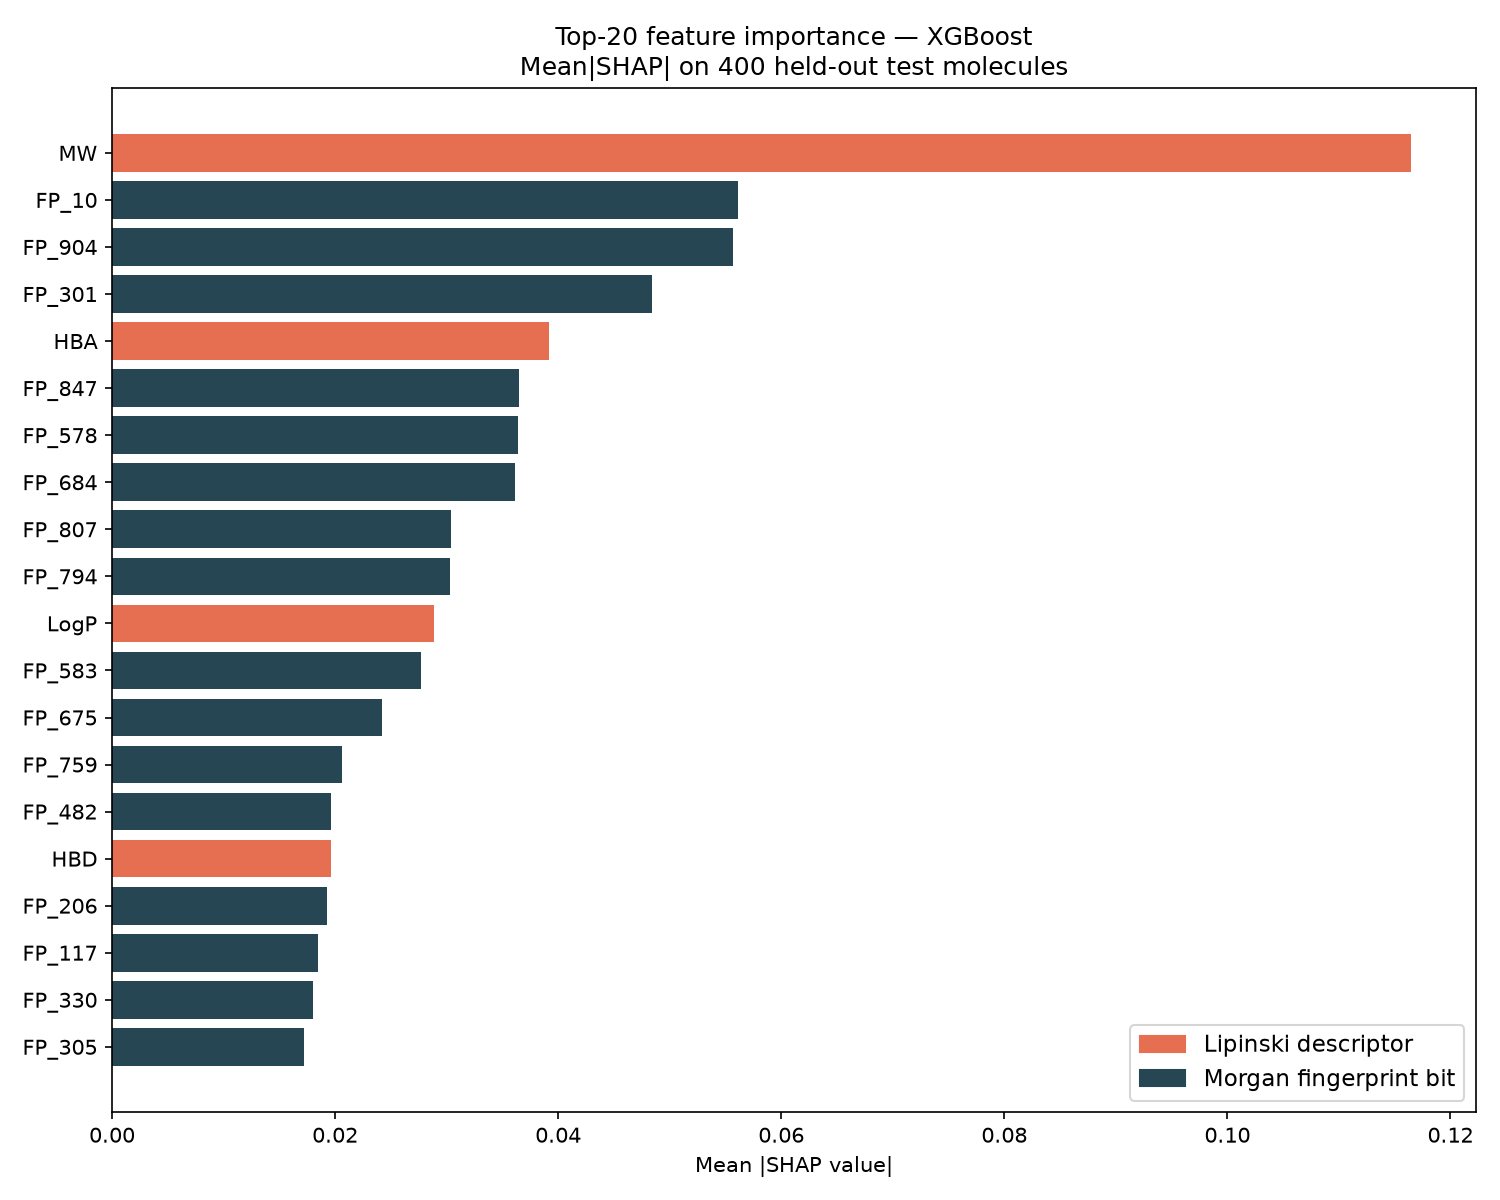
\includegraphics[width=0.80\textwidth]{../figures/fig05_shap_bar_top20.png}
\caption{ค่าความสำคัญของคุณลักษณะ 20 อันดับแรกโดย Mean$|$SHAP$|$}
\label{fig:shapbar}
\end{figure}

\begin{figure}[H]
\centering
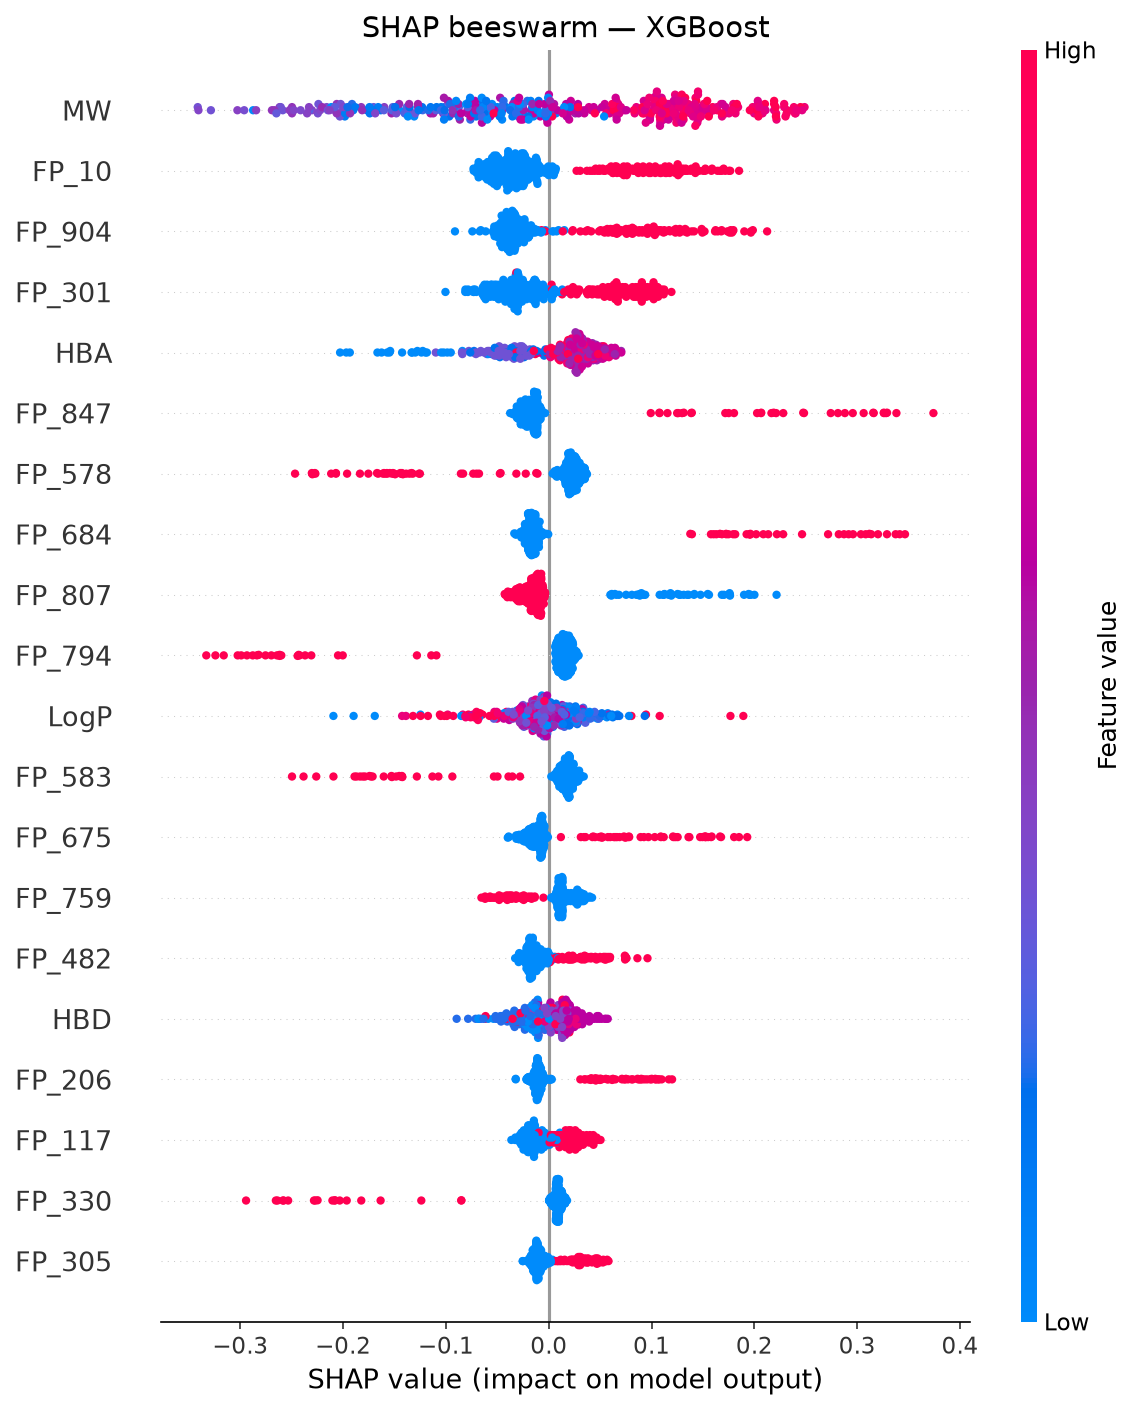
\includegraphics[width=0.80\textwidth]{../figures/fig06_shap_beeswarm.png}
\caption{SHAP Beeswarm Plot แสดงทิศทางอิทธิพลของแต่ละคุณลักษณะ}
\label{fig:beeswarm}
\end{figure}

\begin{figure}[H]
\centering
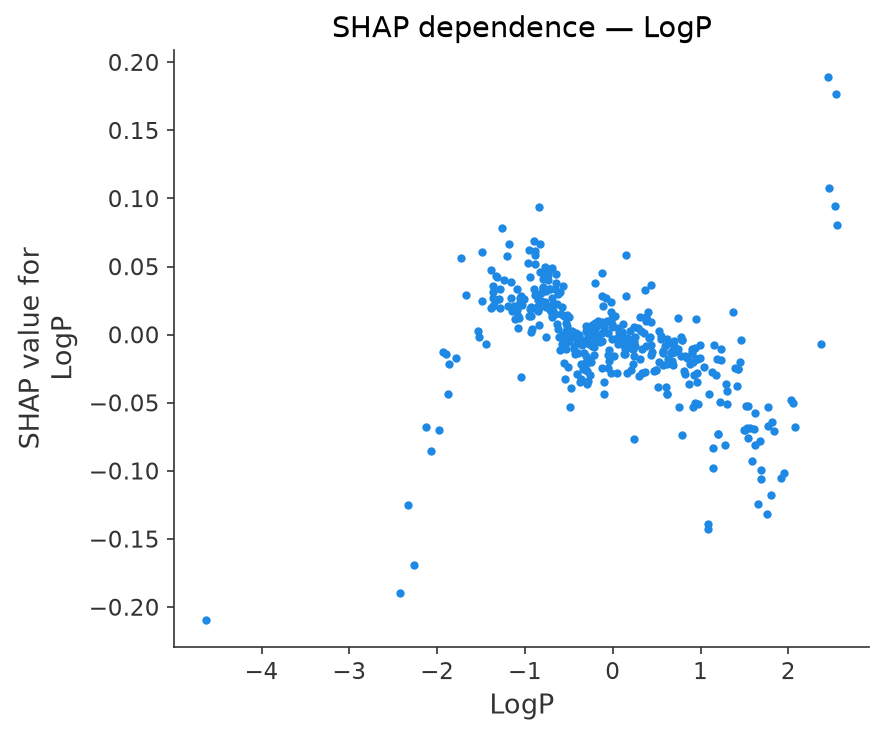
\includegraphics[width=0.72\textwidth]{../figures/fig06b_shap_dependence_logp.png}
\caption{SHAP Dependence Plot ของค่า LogP}
\label{fig:dependence}
\end{figure}

\begin{table}[H]
\centering
\caption{ตารางวิเคราะห์ SAR ของโครงสร้างย่อยที่สำคัญ}
\label{tab:sar}
\small
\begin{tabular}{L{1.8cm} R{1.8cm} L{2.0cm} R{2.0cm} R{1.6cm} R{1.8cm} R{1.6cm}}
\toprule
\textbf{บิต} & \shortstack{\textbf{Mean}\\\textbf{$|$SHAP$|$}} & \textbf{ทิศทาง} & \textbf{SHAP เมื่อบิต=1} & \textbf{\% ใน active} & \textbf{\% ใน inactive} & \textbf{จำนวน โมเลกุล}\\
\midrule
FP\_10 & 0.0561 & เพิ่มฤทธิ์ & $+0.1002$ & \textbf{41.9} & \textbf{4.5} & 696\\
FP\_904 & 0.0557 & เพิ่มฤทธิ์ & $+0.1005$ & 33.6 & 19.7 & 634\\
FP\_301 & 0.0484 & เพิ่มฤทธิ์ & $+0.0710$ & \textbf{50.9} & \textbf{13.1} & 908\\
FP\_578 & 0.0364 & ลดฤทธิ์ & $-0.1417$ & 6.1 & 25.8 & 276\\
FP\_807 & 0.0304 & ลดฤทธิ์ & $-0.0173$ & 84.4 & 95.5 & 1{,}904\\
FP\_794 & 0.0303 & ลดฤทธิ์ & $-0.2509$ & \textbf{2.0} & \textbf{19.7} & 130\\
\bottomrule
\end{tabular}
\end{table}

ผลการวิเคราะห์ SAR ให้ข้อมูลที่ตีความเชิงเคมีได้อย่างสอดคล้องกัน

\textbf{บิตที่เพิ่มฤทธิ์} บิต FP\_301 ปรากฏในสารกลุ่ม active ถึงร้อยละ 50.9 แต่ปรากฏในกลุ่ม inactive เพียงร้อยละ 13.1 คิดเป็นอัตราส่วนความเข้มข้น 3.9 เท่า และบิต FP\_10 มีอัตราส่วนสูงถึง 9.3 เท่า (ร้อยละ 41.9 เทียบกับ 4.5) โมเลกุลตัวอย่างที่มีบิต FP\_10 และมีค่า SHAP สูงสุดคือสารที่มีโครงสร้างเปปไทด์คล้ายพร้อมหมู่แอลดีไฮด์ที่ปลาย ซึ่งเป็นหมู่ที่ทราบกันดีว่าสร้างพันธะโควาเลนต์แบบผันกลับได้กับซิสเตอีนที่ตำแหน่ง 145 ในช่องเร่งปฏิกิริยาของ \Mpro

\textbf{บิตที่ลดฤทธิ์} บิต FP\_794 ปรากฏในกลุ่ม inactive ร้อยละ 19.7 แต่ปรากฏในกลุ่ม active เพียงร้อยละ 2.0 และมีค่า SHAP เฉลี่ยเมื่อบิตถูกเซ็ตติดลบมากที่สุดที่ $-0.2509$ โมเลกุลตัวอย่างเป็นสารกลุ่มพอลิไซคลิกอะโรมาติกที่ไม่มีหมู่ฟังก์ชันสำหรับสร้างพันธะโควาเลนต์

\begin{warnnote}[ข้อสังเกตเชิงระเบียบวิธี]
บิต FP\_807 มีลักษณะพิเศษคือปรากฏในโมเลกุลถึง 1{,}904 ตัวจาก 2{,}198 ตัว (ร้อยละ 86.6) และปรากฏในทั้งกลุ่ม active (ร้อยละ 84.4) และ inactive (ร้อยละ 95.5) ในสัดส่วนใกล้เคียงกัน บิตนี้จึงเป็นโครงสร้างย่อยทั่วไปที่พบได้ในสารเกือบทุกตัว ค่า SHAP ที่ติดลบเล็กน้อยจึงไม่ควรตีความว่าโครงสร้างนี้ลดฤทธิ์อย่างมีความหมายทางเคมี แต่เป็นผลจากการที่แบบจำลองใช้บิตนี้เป็นค่าอ้างอิงพื้นฐานมากกว่า
\end{warnnote}

\begin{figure}[H]
\centering
\begin{tabular}{ccc}
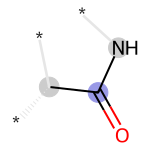
\includegraphics[width=0.24\textwidth]{../figures/fig07_bit_10_substructure.png} &
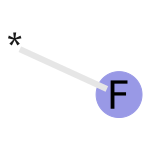
\includegraphics[width=0.24\textwidth]{../figures/fig07_bit_904_substructure.png} &
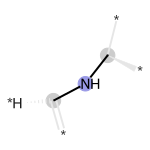
\includegraphics[width=0.24\textwidth]{../figures/fig07_bit_301_substructure.png}\\
(ก) บิต 10 --- เพิ่มฤทธิ์ & (ข) บิต 904 --- เพิ่มฤทธิ์ & (ค) บิต 301 --- เพิ่มฤทธิ์\\[1.2em]
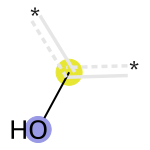
\includegraphics[width=0.24\textwidth]{../figures/fig07_bit_578_substructure.png} &
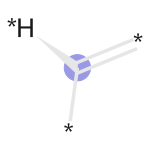
\includegraphics[width=0.24\textwidth]{../figures/fig07_bit_807_substructure.png} &
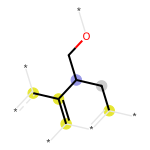
\includegraphics[width=0.24\textwidth]{../figures/fig07_bit_794_substructure.png}\\
(ง) บิต 578 --- ลดฤทธิ์ & (จ) บิต 807 --- ลดฤทธิ์ & (ฉ) บิต 794 --- ลดฤทธิ์\\
\end{tabular}
\caption{โครงสร้างย่อย 2 มิติของบิตสำคัญทั้ง 6 บิตที่ได้จากการจับคู่ย้อนกลับ}
\label{fig:bits}
\end{figure}

\section{ผลการทดสอบข้ามชุดข้อมูล}

\begin{table}[H]
\centering
\caption{ผลการทดสอบข้ามชุดข้อมูลกับ DDH COVID-19}
\label{tab:external}
\begin{tabular}{L{8.4cm} R{4.0cm}}
\toprule
\textbf{ตัวชี้วัด} & \textbf{ค่า}\\
\midrule
จำนวนสาร (หลังตัดที่ซ้ำกับชุดฝึก 4 ตัว) & 90\\
\textbf{\Rsq} & $\mathbf{-1.7191}$\\
RMSE & 1.3504\\
MAE & 1.2031\\
\textbf{Spearman $\rho$} & $\mathbf{0.5203}$\\
ค่าคลาดเคลื่อนเฉลี่ย (Bias) & $\mathbf{+1.1855}$\\
\bottomrule
\end{tabular}
\end{table}

\begin{warnnote}[ผลลบที่ต้องรายงานอย่างตรงไปตรงมา]
ค่า \Rsq\ ที่ติดลบหมายความว่าแบบจำลองทำนายชุด DDH ได้แย่กว่าการทายด้วยค่าเฉลี่ยของชุด DDH เอง และค่า Bias ที่ $+1.1855$ แสดงว่าแบบจำลองทำนายสูงเกินจริงอย่างเป็นระบบถึง 1.19 log unit หรือคิดเป็นการประเมินความแรงเกินจริงประมาณ 15 เท่า
\end{warnnote}

\begin{table}[H]
\centering
\caption{ผลการวิเคราะห์ Applicability Domain}
\label{tab:ad}
\begin{tabular}{L{5.2cm} R{1.7cm} R{2.4cm} R{1.9cm} R{2.1cm}}
\toprule
\textbf{ชุดข้อมูล} & \textbf{จำนวน} & \textbf{Tanimoto เฉลี่ย} & \textbf{มัธยฐาน} & \textbf{\% $< 0.4$}\\
\midrule
ChEMBL test (ในโดเมน) & 550 & 0.7541 & 0.7972 & \textbf{7.6}\\
DDH external & 90 & 0.3340 & 0.2897 & \textbf{84.4}\\
MultiTarget (นอกโดเมน) & 1{,}331 & 0.2880 & 0.2738 & \textbf{95.6}\\
\bottomrule
\end{tabular}
\end{table}

การวิเคราะห์ Applicability Domain อธิบายความล้มเหลวข้างต้นได้อย่างชัดเจน สารในชุด DDH ถึงร้อยละ 84.4 มีค่าความคล้ายคลึง Tanimoto สูงสุดต่อชุดฝึกต่ำกว่าเกณฑ์ 0.4 โดยมีค่ามัธยฐานเพียง 0.2897 ขณะที่ชุดทดสอบภายในมีเพียงร้อยละ 7.6 ที่อยู่นอกเกณฑ์ และมีค่ามัธยฐานสูงถึง 0.7972

กล่าวอีกนัยหนึ่ง ชุด DDH แทบเป็นสารคนละปริภูมิเคมีกับข้อมูลที่ใช้ฝึก โดยมีระดับความแตกต่างใกล้เคียงกับชุด MultiTarget ซึ่งเป็นสารที่ออกฤทธิ์ต่อเป้าหมายคนละชนิดโดยสิ้นเชิง (DRD2, HDAC1, BACE1)

นอกจากนี้ยังมีปัจจัยเสริมคือการเลื่อนของการกระจายตัวแปรตาม (Label Distribution Shift) โดยชุด ChEMBL มี \pICfifty\ เฉลี่ย 6.393 และประกอบด้วยสาร active เป็นส่วนใหญ่ ขณะที่ชุด DDH มีค่าเฉลี่ยเพียง 4.872 และเป็นสาร inactive ถึง 61 จาก 90 ตัว เมื่อประกอบกับจุดอ่อนของแบบจำลองที่ทำนายสาร inactive สูงเกินจริง จึงส่งผลให้ความคลาดเคลื่อนสะสมรุนแรงขึ้น

\begin{keynote}[สิ่งที่ยังใช้ได้]
ค่า Spearman $\rho$ = 0.5203 บ่งชี้ว่าแบบจำลองยังคงจัดอันดับสารได้ในระดับปานกลาง แม้ค่าสัมบูรณ์จะคลาดเคลื่อนมาก ในทางปฏิบัติหมายความว่าแบบจำลองยังพอใช้เป็นเครื่องมือจัดลำดับความสำคัญเพื่อคัดกรองเบื้องต้นได้ แต่ไม่ควรใช้ค่า \pICfifty\ ที่ทำนายได้เป็นตัวเลขสัมบูรณ์กับสารนอกโดเมน
\end{keynote}

\begin{figure}[H]
\centering
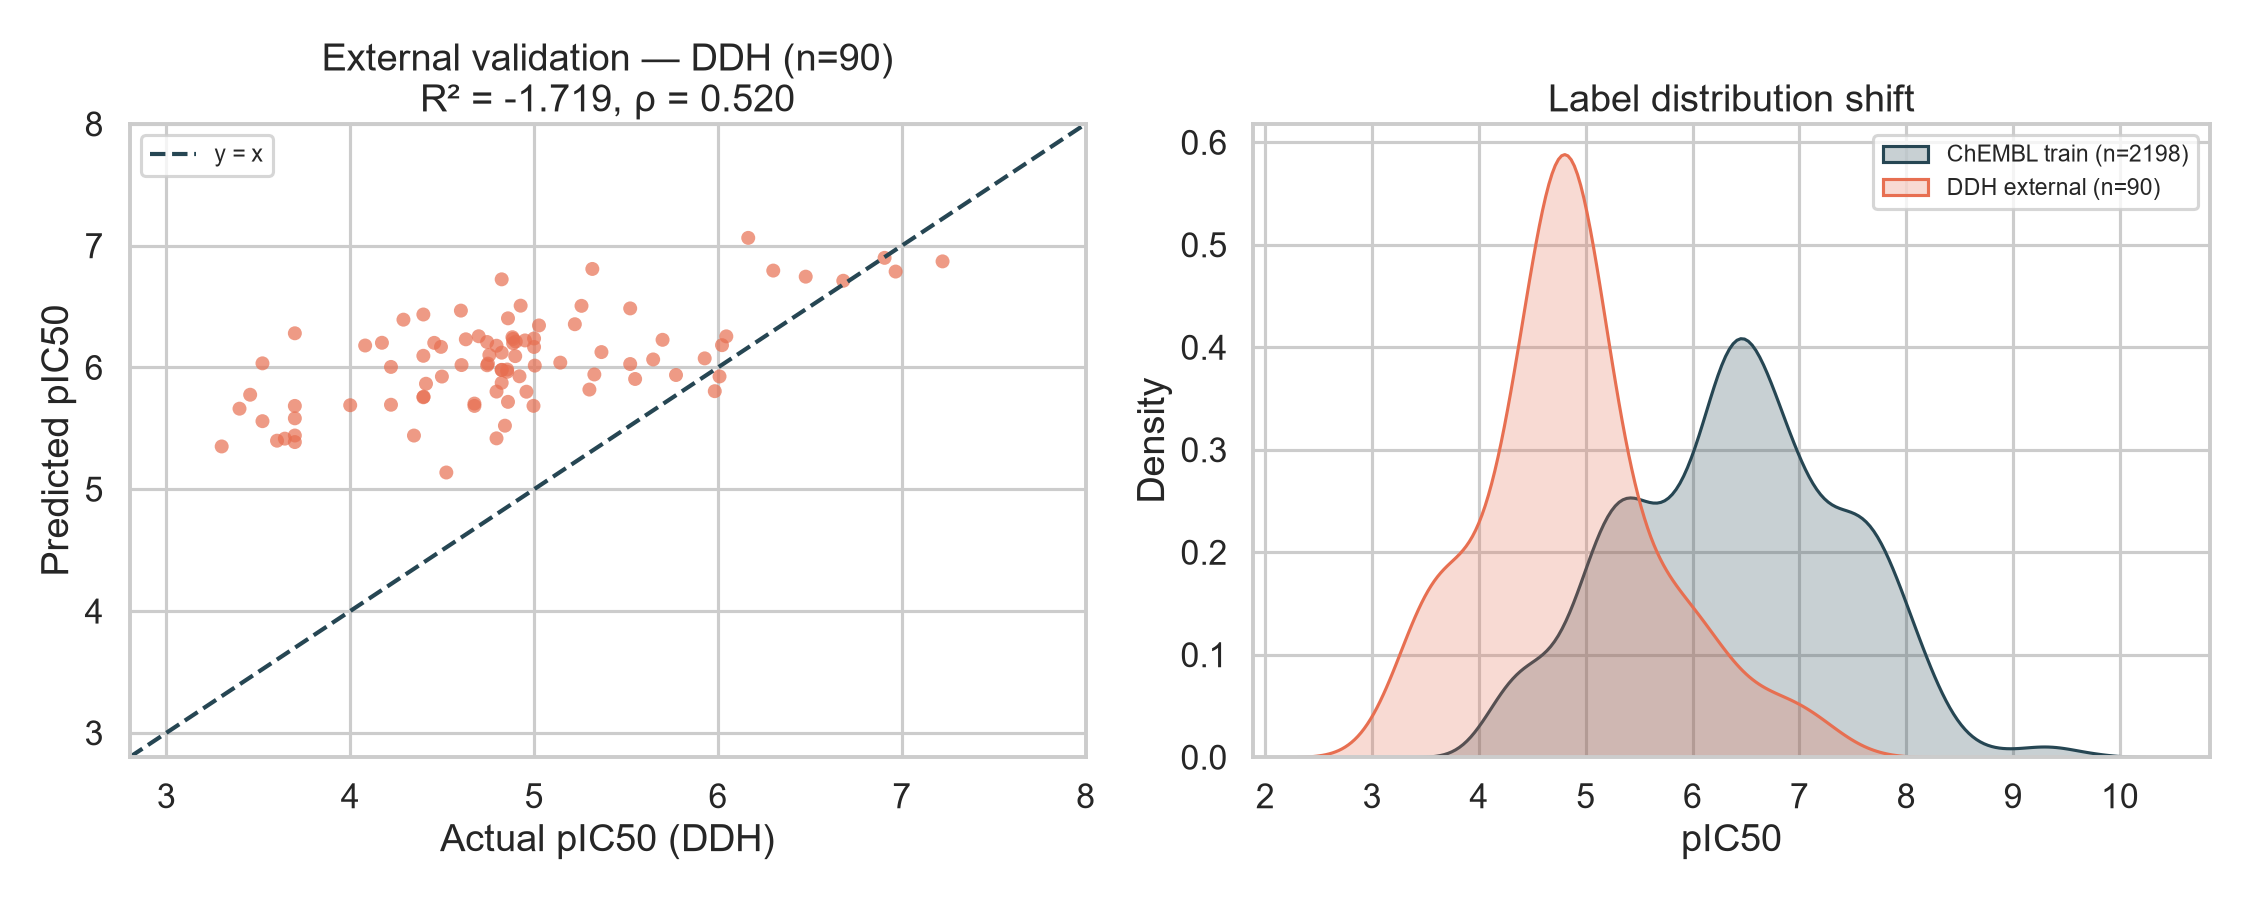
\includegraphics[width=\textwidth]{../figures/fig08_external_validation.png}
\caption{ผลการทดสอบข้ามชุดข้อมูล (ซ้าย) และการเลื่อนของการกระจายตัวแปรตาม (ขวา)}
\label{fig:extval}
\end{figure}

\begin{figure}[H]
\centering
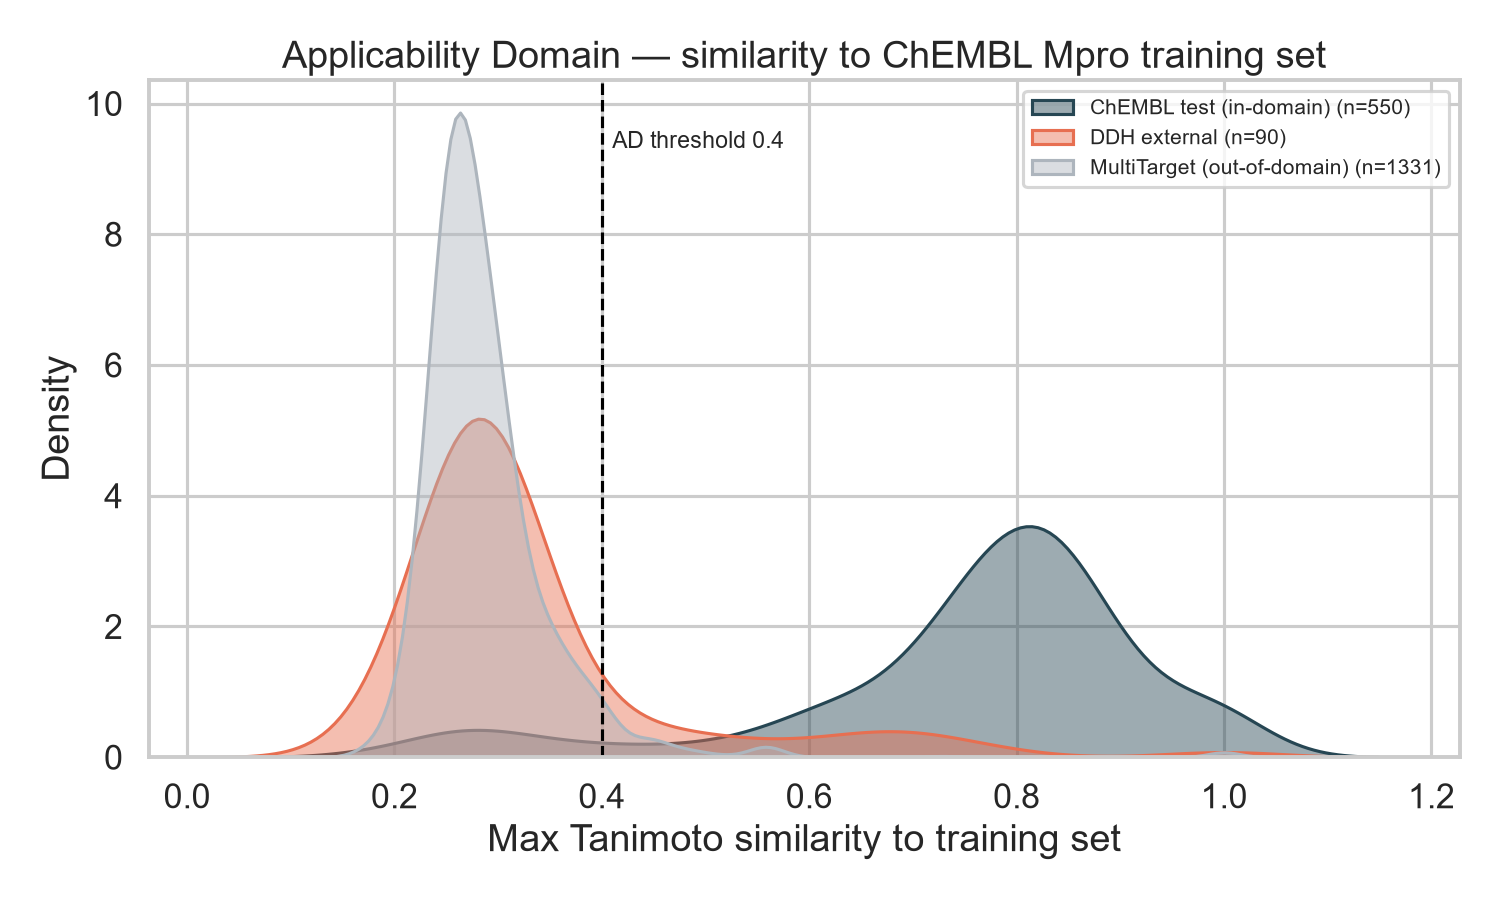
\includegraphics[width=0.82\textwidth]{../figures/fig09_applicability_domain.png}
\caption{การวิเคราะห์ Applicability Domain ด้วยค่าความคล้ายคลึง Tanimoto}
\label{fig:adfig}
\end{figure}

\begin{table}[H]
\centering
\caption{ผลการทำนายสาร BLINDED จำนวน 10 ตัว}
\label{tab:blinded}
\begin{tabular}{C{3.0cm} R{4.0cm} R{4.4cm}}
\toprule
\textbf{ลำดับสาร} & \textbf{\pICfifty\ ที่ทำนาย} & \textbf{\ICfifty\ ที่ทำนาย ($\mu$M)}\\
\midrule
4 & 5.476 & 3.345\\
23 & 5.833 & 1.469\\
28 & 5.810 & 1.549\\
42 & 5.994 & 1.014\\
46 & 6.225 & 0.596\\
58 & 6.546 & 0.285\\
\textbf{63} & \textbf{6.990} & \textbf{0.102}\\
68 & 6.500 & 0.316\\
74 & 6.251 & 0.561\\
95 & 5.868 & 1.355\\
\bottomrule
\end{tabular}
\end{table}

สารลำดับที่ 63 ได้รับการทำนายว่ามีฤทธิ์แรงที่สุด อย่างไรก็ตาม เนื่องจากสารกลุ่มนี้อยู่ในชุด DDH ซึ่งพบว่าอยู่นอก Applicability Domain เป็นส่วนใหญ่ ค่าทำนายเหล่านี้จึงควรถือเป็นเพียงการสาธิตการใช้งานระบบ และควรตีความในเชิงลำดับมากกว่าค่าสัมบูรณ์

\chapter{สรุปผล อภิปรายผล และข้อเสนอแนะ}

\section{สรุปผลการดำเนินงาน}

โครงงานนี้ได้พัฒนาแบบจำลองการเรียนรู้ของเครื่องสำหรับทำนายค่าฤทธิ์การยับยั้งเอนไซม์ SARS-CoV-2 Main Protease ในรูป \pICfifty\ แบบ In Silico โดยดำเนินงานครบทั้ง 9 ระยะตามแผน สรุปผลได้ดังนี้

\textbf{ด้านข้อมูล} รวบรวมข้อมูลจาก ChEMBL เป้าหมาย \texttt{CHEMBL4523582} จำนวน 4{,}867 รายการ กรอง assay เฉพาะที่วัด \CLpro\ เหลือ 2{,}889 รายการ (คัดออกร้อยละ 40.6 ซึ่งเป็น assay ของ nsp3, PLpro และ papain-like protease) ผ่านการทำความสะอาด 13 ขั้นตอน ได้ชุดข้อมูลมาตรฐาน \textbf{2{,}198 โมเลกุลที่ไม่ซ้ำกัน} ประกอบด้วยสาร active 1{,}453 ตัว intermediate 547 ตัว และ inactive 198 ตัว มีความหลากหลายเชิงโครงสร้างสูงโดยมี Murcko Scaffold ไม่ซ้ำ 976 แบบ

\textbf{ด้านแบบจำลอง} XGBoost ให้ประสิทธิภาพสูงสุดบนชุดทดสอบ โดยได้ \Rsq\ = 0.7034, RMSE = 0.5487, MAE = 0.3918 และ Spearman $\rho$ = 0.8415 ซึ่งเหนือกว่าแบบจำลองพื้นฐานอย่างชัดเจน (\Rsq\ = $-0.0000$) การทำนายร้อยละ 93.6 มีความคลาดเคลื่อนไม่เกิน 1 log unit เมื่อประเมินด้วยการแบ่งข้อมูลตามโครงสร้างแกนกลาง ค่า \Rsq\ ลดลงเหลือ 0.5127

\textbf{ด้านการวิเคราะห์ SAR} ระบุคุณลักษณะสำคัญได้ โดยน้ำหนักโมเลกุลมีอิทธิพลสูงสุด (Mean$|$SHAP$|$ = 0.1165) และสามารถจับคู่ย้อนกลับเป็นภาพโครงสร้างย่อย 2 มิติได้ 6 บิต ซึ่งมีการกระจายตัวระหว่างกลุ่ม active และ inactive ที่แตกต่างกันอย่างชัดเจน

\section{อภิปรายผลตามวัตถุประสงค์}

\begin{table}[H]
\centering
\caption{สรุปการบรรลุวัตถุประสงค์}
\label{tab:objectives}
\small
\begin{tabular}{L{5.0cm} C{1.8cm} L{6.6cm}}
\toprule
\textbf{วัตถุประสงค์} & \textbf{สถานะ} & \textbf{หลักฐานสนับสนุน}\\
\midrule
1. พัฒนาและเปรียบเทียบแบบจำลอง ML ทำนาย \pICfifty & บรรลุ & เปรียบเทียบครบ 4 แบบจำลอง บน 2 วิธีการแบ่งข้อมูล ได้ Test \Rsq\ = 0.7034\\
2. สร้างกระบวนการ Hybrid Features ผ่าน Pipeline ที่ปลอด Leakage & บรรลุ & \texttt{src/pipelines.py} ร่วมกับการทดลอง Ablation E3/E4 และการวัดผล Leakage เชิงปริมาณ E5/E5b\\
3. วิเคราะห์ SAR ด้วย SHAP และภาพโครงสร้าง 2 มิติ & บรรลุ & ตาราง Top-20 Mean$|$SHAP$|$, Beeswarm Plot และภาพโครงสร้างย่อย 6 บิต\\
\bottomrule
\end{tabular}
\end{table}

\subsection{อภิปรายวัตถุประสงค์ที่ 1}

แบบจำลองที่พัฒนาขึ้นบรรลุเกณฑ์ ``ดี'' ที่กำหนดไว้ล่วงหน้า (\Rsq\ ในช่วง 0.60--0.75) ค่า RMSE = 0.5487 log unit หมายความว่าโดยเฉลี่ยแบบจำลองทำนายค่า \ICfifty\ คลาดเคลื่อนประมาณ 3.5 เท่า ซึ่งอยู่ในระดับที่ยอมรับได้สำหรับงานคัดกรองเบื้องต้น เนื่องจากความแปรปรวนของการทดลองในห้องปฏิบัติการเองระหว่างห้องปฏิบัติการต่างกันก็อยู่ในระดับใกล้เคียงกัน

ค่า Spearman $\rho$ = 0.8415 ซึ่งสูงกว่าที่ค่า \Rsq\ บ่งชี้ เป็นข้อค้นพบที่มีนัยสำคัญเชิงปฏิบัติ เพราะในงานคัดกรองยาสิ่งที่ต้องการมากที่สุดคือความสามารถ \textbf{จัดลำดับ} สารเพื่อเลือกไปทดสอบจริง ไม่ใช่ความแม่นยำของค่าสัมบูรณ์

ประเด็นที่น่าสังเกตคือ XGBoost ทำได้ต่ำที่สุดในระยะ Cross-Validation ก่อนปรับจูน (CV \Rsq\ = 0.5803) แต่กลับดีที่สุดหลังปรับจูน (Test \Rsq\ = 0.7034) แสดงว่าค่าเริ่มต้นของ XGBoost ไม่เหมาะกับข้อมูลชุดนี้ และการปรับจูนไฮเปอร์พารามิเตอร์มีความสำคัญมากกว่าการเลือกอัลกอริทึม

\subsection{อภิปรายวัตถุประสงค์ที่ 2}

การสร้าง Pipeline ที่ป้องกัน Data Leakage บรรลุผลตามวัตถุประสงค์ในเชิงระเบียบวิธี แต่ \textbf{ผลการวัดเชิงปริมาณไม่เป็นไปตามสมมติฐานตั้งต้น}

สมมติฐานเดิมคาดว่าการปรับสเกลก่อนแบ่งข้อมูลจะทำให้ผลสูงเกินจริงอย่างเห็นได้ชัด แต่ผลการทดลอง E5 พบส่วนต่างเพียง $+0.0001$ \Rsq\ คำอธิบายคือสัดส่วนคุณลักษณะที่ต้องปรับสเกลมีเพียงร้อยละ 0.39 และขนาดชุดข้อมูลใหญ่เพียงพอ

อย่างไรก็ตาม เมื่อออกแบบการทดลองเพิ่มเติม E5b เพื่อตรวจสอบ Feature Selection Leakage ซึ่งเป็นรูปแบบที่ตรวจพบจริงในไฟล์ \texttt{xfinal.csv} ที่ได้รับมอบมา พบอคติบวก $+0.0116$ \Rsq\ ซึ่งมากกว่ารูปแบบแรกถึง 116 เท่า

\begin{keynote}[บทเรียนเชิงระเบียบวิธี]
การใช้ Pipeline ยังคงเป็นแนวปฏิบัติที่ถูกต้องและควรทำเสมอ แต่ผู้วิจัยควรตระหนักว่าความรุนแรงของ Data Leakage ขึ้นอยู่กับ \textbf{สัดส่วนของคุณลักษณะที่ได้รับผลกระทบ} และ \textbf{ขนาดของชุดข้อมูล} การรั่วไหลจากการคัดเลือกคุณลักษณะเป็นภัยคุกคามที่ใหญ่กว่าการรั่วไหลจากการปรับสเกลอย่างมีนัยสำคัญ
\end{keynote}

สำหรับผลการศึกษา Ablation พบว่า Hybrid Features ให้ผลดีที่สุดจริง แต่ส่วนเพิ่มจาก Lipinski Descriptors มีเพียง $+0.0112$ \Rsq\ ขณะที่การวิเคราะห์ SHAP กลับพบว่า Lipinski ติดอันดับ 20 แรกครบทั้ง 4 ตัว และ MW เป็นอันดับ 1 ผลสองอย่างนี้ไม่ขัดแย้งกัน แต่สะท้อนปรากฏการณ์ \textbf{คุณลักษณะสำคัญแต่ซ้ำซ้อน} เพราะ Morgan Fingerprints เข้ารหัสข้อมูลขนาดโมเลกุลไว้โดยอ้อมอยู่แล้ว

\subsection{อภิปรายวัตถุประสงค์ที่ 3}

การวิเคราะห์ SAR ให้ผลที่ตีความเชิงเคมีได้อย่างสอดคล้อง โดยเฉพาะบิต FP\_10 ที่มีอัตราส่วนความเข้มข้นระหว่างกลุ่ม active ต่อ inactive สูงถึง 9.3 เท่า และโมเลกุลตัวอย่างมีหมู่แอลดีไฮด์ซึ่งเป็นหมู่ที่ทราบกันว่าสร้างพันธะกับซิสเตอีนในช่องเร่งปฏิกิริยาของ \Mpro\ ได้

อย่างไรก็ตาม ต้องย้ำข้อจำกัดที่ประกาศไว้ตั้งแต่ต้นว่า ผลการวิเคราะห์ SHAP แสดง \textbf{ความสัมพันธ์เชิงสถิติ} ระหว่างชิ้นส่วนโมเลกุลกับค่าที่แบบจำลองทำนาย ไม่สามารถอ้างเป็น \textbf{กลไกการจับทางชีวภาพเชิงสาเหตุ} ในระดับ 3 มิติได้ ความสอดคล้องกับความรู้ทางเคมียาที่พบเป็นเพียงหลักฐานสนับสนุนความสมเหตุสมผล ไม่ใช่การพิสูจน์กลไก การยืนยันที่แท้จริงต้องอาศัย Molecular Docking, Molecular Dynamics และการทดสอบ In Vitro

กรณีบิต FP\_807 เป็นตัวอย่างที่ดีของความจำเป็นในการตรวจสอบผล SHAP ด้วยสถิติเชิงพรรณนาประกอบ เนื่องจากบิตนี้ปรากฏในโมเลกุลถึงร้อยละ 86.6 ทั้งในกลุ่ม active และ inactive ค่า SHAP ที่ติดลบจึงไม่มีความหมายเชิงเคมีที่ตีความได้ หากรายงานเฉพาะอันดับ Mean$|$SHAP$|$ โดยไม่ดูสัดส่วนการปรากฏ อาจนำไปสู่การตีความที่ผิดพลาด

\section{ข้อค้นพบสำคัญที่นอกเหนือจากวัตถุประสงค์}

\subsection{ความล้มเหลวของการทดสอบข้ามชุดข้อมูล}

ข้อค้นพบที่มีคุณค่าที่สุดของโครงงานนี้อาจเป็นผลลบ กล่าวคือ แบบจำลองที่ได้ค่า \Rsq\ = 0.7034 บนชุดทดสอบภายใน กลับได้ \Rsq\ = $-1.72$ เมื่อทดสอบกับสาร COVID-19 จากแหล่งอิสระ 90 ตัว

การวิเคราะห์ Applicability Domain อธิบายสาเหตุได้อย่างชัดเจนว่า ร้อยละ 84.4 ของสารในชุดทดสอบข้ามแหล่งมีค่าความคล้ายคลึง Tanimoto ต่อชุดฝึกต่ำกว่า 0.4 ซึ่งใกล้เคียงกับชุดสารที่ออกฤทธิ์ต่อเป้าหมายคนละชนิดโดยสิ้นเชิง

\begin{keynote}[นัยเชิงวิชาการ]
ผลนี้เป็นหลักฐานเชิงประจักษ์ที่สนับสนุนข้อวิจารณ์ที่มีต่องานวิจัย QSAR จำนวนมากที่รายงานเฉพาะค่า \Rsq\ บนชุดทดสอบภายใน โดยไม่ประเมิน Applicability Domain หรือทดสอบข้ามแหล่งข้อมูล ค่า \Rsq\ ที่สูงในการแบ่งข้อมูลแบบสุ่มไม่ได้รับประกันความสามารถทำนายในทางปฏิบัติเลย
\end{keynote}

\subsection{ผลกระทบของความไม่สมดุลของข้อมูล}

การวิเคราะห์ค่าคลาดเคลื่อนแยกตามกลุ่มฤทธิ์เผยให้เห็นว่า แบบจำลองทำนายสาร inactive สูงเกินจริงอย่างเป็นระบบเฉลี่ย 0.72 log unit ซึ่งเป็นผลจากอัตราส่วนสาร active ต่อ inactive ในชุดฝึกที่ 7.3 ต่อ 1

ข้อค้นพบนี้เชื่อมโยงโดยตรงกับความล้มเหลวในหัวข้อก่อนหน้า เพราะชุด DDH ประกอบด้วยสาร inactive ถึง 61 จาก 90 ตัว จึงตกอยู่ในสถานการณ์ที่แบบจำลองอ่อนแอที่สุดพอดี ความไม่สมดุลของข้อมูลจึงไม่ได้ส่งผลเฉพาะในงานจำแนกประเภทเท่านั้น แต่ส่งผลต่องานถดถอยด้วยเมื่อการกระจายของตัวแปรตามไม่สมมาตร

\subsection{ข้อจำกัดของ Morgan Fingerprints กับสเตอริโอเคมี}

การวิเคราะห์ Activity Cliff พบคู่โมเลกุลที่มีความคล้ายคลึงเกิน 0.85 จำนวน 635 คู่ ในจำนวนนี้มี 23 คู่ (ร้อยละ 3.62) ที่มีค่า \pICfifty\ ต่างกันเกิน 1.5 log unit

เมื่อตรวจสอบคู่ที่รุนแรงที่สุดพบว่าเป็น \textbf{สเตอริโอไอโซเมอร์} ตัวอย่างเช่น สาร CHEMBL5412571 มี \pICfifty\ = 8.52 ขณะที่ CHEMBL5197241 มี \pICfifty\ = 6.33 ทั้งสองมีสูตรโครงสร้างเชิงเส้นเหมือนกันทุกประการ ต่างกันเพียงการจัดเรียงสเตอริโอที่ศูนย์กลางไครัลสองตำแหน่ง แต่มีฤทธิ์ต่างกันถึง 2.19 log unit หรือประมาณ 155 เท่า

ค่าความคล้ายคลึง Tanimoto ระหว่างสองโมเลกุลนี้เท่ากับ \textbf{1.000 พอดี} เนื่องจาก Morgan Fingerprints ที่ตั้งค่าตามปกติไม่บันทึกข้อมูลสเตอริโอเคมี แบบจำลองจึงได้รับเวกเตอร์คุณลักษณะที่เหมือนกันทุกประการสำหรับโมเลกุลสองตัวที่มีฤทธิ์ต่างกันมหาศาล และไม่มีทางทำนายทั้งคู่ให้ถูกต้องพร้อมกันได้

ข้อค้นพบนี้มีความสำคัญมากในบริบทของสารยับยั้ง \Mpro\ เพราะสารกลุ่มนี้จำนวนมากมีลักษณะคล้ายเปปไทด์ซึ่งมีศูนย์กลางไครัลหลายตำแหน่ง และการจับกับโปรตีนขึ้นอยู่กับรูปทรงสามมิติอย่างมาก

\section{ข้อจำกัดของการศึกษา}

\begin{enumerate}[leftmargin=2em, itemsep=0.4em]
  \item \textbf{เป็นการศึกษา In Silico เท่านั้น} ไม่มีการยืนยันผลในห้องปฏิบัติการ สารที่แบบจำลองทำนายว่ามีฤทธิ์แรงยังไม่ได้รับการทดสอบจริง
  \item \textbf{SHAP แสดงความสัมพันธ์เชิงสถิติ ไม่ใช่กลไกเชิงสาเหตุ} โครงสร้างย่อยที่ระบุได้เป็นเพียงรูปแบบทางสถิติที่แบบจำลองเรียนรู้ ไม่ใช่การพิสูจน์ว่าโครงสร้างนั้นทำหน้าที่จับกับเอนไซม์จริง
  \item \textbf{ข้อมูลมาจากหลายห้องปฏิบัติการและหลายโปรโตคอล} แม้จะกรอง assay เฉพาะ \CLpro\ แล้ว แต่วิธีการวัด ความเข้มข้นของเอนไซม์ และชนิดสับสเตรตที่ต่างกันยังเป็นแหล่งความแปรปรวนในตัวแปรตาม
  \item \textbf{คุณลักษณะไม่ครอบคลุมสเตอริโอเคมี} ซึ่งเป็นข้อจำกัดเชิงหลักการที่ส่งผลต่อความสามารถทำนายสารกลุ่มเปปไทด์คล้าย
  \item \textbf{ความสามารถทำนายจำกัดอยู่ในปริภูมิเคมีของชุดฝึก} ตามที่พิสูจน์แล้วด้วยการทดสอบข้ามชุดข้อมูล
  \item \textbf{ไม่ครอบคลุม Molecular Docking และ Molecular Dynamics} ตามขอบเขตที่ประกาศไว้
\end{enumerate}

\section{ข้อเสนอแนะ}

\subsection{ข้อเสนอแนะสำหรับการนำผลไปใช้}

\begin{enumerate}[leftmargin=2em, itemsep=0.4em]
  \item \textbf{ใช้แบบจำลองเป็นเครื่องมือจัดลำดับความสำคัญ ไม่ใช่เครื่องมือวัดค่าสัมบูรณ์} เนื่องจากค่า Spearman $\rho$ สูงกว่าที่ค่า \Rsq\ บ่งชี้ การใช้แบบจำลองเพื่อเรียงลำดับสารก่อนนำไปทดสอบจริงจะให้ประโยชน์สูงสุด
  \item \textbf{ตรวจสอบ Applicability Domain ก่อนใช้ทุกครั้ง} ควรคำนวณค่า Tanimoto สูงสุดต่อชุดฝึกก่อนเชื่อผลทำนาย หากต่ำกว่า 0.4 ควรถือว่าผลทำนายไม่น่าเชื่อถือ
  \item \textbf{อ้างอิงค่า \Rsq\ = 0.5127 จาก Scaffold Split} เมื่อสื่อสารความสามารถของแบบจำลองในการทำนายสารที่มีโครงสร้างแกนกลางใหม่
\end{enumerate}

\subsection{ข้อเสนอแนะสำหรับการพัฒนาต่อยอด}

\begin{enumerate}[leftmargin=2em, itemsep=0.4em]
  \item \textbf{เปิดใช้งานสเตอริโอเคมีในการสกัด Fingerprints} โดยตั้งค่า \texttt{includeChirality=True} ซึ่งจะช่วยแก้ปัญหาสเตอริโอไอโซเมอร์ได้โดยตรง คาดว่าจะเป็นการปรับปรุงที่ให้ผลตอบแทนสูงที่สุดเมื่อเทียบกับความพยายามที่ใช้
  \item \textbf{แก้ปัญหาความไม่สมดุลของข้อมูล} ด้วยการเพิ่มน้ำหนักตัวอย่างสาร inactive ในฟังก์ชันสูญเสีย หรือรวบรวมข้อมูลสาร inactive เพิ่มเติมจากฐานข้อมูล PubChem BioAssay
  \item \textbf{ทดลองใช้คุณลักษณะเพิ่มเติม} เช่น RDKit Descriptors ชุดเต็ม, MACCS Keys หรือ Pharmacophore Fingerprints เพื่อเพิ่มมิติของสารสนเทศ
  \item \textbf{ทดลองใช้แบบจำลองที่เรียนรู้การแทนโครงสร้างเอง} เช่น Graph Neural Networks (GNN) ซึ่งรับโครงสร้างโมเลกุลเป็นกราฟโดยตรง และสามารถเข้ารหัสสเตอริโอเคมีได้
  \item \textbf{สร้างแบบจำลองประมาณความไม่แน่นอน} เช่น Conformal Prediction หรือ Ensemble Variance เพื่อให้แบบจำลองสามารถบอกได้ว่าตัวเองไม่มั่นใจเมื่อใด ซึ่งจะช่วยลดปัญหาการทำนายสารนอกโดเมน
  \item \textbf{พัฒนาเว็บแอปพลิเคชันคัดกรองตัวยา} โดยรับ SMILES เป็นข้อมูลนำเข้า แล้วแสดงค่า \pICfifty\ ที่ทำนาย พร้อมค่าความคล้ายคลึงต่อชุดฝึกเป็นตัวบ่งชี้ความน่าเชื่อถือ และภาพโครงสร้างย่อยที่มีอิทธิพลต่อการทำนาย
\end{enumerate}

\subsection{ข้อเสนอแนะเชิงระเบียบวิธีสำหรับงาน QSAR}

\begin{enumerate}[leftmargin=2em, itemsep=0.4em]
  \item \textbf{รายงานผลทั้ง Random Split และ Scaffold Split ควบคู่กันเสมอ} เพื่อให้ผู้อ่านเห็นภาพความสามารถทำนายที่แท้จริง
  \item \textbf{ประเมินและรายงาน Applicability Domain เป็นส่วนหนึ่งของผลลัพธ์มาตรฐาน} ไม่ใช่การวิเคราะห์เสริม
  \item \textbf{ตรวจสอบการซ้อนทับระหว่างชุดฝึกกับชุดทดสอบข้ามแหล่งด้วย InChIKey เสมอ} ในโครงงานนี้พบสารซ้ำ 4 ตัวซึ่งหากไม่ตัดออกจะทำให้ผลการทดสอบข้ามชุดข้อมูลไม่ถูกต้อง
  \item \textbf{วิเคราะห์ค่าคลาดเคลื่อนแยกตามกลุ่มย่อย} ไม่ใช่รายงานเฉพาะค่ารวม เพราะค่ารวมอาจซ่อนจุดอ่อนเชิงระบบไว้ ดังกรณีสาร inactive ในโครงงานนี้
  \item \textbf{ตรวจสอบผล SHAP ด้วยสถิติเชิงพรรณนาประกอบ} เช่น สัดส่วนการปรากฏของบิตในแต่ละกลุ่ม เพื่อป้องกันการตีความผิดพลาดดังกรณีบิต FP\_807
\end{enumerate}


% ---------- ส่วนท้าย (Back Matter) ----------
% ---------------- เอกสารอ้างอิง ----------------
\chapter*{เอกสารอ้างอิง}
\addcontentsline{toc}{chapter}{เอกสารอ้างอิง}
\markboth{เอกสารอ้างอิง}{เอกสารอ้างอิง}

\begin{enumerate}[leftmargin=2.2em, itemsep=0.75em, label={[\arabic*]}]

\item Jin, Z., Du, X., Xu, Y., Deng, Y., Liu, M., Zhao, Y., \ldots\ \& Yang, H. (2020). Structure of \Mpro\ from SARS-CoV-2 and discovery of its inhibitors. \textit{Nature}, 582(7811), 289--293. \url{https://doi.org/10.1038/s41586-020-2223-y}

\item Gaulton, A., Hersey, A., Nowotka, M., Bento, A. P., Chambers, J., Mendez, D., \ldots\ \& Overington, J. P. (2017). The ChEMBL database in 2017. \textit{Nucleic Acids Research}, 45(D1), D945--D954. \url{https://doi.org/10.1093/nar/gkw1074}

\item Rogers, D., \& Hahn, M. (2010). Extended-connectivity fingerprints. \textit{Journal of Chemical Information and Modeling}, 50(5), 742--754. \url{https://doi.org/10.1021/ci100050t}

\item Lipinski, C. A., Lombardo, F., Dominy, B. W., \& Feeney, P. J. (2001). Experimental and computational approaches to estimate solubility and permeability in drug discovery and development settings. \textit{Advanced Drug Delivery Reviews}, 46(1-3), 3--26. \url{https://doi.org/10.1016/S0169-409X(00)00129-0}

\item Nantasenamat, C., Isarankura-Na-Ayudhya, C., Naenna, T., \& Prachayasittikul, V. (2010). A practical overview of quantitative structure-activity relationship. \textit{EXCLI Journal}, 9, 74--93. \url{https://www.ncbi.nlm.nih.gov/pmc/articles/PMC5084994/}

\item Breiman, L. (2001). Random Forests. \textit{Machine Learning}, 45(1), 5--32. \url{https://doi.org/10.1023/A:1010933404324}

\item Chen, T., \& Guestrin, C. (2016). XGBoost: A scalable tree boosting system. In \textit{Proceedings of the 22nd ACM SIGKDD International Conference on Knowledge Discovery and Data Mining} (pp. 785--794). \url{https://doi.org/10.1145/2939672.2939785}

\item Rodríguez-Pérez, R., \& Bajorath, J. (2020). Interpretation of machine learning predictions using Shapley values: Application to compound activity and property prediction. \textit{Molecular Informatics}, 39(1-2), 1900131. \url{https://doi.org/10.1002/minf.201900131}

\item Bemis, G. W., \& Murcko, M. A. (1996). The properties of known drugs. 1. Molecular frameworks. \textit{Journal of Medicinal Chemistry}, 39(15), 2887--2893. \url{https://doi.org/10.1021/jm9602928}

\item Sheridan, R. P. (2013). Time-split cross-validation as a method for estimating the goodness of prospective prediction. \textit{Journal of Chemical Information and Modeling}, 53(4), 783--790. \url{https://doi.org/10.1021/ci400084k}

\item Lundberg, S. M., \& Lee, S. I. (2017). A unified approach to interpreting model predictions. In \textit{Advances in Neural Information Processing Systems 30} (pp. 4765--4774).

\item Maggiora, G. M. (2006). On outliers and activity cliffs --- Why QSAR often disappoints. \textit{Journal of Chemical Information and Modeling}, 46(4), 1535. \url{https://doi.org/10.1021/ci060117s}

\item Pedregosa, F., Varoquaux, G., Gramfort, A., Michel, V., Thirion, B., Grisel, O., \ldots\ \& Duchesnay, É. (2011). Scikit-learn: Machine learning in Python. \textit{Journal of Machine Learning Research}, 12, 2825--2830.

\item Landrum, G. (2024). \textit{RDKit: Open-source cheminformatics}. \url{https://www.rdkit.org}

\end{enumerate}


% ---------- ภาคผนวก (Appendices) ----------
\appendix
% ==========================================================
%  appendix_a_code.tex — ภาคผนวก ก: โครงสร้างไฟล์และโค้ดโปรแกรม
% ==========================================================

\chapter{โครงสร้างไฟล์และโค้ดโปรแกรม}

\section{โครงสร้างโปรเจกต์}

\begingroup\scriptsize
\begin{verbatim}
SilicoBioactivityPredict/
├── .venv/                          project virtual environment
├── Data_set/                       original raw data (read-only)
├── Docs/
│   ├── Machine Learning ....pdf    project proposal
│   └── Project_Plan.md             execution plan
├── data/
│   ├── raw/                        raw ChEMBL API output
│   ├── interim/                    after assay filtering
│   └── processed/
│       ├── clean_bioactivity_master.csv    2,198 molecules
│       ├── features_hybrid.parquet         1,028 features
│       ├── bitinfo.pkl                     Morgan bit info
│       ├── predictions_test.csv
│       └── predictions_external_ddh.csv
├── src/                            source code, 11 files
│   ├── config.py                   global constants
│   ├── acquire.py                  Phase 1
│   ├── clean.py                    Phase 2
│   ├── features.py                 Phase 3
│   ├── eda.py                      Phase 4
│   ├── pipelines.py                Pipeline + Scaffold Split
│   ├── model_cv.py                 Phase 5
│   ├── tune_eval.py                Phase 6
│   ├── explain.py                  Phase 7
│   ├── external_validation.py      Phase 8
│   └── make_report.py              automated report builder
├── models/best_model_xgboost_20260908.joblib
├── reports/
│   ├── figures/                    18 figures
│   ├── tables/                     10 result tables
│   ├── latex/                      LaTeX source of this report
│   └── final_report.md
├── requirements.txt
└── README.md
\end{verbatim}
\endgroup

\section{ลำดับการรันโปรแกรม}

\begingroup\scriptsize
\begin{verbatim}
cd src && ../.venv/Scripts/python.exe acquire.py
cd src && ../.venv/Scripts/python.exe clean.py
cd src && ../.venv/Scripts/python.exe features.py
cd src && ../.venv/Scripts/python.exe eda.py
cd src && ../.venv/Scripts/python.exe model_cv.py
cd src && ../.venv/Scripts/python.exe tune_eval.py
cd src && ../.venv/Scripts/python.exe explain.py
cd src && ../.venv/Scripts/python.exe external_validation.py
cd src && ../.venv/Scripts/python.exe make_report.py
\end{verbatim}
\endgroup

\section{โค้ดสำคัญ: Pipeline ป้องกัน Data Leakage}

\begingroup\scriptsize
\begin{verbatim}
from sklearn.pipeline import Pipeline
from sklearn.compose import ColumnTransformer
from sklearn.preprocessing import StandardScaler

def make_pipe(estimator, fp_cols=FP_COLS, desc_cols=DESC_COLS):
    transformers = []
    if fp_cols:
        transformers.append(("fp", "passthrough", list(fp_cols)))
    if desc_cols:
        transformers.append(("desc", StandardScaler(), list(desc_cols)))
    prep = ColumnTransformer(transformers, remainder="drop")
    return Pipeline([("prep", prep), ("model", estimator)])
\end{verbatim}
\endgroup

\section{โค้ดสำคัญ: Scaffold Split}

\begingroup\scriptsize
\begin{verbatim}
from collections import defaultdict
from rdkit.Chem.Scaffolds import MurckoScaffold

def scaffold_split(smiles_list, test_frac=0.25):
    buckets = defaultdict(list)
    for i, s in enumerate(smiles_list):
        sc = MurckoScaffold.MurckoScaffoldSmiles(
            smiles=s, includeChirality=False)
        buckets[sc].append(i)
    groups = sorted(buckets.values(), key=len, reverse=True)
    n_train = len(smiles_list) - int(len(smiles_list) * test_frac)
    train, test = [], []
    for g in groups:
        (train if len(train) + len(g) <= n_train else test).extend(g)
    return np.array(train), np.array(test)
\end{verbatim}
\endgroup

\section{โค้ดสำคัญ: การสกัดคุณลักษณะแบบผสม}

\begin{verbatim}
from rdkit import Chem
from rdkit.Chem import Descriptors, Lipinski, rdFingerprintGenerator

gen = rdFingerprintGenerator.GetMorganGenerator(radius=2, fpSize=1024)

def featurize(smiles):
    mol = Chem.MolFromSmiles(smiles)
    ao = rdFingerprintGenerator.AdditionalOutput()
    ao.AllocateBitInfoMap()
    fp = gen.GetFingerprintAsNumPy(mol, additionalOutput=ao)
    desc = [Descriptors.MolWt(mol), Descriptors.MolLogP(mol),
            Lipinski.NumHDonors(mol), Lipinski.NumHAcceptors(mol)]
    return fp, desc, ao.GetBitInfoMap()
\end{verbatim}

% ==========================================================
%  appendix_b_files.tex — ภาคผนวก ข: รายการไฟล์ผลลัพธ์
% ==========================================================

\chapter{รายการไฟล์ผลลัพธ์}

\section{รายการภาพประกอบ}

\begin{table}[H]
\centering
\small
\caption{รายการภาพประกอบผลการดำเนินงาน}\label{tab:figlist}
\begin{tabular}{L{6.6cm} L{7.4cm}}
\toprule
\textbf{ไฟล์} & \textbf{เนื้อหา}\\
\midrule
\texttt{fig01\_pic50\_distribution.png} & การแจกแจงความถี่ของค่า \pICfifty\\
\texttt{fig02\_chemical\_space\_mw\_logp.png} & ปริภูมิเคมี MW เทียบ LogP แยกตามกลุ่มฤทธิ์\\
\texttt{fig02b\_lipinski\_by\_class.png} & Box plot ของ Lipinski Descriptors ตามกลุ่มฤทธิ์\\
\texttt{fig02c\_chemspace\_3sets.png} & เปรียบเทียบปริภูมิเคมีของชุดข้อมูลสามชุด\\
\texttt{fig03\_model\_comparison.png} & เปรียบเทียบประสิทธิภาพ CV เทียบชุดทดสอบ\\
\texttt{fig04\_residual\_plot.png} & กราฟค่าทำนายเทียบค่าจริงและกราฟค่าคลาดเคลื่อน\\
\texttt{fig04b\_residual\_hist.png} & การแจกแจงค่าคลาดเคลื่อน\\
\texttt{fig05\_shap\_bar\_top20.png} & ค่าความสำคัญของคุณลักษณะ 20 อันดับแรก\\
\texttt{fig06\_shap\_beeswarm.png} & SHAP Beeswarm Plot\\
\texttt{fig06b\_shap\_dependence\_logp.png} & SHAP Dependence Plot ของ LogP\\
\texttt{fig07\_bit\_10\_substructure.png} & โครงสร้างย่อยของบิต 10 (เพิ่มฤทธิ์)\\
\texttt{fig07\_bit\_904\_substructure.png} & โครงสร้างย่อยของบิต 904 (เพิ่มฤทธิ์)\\
\texttt{fig07\_bit\_301\_substructure.png} & โครงสร้างย่อยของบิต 301 (เพิ่มฤทธิ์)\\
\texttt{fig07\_bit\_578\_substructure.png} & โครงสร้างย่อยของบิต 578 (ลดฤทธิ์)\\
\texttt{fig07\_bit\_807\_substructure.png} & โครงสร้างย่อยของบิต 807 (ลดฤทธิ์)\\
\texttt{fig07\_bit\_794\_substructure.png} & โครงสร้างย่อยของบิต 794 (ลดฤทธิ์)\\
\texttt{fig08\_external\_validation.png} & ผลการทดสอบข้ามชุดข้อมูล\\
\texttt{fig09\_applicability\_domain.png} & การวิเคราะห์ Applicability Domain\\
\bottomrule
\end{tabular}
\end{table}

\section{รายการตารางผลลัพธ์ดิบ}

\begin{table}[H]
\centering
\caption{รายการไฟล์ตารางผลลัพธ์}
\label{tab:tablist}
\begin{tabular}{L{6.4cm} L{7.4cm}}
\toprule
\textbf{ไฟล์} & \textbf{เนื้อหา}\\
\midrule
\texttt{tbl01\_dataset\_summary.csv} & สรุปคุณลักษณะชุดข้อมูล\\
\texttt{tbl01b\_lipinski\_mannwhitney.csv} & ผลทดสอบ Mann-Whitney U\\
\texttt{tbl01c\_top\_scaffolds.csv} & Murcko Scaffold 10 อันดับแรก\\
\texttt{tbl02\_cv\_results.csv} & ผล Cross-Validation ทุกการทดลอง\\
\texttt{tbl03\_test\_results.csv} & ผลการประเมินบนชุดทดสอบ\\
\texttt{tbl04\_shap\_importance\_top50.csv} & ค่าความสำคัญคุณลักษณะ 50 อันดับแรก\\
\texttt{tbl05\_sar\_bits.csv} & ตารางวิเคราะห์ SAR\\
\texttt{tbl06\_applicability\_domain.csv} & ผลวิเคราะห์ Applicability Domain\\
\texttt{tbl07\_blinded\_predictions.csv} & ผลทำนายสาร BLINDED\\
\texttt{tbl08\_external\_metrics.csv} & ตัวชี้วัดการทดสอบข้ามชุดข้อมูล\\
\bottomrule
\end{tabular}
\end{table}


\end{document}
